\documentclass{book}
\usepackage[a4paper,top=2.5cm,bottom=2.5cm,left=2.5cm,right=2.5cm]{geometry}
\usepackage{makeidx}
\usepackage{natbib}
\usepackage{graphicx}
\usepackage{multicol}
\usepackage{float}
\usepackage{listings}
\usepackage{color}
\usepackage{ifthen}
\usepackage[table]{xcolor}
\usepackage{textcomp}
\usepackage{alltt}
\usepackage{ifpdf}
\ifpdf
\usepackage[pdftex,
            pagebackref=true,
            colorlinks=true,
            linkcolor=blue,
            unicode
           ]{hyperref}
\else
\usepackage[ps2pdf,
            pagebackref=true,
            colorlinks=true,
            linkcolor=blue,
            unicode
           ]{hyperref}
\usepackage{pspicture}
\fi
\usepackage[utf8]{inputenc}
\usepackage{mathptmx}
\usepackage[scaled=.90]{helvet}
\usepackage{courier}
\usepackage{sectsty}
\usepackage{amssymb}
\usepackage[titles]{tocloft}
\usepackage{doxygen}
\lstset{language=C++,inputencoding=utf8,basicstyle=\footnotesize,breaklines=true,breakatwhitespace=true,tabsize=4,numbers=left }
\makeindex
\setcounter{tocdepth}{3}
\renewcommand{\footrulewidth}{0.4pt}
\renewcommand{\familydefault}{\sfdefault}
\hfuzz=15pt
\setlength{\emergencystretch}{15pt}
\hbadness=750
\tolerance=750
\begin{document}
\hypersetup{pageanchor=false,citecolor=blue}
\begin{titlepage}
\vspace*{7cm}
\begin{center}
{\Large Sleepy Mustache }\\
\vspace*{1cm}
{\large Generated by Doxygen 1.8.2}\\
\vspace*{0.5cm}
{\small Fri Jul 12 2013 12:36:14}\\
\end{center}
\end{titlepage}
\clearemptydoublepage
\pagenumbering{roman}
\tableofcontents
\clearemptydoublepage
\pagenumbering{arabic}
\hypersetup{pageanchor=true,citecolor=blue}
\chapter{$<$$|$\-:\{)}
\label{index}\hypertarget{index}{}\section*{sleepy-\/mustache}

Doxygen \href{documentation/html/index.html}{\tt Documentation} is available.

Sleepy mustache is a P\-H\-P framework that comes with solutions for everyday php challenges. All the functionality is optional and tries to be as minimalist as possible.

\subsection*{Included Functionality}


\begin{DoxyItemize}
\item Hooks
\item Templating Engine
\item Singleton P\-D\-O \hyperlink{class_d_b}{D\-B} class
\item Emailing
\item \hyperlink{class_c_s_v}{C\-S\-V} creation
\item Debugging via Output, Email, and \hyperlink{class_d_b}{D\-B}
\item File System Database
\item I\-P 2 Country detection
\item Mobile device detection
\item \hyperlink{class_navigation}{Navigation}
\end{DoxyItemize}

\subsubsection*{Misc}


\begin{DoxyItemize}
\item Robo Caller S\-O\-A\-P A\-P\-I (class.\-robotalker.\-php)
\item S\-Q\-L Select to \hyperlink{class_d_b}{D\-B} Grid (class.\-dbgrid.\-php)
\end{DoxyItemize}

\subsection*{Getting Started}

There are a few globals you will want to set in the include/globals.\-php file.


\begin{DoxyItemize}
\item Setup debugging
\item Set Live site U\-R\-L
\item Set \hyperlink{class_d_b}{D\-B} credentials for live/stage
\item Set Emailing info for live/stage
\item Setup G\-A Account for live/state
\end{DoxyItemize}

\subsection*{Sample Code}

\subsubsection*{Hooks}

The {\itshape Hooks} system is made up of {\itshape hook filters} and {\itshape hook actions}. {\itshape \hyperlink{class_hook}{Hook} actions} are points in the code where you can assign functions to run. For example, we can put a {\itshape hook action} after a record is saved to the database, then assign a function to the {\itshape hook action} that will send an email after the \hyperlink{class_d_b}{D\-B} update. \begin{DoxyVerb}// Save to the database
$db->save();

// add a hook action
$content = Hook::addAction('record_saved');

// Add a function to the hook action
function send_email() {
    // send an email saying a record was updated
}

Hook::doAction(
    'record_saved',
    'send_email'
);
\end{DoxyVerb}


{\itshape \hyperlink{class_hook}{Hook} filters} are similar to {\itshape hook actions} but pass data as parameters to the functions that get assigned to the hook. After manipulating this data you should return the edited data back to the program. \begin{DoxyVerb}// add a hook filter
$content = Hook::addFilter('update_content', $_POST['content']);

// Add a function to the hook filter
function clean_html ($html) {
    $c = htmlentities(trim($html), ENT_NOQUOTES, "UTF-8", false);
    return $c;
}

Hook::applyFilter(
    'update_content',
    'clean_html'
);
\end{DoxyVerb}


The {\itshape modules} directory provides a convenient location to put code that utilized the hooks system. Code inside of the {\itshape modules} directory are automatically added to the program at runtime.

\subsubsection*{Templating}

Templates reside inside the $\ast$'/templates/'$\ast$ folder and should end in a .tpl extension. The templating system works by using placeholders that later get filled in later. The placeholders must have the following syntax\-: \begin{DoxyVerb}{{ placeholder }}
\end{DoxyVerb}


To use a template you instantiate the template class passing in the template name. You then bind data to the placeholders and call the {\itshape \hyperlink{class_template_a2b8e3779f5bd8c38f70307574859bd36}{Template\-::show()}} method. \begin{DoxyVerb}require_once('include/sleepy.php');

$page = new Template('templates/default.tpl');
$page->bind('title', 'Sleepy Mustache');
$page->bind('header', 'Hello world!');
$page->show();
\end{DoxyVerb}


Here is the sample template file (templates/default.\-tpl) \begin{DoxyVerb}<html>
    <head>
        <title>{{ title }}</title>
    </head>
    <body>
        <h1>{{ header }}</h1>
        <p>This page has been viewed {{ hits }} times.</p>
    </body>
</html>
\end{DoxyVerb}


We added a $\ast$\{\{ hits \}\}$\ast$ placeholder in the template above. We can add that functionality using Hooks. \begin{DoxyVerb}// filename: /modules/hits.php
function hook_render_placeholder_topNav() {
    $hits = new FakeClass();

    return $hits->getTotal();
}

Hook::applyFilter(
    'render_placeholder_hits',
    'hook_render_placeholder_hits'
);
\end{DoxyVerb}


The first parameter of {\itshape \hyperlink{class_hook}{Hook}\-:apply\-Filter}, the hook filter, ends in 'hits' which correlates to the name of the placeholder. This hook filter is defined in '{\itshape class.\-template.\-php}'. The second parameter is the name of the function to run when we render the placeholder.

\subsubsection*{Databases}

The database connection settings are defined in the $\ast$/include/global.php$\ast$ file. After the {\itshape L\-I\-V\-E\-\_\-\-U\-R\-L} is set in {\itshape global.\-php} the framework will detect which \hyperlink{class_d_b}{D\-B} to use based on the current U\-R\-L.

To get a database instance, use\-: \begin{DoxyVerb}$db = DB::getInstance();
\end{DoxyVerb}


The \hyperlink{class_d_b}{D\-B} class is static and will automatically handle suppressing multiple instances.

\subsubsection*{Sending emails}

The \hyperlink{class_mailer}{Mailer} class simplifies sending emails by generating headers for you and using an easy to use object to clearly define your email. The \hyperlink{class_mailer}{Mailer} can send emails using an H\-T\-M\-L template or text. \begin{DoxyVerb}$m = new Mailer();
$m->addTo("test@test.com");
$m->addFrom("from.me@test.com");
$m->addSubject("This is a test, don't panic.");
$m->fetchHTML("http://test.com/template.php");
// OR
$m->msgText("This is my message.")
$m->send();
\end{DoxyVerb}


\subsubsection*{\hyperlink{class_c_s_v}{C\-S\-V}}

The \hyperlink{class_c_s_v}{C\-S\-V} class ensures that all records are properly escaped and allows you to easily manipulate data inside of a \hyperlink{class_c_s_v}{C\-S\-V} file. \begin{DoxyVerb}$c = new CSV();
$data = array(
    'George',
    'Washington'
);
$c->add($data);

// Saves to the filesystem
$c->save('presidents.csv');

// OR

// Sends the file to the browser, does not save to the filesystem
$c->show();
\end{DoxyVerb}


\subsubsection*{Debugging}

The {\itshape \hyperlink{class_debug}{Debug}} static class allows you to debug on-\/screen, via email, or by logging to a database. \begin{DoxyVerb}$db = DB::getInstance();
Debug::out($db);
\end{DoxyVerb}


\subsubsection*{File System Database (class.\-fsdb.\-php)}

Sometimes using a database is overkill. A simple solution is to use the {\itshape \hyperlink{class_f_s_d_b}{F\-S\-D\-B}}. It is very simple and does not allow complex queries, however it is fast, easy to use and requires no setup, except checking that proper permissions are set. \begin{DoxyVerb}$fruit = new stdClass();

$fruit->name = "Apple";
$fruit->color = "Red";
$fruit->texture = "Crispy";
$fruit->price = 0.50;

$db = new FSDB();

$db->insert('fruit', $fruit);
$data = $db->select('fruit', 'name', 'Banana');
\end{DoxyVerb}


\subsubsection*{Country detection}

{\itshape Country detection} uses the {\itshape \hyperlink{class_f_s_d_b}{F\-S\-D\-B}} to do a quick lookup of the current country. \begin{DoxyVerb}$i = new IP2CO();

$countryCode = $i->getCountryCode($_SERVER['REMOTE_ADDR']);

if ($countryCode != false) {
    echo $countryCode;
} else {
    echo $_SERVER['REMOTE_ADDR'] . "(" . ip2long($_SERVER['REMOTE_ADDR']) . ") Not found in " . $i->getTable($_SERVER['REMOTE_ADDR']) . ".";
}
\end{DoxyVerb}


\subsubsection*{Mobile detection}

Mobile detection is done by comparing the U\-A (user-\/agent) to a list of currently available mobile and tablet U\-A. \begin{DoxyVerb}$md = new MobiDetect();

if ($md->isMobile()) {
    // goto mobile site
}
\end{DoxyVerb}


\subsubsection*{\hyperlink{class_navigation}{Navigation}}

The navigation is generated by from J\-S\-O\-N. It renders the J\-S\-O\-N into a unordered list with some classes added for the current active page. \begin{DoxyVerb}// Add a placeholder in your template
{{ TopNav }}

// Create a php file in */modules/*
require_once('include/class.navigation.php');

// create a function to add to the *hook filter*
function hook_render_placeholder_TopNav() {

    // Page data is passed via JSON
    $topNavData = '{
        "pages": [
            {
                "title": "Nav 1",
                "link": "/nav1/"
            }, {
                "title": "Nav 2",
                "link": "/nav2/",
                "pages": [
                    {
                        "title": "Subnav 1",
                        "link": "/downloads/fpo.pdf",
                        "target": "_blank"
                    }
                ]
            }
        ]
    }';

    $topNav = new Navigation($topNavData);
    $topNav->setCurrent($_SERVER['SCRIPT_NAME']);

    return $topNav->show();
}

Hook::applyFilter(
    'render_placeholder_TopNav',
    'hook_render_placeholder_TopNav'
);\end{DoxyVerb}
 
\chapter{Hook Class}
\label{hooks1}
\hypertarget{hooks1}{}
Adds Hooks and Filters

Adds Hooks and filters into your project. You attach modules to those hooks and filters by adding php files into the \char`\"{}/modules/\char`\"{} director.\hypertarget{nav1_usage}{}\section{Usage}\label{nav1_usage}

\begin{DoxyCode}
\textcolor{comment}{// add a hook point}
$content = \hyperlink{class_hook_a79d30e5023bd9d77404dc844dbd2e67a}{Hook::addFilter}(\textcolor{stringliteral}{'update\_content'}, $\_POST[\textcolor{stringliteral}{'content'}]);

\textcolor{comment}{// Add a module to the hook point--in /modules/<moduleName.php>}
\textcolor{keyword}{function} clean\_html ($html) \{
    $c = htmlentities(trim($html), ENT\_NOQUOTES, \textcolor{stringliteral}{"UTF-8"}, \textcolor{keyword}{false});
    \textcolor{keywordflow}{return} $c;
\}

\hyperlink{class_hook_abbc6b8e613d39304af45ffe38a2fa61b}{Hook::applyFilter}(\textcolor{stringliteral}{"update\_content"}, \textcolor{stringliteral}{"clean\_html"});
\end{DoxyCode}
\hypertarget{nav1_changelog}{}\section{Changelog}\label{nav1_changelog}
\subsection*{Version 1.\-1}


\begin{DoxyItemize}
\item Added the date section to the documentation
\end{DoxyItemize}

\subsection*{Version 1.\-0}


\begin{DoxyItemize}
\item static class pattern fixes
\item multiple module directories
\item crawls subdirectories of module directories
\end{DoxyItemize}

\begin{DoxyDate}{Date}
June 16, 2014 
\end{DoxyDate}
\begin{DoxyAuthor}{Author}
Jaime A. Rodriguez \href{mailto:hi.i.am.jaime@gmail.com}{\tt hi.\-i.\-am.\-jaime@gmail.\-com} 
\end{DoxyAuthor}
\begin{DoxyVersion}{Version}
1.\-1 
\end{DoxyVersion}
\begin{DoxyCopyright}{Copyright}
G\-P\-L 3 \href{http://cuttingedgecode.com}{\tt http\-://cuttingedgecode.\-com} 
\end{DoxyCopyright}

\chapter{Navigation Class}
\label{nav1}
\hypertarget{nav1}{}
A \hyperlink{class_navigation}{Navigation} class that simplifies creating multi-\/lever navigations.

This class uses J\-S\-O\-N to structure navigation pages and attributes. It can detect what page is active and assign classes to them for special treatment.\hypertarget{nav1_usage}{}\section{Usage\-:}\label{nav1_usage}

\begin{DoxyCode}
$topNavData = \textcolor{stringliteral}{'\{}
\textcolor{stringliteral}{    "pages": [}
\textcolor{stringliteral}{        \{}
\textcolor{stringliteral}{            "title": "Nav 1",}
\textcolor{stringliteral}{            "link": "/nav1/"}
\textcolor{stringliteral}{        \}, \{}
\textcolor{stringliteral}{            "title": "Nav 2",}
\textcolor{stringliteral}{            "link": "/nav2/",}
\textcolor{stringliteral}{            "pages": [}
\textcolor{stringliteral}{                \{}
\textcolor{stringliteral}{                    "title": "Subnav 1",}
\textcolor{stringliteral}{                    "link": "/downloads/fpo.pdf",}
\textcolor{stringliteral}{                    "target": "\_blank"}
\textcolor{stringliteral}{                \}}
\textcolor{stringliteral}{            ]}
\textcolor{stringliteral}{        \}}
\textcolor{stringliteral}{    ]}
\textcolor{stringliteral}{ \}'};

 $topNav = \textcolor{keyword}{new} \hyperlink{class_navigation}{Navigation}($topNavData);
 $topNav->setCurrent($\_SERVER[\textcolor{stringliteral}{'SCRIPT\_NAME'}]);

\textcolor{comment}{// In body somewhere...}
<nav \textcolor{keyword}{class}=\textcolor{stringliteral}{"top"}>
    <?php echo $topNav->show(); ?>
 </nav>
\end{DoxyCode}


\begin{DoxyAuthor}{Author}
Jaime A. Rodriguez \href{mailto:hi.i.am.jaime@gmail.com}{\tt hi.\-i.\-am.\-jaime@gmail.\-com} 
\end{DoxyAuthor}
\begin{DoxyVersion}{Version}
1.\-0 
\end{DoxyVersion}
\begin{DoxyCopyright}{Copyright}
G\-P\-L 3 \href{http://cuttingedgecode.com}{\tt http\-://cuttingedgecode.\-com} 
\end{DoxyCopyright}

\chapter{Performance Class}
\label{perf1}
\hypertarget{perf1}{}
A \hyperlink{class_performance}{Performance} class that aids in timing scripts for optimization.\hypertarget{nav1_usage}{}\section{Usage\-:}\label{nav1_usage}

\begin{DoxyCode}
Performance::start(\textcolor{stringliteral}{'forloop'});
\textcolor{keywordflow}{for} ($i = 0; $i < 100; $i++) \{
    echo $i * $i;
\}
echo \textcolor{stringliteral}{"Execution time: "} . Performance::stop(\textcolor{stringliteral}{'forloop'});
\end{DoxyCode}


\begin{DoxyAuthor}{Author}
Jaime A. Rodriguez \href{mailto:hi.i.am.jaime@gmail.com}{\tt hi.\-i.\-am.\-jaime@gmail.\-com} 
\end{DoxyAuthor}
\begin{DoxyVersion}{Version}
1.\-0 
\end{DoxyVersion}
\begin{DoxyCopyright}{Copyright}
G\-P\-L 3 \href{http://cuttingedgecode.com}{\tt http\-://cuttingedgecode.\-com} 
\end{DoxyCopyright}

\chapter{Template Class}
\label{template1}
\hypertarget{template1}{}
Basic templating functionality\hypertarget{template1_usage}{}\section{Usage}\label{template1_usage}
index.\-php 
\begin{DoxyCode}
require\_once(\textcolor{stringliteral}{'include/sleepy.php'});

$page = \textcolor{keyword}{new} \hyperlink{class_template}{Template}(\textcolor{stringliteral}{'templates/default.tpl'});
$page->bind(\textcolor{stringliteral}{'title'}, \textcolor{stringliteral}{'Sleepy Mustache'});
$page->bind(\textcolor{stringliteral}{'header'}, \textcolor{stringliteral}{'Hello world!'});
$page->show();
\end{DoxyCode}


default.\-tpl 
\begin{DoxyCode}
   <html>
   <head>
       <title>\{\{ title \}\}</title>
   </head>
   <body>
       <h1>\{\{ header \}\}</h1>
       <p>This page has been viewed \{\{ hits \}\} times.</p>
   </body>
</html>
\end{DoxyCode}
\hypertarget{template1_changelog}{}\section{Changelog}\label{template1_changelog}

\begin{DoxyItemize}
\item fixed \#each
\end{DoxyItemize}

\begin{DoxyRefDesc}{Todo}
\item[\hyperlink{todo__todo000003}{Todo}]add \#if\end{DoxyRefDesc}


\begin{DoxyDate}{Date}
May 30, 2013 
\end{DoxyDate}
\begin{DoxyAuthor}{Author}
Jaime A. Rodriguez \href{mailto:hi.i.am.jaime@gmail.com}{\tt hi.\-i.\-am.\-jaime@gmail.\-com} 
\end{DoxyAuthor}
\begin{DoxyVersion}{Version}
1.\-2 
\end{DoxyVersion}
\begin{DoxyCopyright}{Copyright}
G\-P\-L 3 \href{http://cuttingedgecode.com}{\tt http\-://cuttingedgecode.\-com} 
\end{DoxyCopyright}

\chapter{C\-S\-V Class}
\label{csv1}
\hypertarget{csv1}{}
Creates a Comma Separated Value file.\hypertarget{robo1_usage}{}\section{Usage\-:}\label{robo1_usage}

\begin{DoxyCode}
\textcolor{comment}{// loads a existing CSV file}
$c = \textcolor{keyword}{new} \hyperlink{class_c_s_v}{CSV}(\textcolor{stringliteral}{'presidents.csv'});
$c->add(array(
    \textcolor{stringliteral}{'George'},
    \textcolor{stringliteral}{'Washington'}
));
$c->save();
\end{DoxyCode}
\hypertarget{mailer1_changelog}{}\section{Changelog}\label{mailer1_changelog}

\begin{DoxyItemize}
\item Can load from the object instantiation
\end{DoxyItemize}

\begin{DoxyDate}{Date}
June 12, 2013 
\end{DoxyDate}
\begin{DoxyAuthor}{Author}
Jaime A. Rodriguez \href{mailto:hi.i.am.jaime@gmail.com}{\tt hi.\-i.\-am.\-jaime@gmail.\-com} 
\end{DoxyAuthor}
\begin{DoxyVersion}{Version}
1.\-4 
\end{DoxyVersion}
\begin{DoxyCopyright}{Copyright}
G\-P\-L 3 \href{http://cuttingedgecode.com}{\tt http\-://cuttingedgecode.\-com} 
\end{DoxyCopyright}

\chapter{D\-B Class}
\label{db1}
\hypertarget{db1}{}
Singleton database class

This abstract class is to ensure that only one P\-D\-O instance is used. You get a instance of the database with\-:\hypertarget{template1_usage}{}\section{Usage}\label{template1_usage}

\begin{DoxyCode}
\hyperlink{class_d_b_a580dd98ba7f04c133d1a1e1b01af4a30}{DB::$dbhost} = \textcolor{stringliteral}{'localhost'};
\hyperlink{class_d_b_ac5111a571fffa2499732833bb7f0d8c1}{DB::$dbname} = \textcolor{stringliteral}{'db'};
\hyperlink{class_d_b_a8d5ac1c3396a540f025f9bbe56a5b568}{DB::$dbuser} = \textcolor{stringliteral}{'username'};
\hyperlink{class_d_b_a95e283b6dd5867f7b99c160bebf9826c}{DB::$dbpass} = \textcolor{stringliteral}{'itsmeopenup'};
$db = \hyperlink{class_d_b_ac93fbec81f07e5d15f80db907e63dc10}{DB::getInstance}();
\end{DoxyCode}


\begin{DoxyAuthor}{Author}
Jaime A. Rodriguez \href{mailto:hi.i.am.jaime@gmail.com}{\tt hi.\-i.\-am.\-jaime@gmail.\-com} 
\end{DoxyAuthor}
\begin{DoxyVersion}{Version}
1.\-0 
\end{DoxyVersion}
\begin{DoxyCopyright}{Copyright}
G\-P\-L 3 \href{http://cuttingedgecode.com}{\tt http\-://cuttingedgecode.\-com} 
\end{DoxyCopyright}

\chapter{Db\-Grid Class}
\label{dbgrid1}
\hypertarget{dbgrid1}{}
Used to create a grid view of a sql statement\hypertarget{template1_usage}{}\section{Usage}\label{template1_usage}

\begin{DoxyCode}
$dbg = \textcolor{keyword}{new} \hyperlink{class_db_grid}{DbGrid}(\textcolor{stringliteral}{'users'}, \textcolor{stringliteral}{'SELECT * FROM users'});

$dbg->exclude(array(
    \textcolor{stringliteral}{'user\_id'},
    \textcolor{stringliteral}{'password'}
));

$dbg->mapFields(array(
    \textcolor{stringliteral}{'name'} => \textcolor{stringliteral}{'user\_id'}
));

$dbg->sortable(array(
    \textcolor{stringliteral}{'name'},
    \textcolor{stringliteral}{'date'}
));

$dbg->show();
\end{DoxyCode}
\hypertarget{record1_dependencies}{}\section{Dependencies}\label{record1_dependencies}

\begin{DoxyItemize}
\item class.\-db.\-php
\item class.\-hooks.\-php
\end{DoxyItemize}

\begin{DoxyAuthor}{Author}
Jaime A. Rodriguez \href{mailto:hi.i.am.jaime@gmail.com}{\tt hi.\-i.\-am.\-jaime@gmail.\-com} 
\end{DoxyAuthor}
\begin{DoxyVersion}{Version}
1.\-0 
\end{DoxyVersion}
\begin{DoxyCopyright}{Copyright}
G\-P\-L 3 \href{http://cuttingedgecode.com}{\tt http\-://cuttingedgecode.\-com} 
\end{DoxyCopyright}

\chapter{Record Class}
\label{record1}
\hypertarget{record1}{}
Base class that represents a record in a table.

Extend this class and add a property \$table that is equal to the table name in your database. The columns will be loaded automatically and basic load(), save(), and delete() methods are immediately available. Update the data by changing the value of the columns like this\-:\hypertarget{record1_examples}{}\section{Examples}\label{record1_examples}

\begin{DoxyCode}
\textcolor{comment}{// load a record with id= 5 from a table called 'user'}
\textcolor{keyword}{class }user \textcolor{keyword}{extends} record \{
    \textcolor{keyword}{public} $table = \textcolor{stringliteral}{'user'};
\}
$u = \textcolor{keyword}{new} user();
$u->load(5);
$u->columns->first\_name = \textcolor{stringliteral}{'Joe'};
\end{DoxyCode}


You can then save the new information by calling the save method\-:


\begin{DoxyCode}
$u->save();
\end{DoxyCode}


You can also show a nice form to edit or add new records like this 
\begin{DoxyCode}
$u->form(array(
   \textcolor{stringliteral}{'first\_name'} => \textcolor{stringliteral}{'First Name: '},
   \textcolor{stringliteral}{'last\_name'} => \textcolor{stringliteral}{'Last Name: '},
   \textcolor{stringliteral}{'phone'} => \textcolor{stringliteral}{'(800) 555-5555'}
));
\end{DoxyCode}
\hypertarget{record1_dependencies}{}\section{Dependencies}\label{record1_dependencies}

\begin{DoxyItemize}
\item class.\-hooks.\-php
\item class.\-db.\-php
\end{DoxyItemize}

\begin{DoxyAuthor}{Author}
Jaime A. Rodriguez \href{mailto:hi.i.am.jaime@gmail.com}{\tt hi.\-i.\-am.\-jaime@gmail.\-com} 
\end{DoxyAuthor}
\begin{DoxyVersion}{Version}
1.\-0 
\end{DoxyVersion}
\begin{DoxyCopyright}{Copyright}
G\-P\-L 3 \href{http://cuttingedgecode.com}{\tt http\-://cuttingedgecode.\-com} 
\end{DoxyCopyright}

\chapter{File System Database Class}
\label{fsdb}
\hypertarget{fsdb}{}
A mock database that can be used when a real \hyperlink{class_d_b}{D\-B} is overkill.

A database that uses flat files for basic database functionality like select, insert, update, and delete.\hypertarget{template1_usage}{}\section{Usage}\label{template1_usage}

\begin{DoxyCode}
$fruit = \textcolor{keyword}{new} stdClass();
$fruit->name = \textcolor{stringliteral}{"Apple"};
$fruit->color = \textcolor{stringliteral}{"Red"};
$fruit->texture = \textcolor{stringliteral}{"Crispy"};
$fruit->price = 0.50;

$db = \textcolor{keyword}{new} \hyperlink{class_f_s_d_b}{FSDB}();
$db->insert(\textcolor{stringliteral}{'fruit'}, $fruit);
$data = $db->select(\textcolor{stringliteral}{'fruit'}, \textcolor{stringliteral}{'name'}, \textcolor{stringliteral}{'Banana'});
\end{DoxyCode}


\begin{DoxyRefDesc}{Todo}
\item[\hyperlink{todo__todo000001}{Todo}]select with =, $>$, $<$, !=, $>$=, $<$= \end{DoxyRefDesc}
\begin{DoxyAuthor}{Author}
Jaime A. Rodriguez \href{mailto:hi.i.am.jaime@gmail.com}{\tt hi.\-i.\-am.\-jaime@gmail.\-com} 
\end{DoxyAuthor}
\begin{DoxyVersion}{Version}
0.\-7 
\end{DoxyVersion}
\begin{DoxyCopyright}{Copyright}
G\-P\-L 3 \href{http://cuttingedgecode.com}{\tt http\-://cuttingedgecode.\-com} 
\end{DoxyCopyright}

\chapter{I\-P2\-C\-O Class}
\label{ip2country}
\hypertarget{ip2country}{}
A test I made for the \hyperlink{class_f_s_d_b}{F\-S\-D\-B} class.

This class will lookup what country an I\-P is from using a flat-\/file-\/database.\hypertarget{template1_usage}{}\section{Usage}\label{template1_usage}

\begin{DoxyCode}
$i = \textcolor{keyword}{new} \hyperlink{class_i_p2_c_o}{IP2CO}();
    $countryCode = $i->getCountryCode($\_SERVER[\textcolor{stringliteral}{'REMOTE\_ADDR'}]);

    \textcolor{keywordflow}{if} ($countryCode != \textcolor{keyword}{false}) \{
        echo $countryCode;
    \} \textcolor{keywordflow}{else} \{
        echo $\_SERVER[\textcolor{stringliteral}{'REMOTE\_ADDR'}] . \textcolor{stringliteral}{"("} . ip2long($\_SERVER[\textcolor{stringliteral}{'REMOTE\_ADDR'}]) .
       \textcolor{stringliteral}{") Not found in "} . $i->getTable($\_SERVER[\textcolor{stringliteral}{'REMOTE\_ADDR'}]) . \textcolor{stringliteral}{"."};
    \}
\end{DoxyCode}
\hypertarget{record1_dependencies}{}\section{Dependencies}\label{record1_dependencies}

\begin{DoxyItemize}
\item class.\-fsdb.\-php
\end{DoxyItemize}

\begin{DoxyAuthor}{Author}
Jaime A. Rodriguez \href{mailto:hi.i.am.jaime@gmail.com}{\tt hi.\-i.\-am.\-jaime@gmail.\-com} 
\end{DoxyAuthor}
\begin{DoxyVersion}{Version}
1.\-0 
\end{DoxyVersion}
\begin{DoxyCopyright}{Copyright}
G\-P\-L 3 \href{http://cuttingedgecode.com}{\tt http\-://cuttingedgecode.\-com} 
\end{DoxyCopyright}

\chapter{Mailer Class}
\label{mailer1}
\hypertarget{mailer1}{}
Simplifies sending emails.

Simplifies sending emails by automatically verifying email addresses and fetching H\-T\-M\-L.\hypertarget{nav1_usage}{}\section{Usage}\label{nav1_usage}

\begin{DoxyCode}
$m = \textcolor{keyword}{new} \hyperlink{class_mailer}{Mailer}();
$m->addTo(\textcolor{stringliteral}{"test@test.com"});
$m->addFrom(\textcolor{stringliteral}{"from.me@test.com"});
$m->addSubject(\textcolor{stringliteral}{"This is a test, don't panic."});
$m->fetchHTML(\textcolor{stringliteral}{"http://test.com/template.php"});
$m->send();
\end{DoxyCode}
\hypertarget{nav1_changelog}{}\section{Changelog}\label{nav1_changelog}
\subsection*{Version 1.\-6}


\begin{DoxyItemize}
\item Fixed bug with B\-C\-C and C\-C
\end{DoxyItemize}

\begin{DoxyDate}{Date}
May 30, 2013 
\end{DoxyDate}
\begin{DoxyAuthor}{Author}
Jaime Rodriguez, \href{mailto:hi.i.am.jaime@gmail.com}{\tt hi.\-i.\-am.\-jaime@gmail.\-com} 
\end{DoxyAuthor}
\begin{DoxyVersion}{Version}
1.\-6 
\end{DoxyVersion}
\begin{DoxyCopyright}{Copyright}
G\-P\-L 3 \href{http://cuttingedgecode.com}{\tt http\-://cuttingedgecode.\-com} 
\end{DoxyCopyright}

\chapter{Robo\-Talker}
\label{robo1}
\hypertarget{robo1}{}
\hyperlink{class_robo_talker}{Robo\-Talker} class to create, remove, and view scheduled calls.\hypertarget{nav1_usage}{}\section{Usage}\label{nav1_usage}

\begin{DoxyCode}
$w = \textcolor{keyword}{new} \hyperlink{class_robo_talker}{RoboTalker};

$result = $w->\hyperlink{class_robo_talker_ac0650c287190d98e1d85ff9ef10a7404}{add}(5625654544);

$result = $w->delete(5625654544);

$result = $w->GetScheduledCalls();
\end{DoxyCode}


\begin{DoxyAuthor}{Author}
Jaime A. Rodriguez \href{mailto:hi.i.am.jaime@gmail.com}{\tt hi.\-i.\-am.\-jaime@gmail.\-com} 
\end{DoxyAuthor}
\begin{DoxyVersion}{Version}
1.\-0 
\end{DoxyVersion}
\begin{DoxyCopyright}{Copyright}
G\-P\-L 3 \href{http://cuttingedgecode.com}{\tt http\-://cuttingedgecode.\-com} 
\end{DoxyCopyright}

\chapter{R\-E\-A\-D\-M\-E}
\label{md_README}
\hypertarget{md_README}{}
\mbox{[}\mbox{]} ( 
\chapter{Todo List}
\label{todo}
\hypertarget{todo}{}

\begin{DoxyRefList}
\item[\label{todo__todo000002}%
\hypertarget{todo__todo000002}{}%
Page \hyperlink{fsdb}{File System Database Class} ]select with =, $>$, $<$, !=, $>$=, $<$=  
\item[\label{todo__todo000001}%
\hypertarget{todo__todo000001}{}%
Page \hyperlink{template1}{Template Class} ]add \#if
\end{DoxyRefList}
\chapter{Hierarchical Index}
\section{Class Hierarchy}
This inheritance list is sorted roughly, but not completely, alphabetically\-:\begin{DoxyCompactList}
\item \contentsline{section}{Array\-Of\-Message\-Recipient\-Of\-Int32}{\pageref{class_array_of_message_recipient_of_int32}}{}
\item \contentsline{section}{C\-S\-V}{\pageref{class_c_s_v}}{}
\item \contentsline{section}{D\-B}{\pageref{class_d_b}}{}
\item \contentsline{section}{Db\-Grid}{\pageref{class_db_grid}}{}
\item \contentsline{section}{Debug}{\pageref{class_debug}}{}
\item \contentsline{section}{Filter}{\pageref{class_filter}}{}
\item \contentsline{section}{F\-S\-D\-B}{\pageref{class_f_s_d_b}}{}
\item \contentsline{section}{F\-S\-Table}{\pageref{class_f_s_table}}{}
\item \contentsline{section}{Hook}{\pageref{class_hook}}{}
\item \contentsline{section}{I\-P2\-C\-O}{\pageref{class_i_p2_c_o}}{}
\item \contentsline{section}{Mailer}{\pageref{class_mailer}}{}
\item \contentsline{section}{Message\-Recipient\-Of\-Int32}{\pageref{class_message_recipient_of_int32}}{}
\item \contentsline{section}{Mobi\-Detect}{\pageref{class_mobi_detect}}{}
\item \contentsline{section}{Navigation}{\pageref{class_navigation}}{}
\item \contentsline{section}{Record}{\pageref{class_record}}{}
\item \contentsline{section}{Request}{\pageref{class_request}}{}
\begin{DoxyCompactList}
\item \contentsline{section}{Delete\-Calls\-Request}{\pageref{class_delete_calls_request}}{}
\item \contentsline{section}{Get\-Calls\-Request}{\pageref{class_get_calls_request}}{}
\item \contentsline{section}{Get\-Campaign\-Stats\-Request}{\pageref{class_get_campaign_stats_request}}{}
\item \contentsline{section}{Login\-Request}{\pageref{class_login_request}}{}
\item \contentsline{section}{Schedule\-Calls\-Request\-Of\-Int32}{\pageref{class_schedule_calls_request_of_int32}}{}
\end{DoxyCompactList}
\item \contentsline{section}{Robo\-Talker}{\pageref{class_robo_talker}}{}
\item \contentsline{section}{Template}{\pageref{class_template}}{}
\end{DoxyCompactList}

\chapter{Data Structure Index}
\section{Data Structures}
Here are the data structures with brief descriptions\-:\begin{DoxyCompactList}
\item\contentsline{section}{\hyperlink{class_array_of_message_recipient_of_int32}{Array\-Of\-Message\-Recipient\-Of\-Int32} }{\pageref{class_array_of_message_recipient_of_int32}}{}
\item\contentsline{section}{\hyperlink{class_c_s_s}{C\-S\-S} }{\pageref{class_c_s_s}}{}
\item\contentsline{section}{\hyperlink{class_c_s_v}{C\-S\-V} }{\pageref{class_c_s_v}}{}
\item\contentsline{section}{\hyperlink{class_d_b}{D\-B} }{\pageref{class_d_b}}{}
\item\contentsline{section}{\hyperlink{class_db_grid}{Db\-Grid} }{\pageref{class_db_grid}}{}
\item\contentsline{section}{\hyperlink{class_debug}{Debug} }{\pageref{class_debug}}{}
\item\contentsline{section}{\hyperlink{class_delete_calls_request}{Delete\-Calls\-Request} }{\pageref{class_delete_calls_request}}{}
\item\contentsline{section}{\hyperlink{class_filter}{Filter} }{\pageref{class_filter}}{}
\item\contentsline{section}{\hyperlink{class_f_s_d_b}{F\-S\-D\-B} }{\pageref{class_f_s_d_b}}{}
\item\contentsline{section}{\hyperlink{class_f_s_table}{F\-S\-Table} }{\pageref{class_f_s_table}}{}
\item\contentsline{section}{\hyperlink{class_get_calls_request}{Get\-Calls\-Request} }{\pageref{class_get_calls_request}}{}
\item\contentsline{section}{\hyperlink{class_get_campaign_stats_request}{Get\-Campaign\-Stats\-Request} }{\pageref{class_get_campaign_stats_request}}{}
\item\contentsline{section}{\hyperlink{class_hook}{Hook} }{\pageref{class_hook}}{}
\item\contentsline{section}{\hyperlink{class_i_p2_c_o}{I\-P2\-C\-O} }{\pageref{class_i_p2_c_o}}{}
\item\contentsline{section}{\hyperlink{class_login_request}{Login\-Request} }{\pageref{class_login_request}}{}
\item\contentsline{section}{\hyperlink{class_mailer}{Mailer} }{\pageref{class_mailer}}{}
\item\contentsline{section}{\hyperlink{class_message_recipient_of_int32}{Message\-Recipient\-Of\-Int32} }{\pageref{class_message_recipient_of_int32}}{}
\item\contentsline{section}{\hyperlink{class_mobi_detect}{Mobi\-Detect} }{\pageref{class_mobi_detect}}{}
\item\contentsline{section}{\hyperlink{class_navigation}{Navigation} }{\pageref{class_navigation}}{}
\item\contentsline{section}{\hyperlink{class_performance}{Performance} }{\pageref{class_performance}}{}
\item\contentsline{section}{\hyperlink{class_permission}{Permission} }{\pageref{class_permission}}{}
\item\contentsline{section}{\hyperlink{class_record}{Record} }{\pageref{class_record}}{}
\item\contentsline{section}{\hyperlink{class_request}{Request} }{\pageref{class_request}}{}
\item\contentsline{section}{\hyperlink{class_robo_talker}{Robo\-Talker} }{\pageref{class_robo_talker}}{}
\item\contentsline{section}{\hyperlink{class_role}{Role} }{\pageref{class_role}}{}
\item\contentsline{section}{\hyperlink{class_schedule_calls_request_of_int32}{Schedule\-Calls\-Request\-Of\-Int32} }{\pageref{class_schedule_calls_request_of_int32}}{}
\item\contentsline{section}{\hyperlink{class_sleepy}{Sleepy} }{\pageref{class_sleepy}}{}
\item\contentsline{section}{\hyperlink{class_template}{Template} }{\pageref{class_template}}{}
\item\contentsline{section}{\hyperlink{class_user}{User} }{\pageref{class_user}}{}
\item\contentsline{section}{\hyperlink{class_user_meta}{User\-Meta} }{\pageref{class_user_meta}}{}
\end{DoxyCompactList}

\chapter{Data Structure Documentation}
\hypertarget{class_array_of_message_recipient_of_int32}{\section{Array\-Of\-Message\-Recipient\-Of\-Int32 Class Reference}
\label{class_array_of_message_recipient_of_int32}\index{Array\-Of\-Message\-Recipient\-Of\-Int32@{Array\-Of\-Message\-Recipient\-Of\-Int32}}
}
\subsection*{Data Fields}
\begin{DoxyCompactItemize}
\item 
\hypertarget{class_array_of_message_recipient_of_int32_a6b5727823285f1bcb9ee8061f4fc6a49}{{\bfseries \$\-Message\-Recipient\-Of\-Int32}}\label{class_array_of_message_recipient_of_int32_a6b5727823285f1bcb9ee8061f4fc6a49}

\end{DoxyCompactItemize}


\subsection{Detailed Description}
Used for adding a call in \hyperlink{class_robo_talker_ac0650c287190d98e1d85ff9ef10a7404}{Robo\-Talker\-::add()} 

The documentation for this class was generated from the following file\-:\begin{DoxyCompactItemize}
\item 
C\-:/\-Users/\-Jaime.\-Ushuaia/\-Documents/\-Git\-Hub/sleepy-\/mustache/modules/disabled/robotalker/class.\-robotalker.\-php\end{DoxyCompactItemize}

\hypertarget{class_c_s_v}{\section{C\-S\-V Class Reference}
\label{class_c_s_v}\index{C\-S\-V@{C\-S\-V}}
}
\subsection*{Public Member Functions}
\begin{DoxyCompactItemize}
\item 
\hyperlink{class_c_s_v_a14c84bb63122ad8fcb01df17afd63a1f}{\-\_\-\-\_\-construct} (\$filename='')
\item 
\hyperlink{class_c_s_v_ac3e60980a993f765445acea4e30bed73}{load} (\$filename='')
\item 
\hyperlink{class_c_s_v_a3a876f7e0ace40b48d9369e4855c498d}{save} (\$filename='')
\item 
\hyperlink{class_c_s_v_aa4de84fb89ac3c97fbaf4ad312bb47eb}{add} (\$array)
\item 
\hyperlink{class_c_s_v_a11f0aa9afc724ac4074e3ca127e79a2a}{remove} (\$id)
\item 
\hyperlink{class_c_s_v_a2b8e3779f5bd8c38f70307574859bd36}{show} ()
\end{DoxyCompactItemize}
\subsection*{Data Fields}
\begin{DoxyCompactItemize}
\item 
\hyperlink{class_c_s_v_a0722441477f957078ee2437054556cbc}{\$filename} = ''
\item 
\hyperlink{class_c_s_v_a40acc7b8c08cfbb456cd9444cb0e8f61}{\$delimiter} = ','
\item 
\hyperlink{class_c_s_v_a6efc15b5a2314dd4b5aaa556a375c6d6}{\$data}
\end{DoxyCompactItemize}


\subsection{Constructor \& Destructor Documentation}
\hypertarget{class_c_s_v_a14c84bb63122ad8fcb01df17afd63a1f}{\index{C\-S\-V@{C\-S\-V}!\-\_\-\-\_\-construct@{\-\_\-\-\_\-construct}}
\index{\-\_\-\-\_\-construct@{\-\_\-\-\_\-construct}!CSV@{C\-S\-V}}
\subsubsection[{\-\_\-\-\_\-construct}]{\setlength{\rightskip}{0pt plus 5cm}\-\_\-\-\_\-construct (
\begin{DoxyParamCaption}
\item[{}]{\$filename = {\ttfamily ''}}
\end{DoxyParamCaption}
)}}\label{class_c_s_v_a14c84bb63122ad8fcb01df17afd63a1f}
Constructor


\begin{DoxyParams}[1]{Parameters}
string & {\em \$filename} & (optional) if set, loads the file \\
\hline
\end{DoxyParams}


\subsection{Member Function Documentation}
\hypertarget{class_c_s_v_aa4de84fb89ac3c97fbaf4ad312bb47eb}{\index{C\-S\-V@{C\-S\-V}!add@{add}}
\index{add@{add}!CSV@{C\-S\-V}}
\subsubsection[{add}]{\setlength{\rightskip}{0pt plus 5cm}add (
\begin{DoxyParamCaption}
\item[{}]{\$array}
\end{DoxyParamCaption}
)}}\label{class_c_s_v_aa4de84fb89ac3c97fbaf4ad312bb47eb}
Adds a new line to the \hyperlink{class_c_s_v}{C\-S\-V} file


\begin{DoxyParams}[1]{Parameters}
mixed & {\em \$array} & An array of values. \\
\hline
\end{DoxyParams}
\begin{DoxyReturn}{Returns}
bool Returns true if successful. 
\end{DoxyReturn}
\hypertarget{class_c_s_v_ac3e60980a993f765445acea4e30bed73}{\index{C\-S\-V@{C\-S\-V}!load@{load}}
\index{load@{load}!CSV@{C\-S\-V}}
\subsubsection[{load}]{\setlength{\rightskip}{0pt plus 5cm}load (
\begin{DoxyParamCaption}
\item[{}]{\$filename = {\ttfamily ''}}
\end{DoxyParamCaption}
)}}\label{class_c_s_v_ac3e60980a993f765445acea4e30bed73}
Loads an existing \hyperlink{class_c_s_v}{C\-S\-V} file into \$this-\/$>$data


\begin{DoxyParams}[1]{Parameters}
string & {\em \$filename} & (optional) Name of file. If it is not set, then it uses \$this-\/$>$filename instead. \\
\hline
\end{DoxyParams}
\begin{DoxyReturn}{Returns}
bool Returns true if successful. 
\end{DoxyReturn}
\hypertarget{class_c_s_v_a11f0aa9afc724ac4074e3ca127e79a2a}{\index{C\-S\-V@{C\-S\-V}!remove@{remove}}
\index{remove@{remove}!CSV@{C\-S\-V}}
\subsubsection[{remove}]{\setlength{\rightskip}{0pt plus 5cm}remove (
\begin{DoxyParamCaption}
\item[{}]{\$id}
\end{DoxyParamCaption}
)}}\label{class_c_s_v_a11f0aa9afc724ac4074e3ca127e79a2a}
Removes a line from the \hyperlink{class_c_s_v}{C\-S\-V} file


\begin{DoxyParams}[1]{Parameters}
int & {\em \$id} & The array key to remove from \$this-\/$>$data. \\
\hline
\end{DoxyParams}
\begin{DoxyReturn}{Returns}
bool Returns true if successful. 
\end{DoxyReturn}
\hypertarget{class_c_s_v_a3a876f7e0ace40b48d9369e4855c498d}{\index{C\-S\-V@{C\-S\-V}!save@{save}}
\index{save@{save}!CSV@{C\-S\-V}}
\subsubsection[{save}]{\setlength{\rightskip}{0pt plus 5cm}save (
\begin{DoxyParamCaption}
\item[{}]{\$filename = {\ttfamily ''}}
\end{DoxyParamCaption}
)}}\label{class_c_s_v_a3a876f7e0ace40b48d9369e4855c498d}
Saves the \hyperlink{class_c_s_v}{C\-S\-V} file.


\begin{DoxyParams}[1]{Parameters}
string & {\em \$filename} & (optional) Name of file. If it is not set, then it uses \$this-\/$>$filename instead. \\
\hline
\end{DoxyParams}
\begin{DoxyReturn}{Returns}
bool Returns true if successful. 
\end{DoxyReturn}
\hypertarget{class_c_s_v_a2b8e3779f5bd8c38f70307574859bd36}{\index{C\-S\-V@{C\-S\-V}!show@{show}}
\index{show@{show}!CSV@{C\-S\-V}}
\subsubsection[{show}]{\setlength{\rightskip}{0pt plus 5cm}show (
\begin{DoxyParamCaption}
{}
\end{DoxyParamCaption}
)}}\label{class_c_s_v_a2b8e3779f5bd8c38f70307574859bd36}
Instead of saving the file, it outputs to default output with headers. 

\subsection{Field Documentation}
\hypertarget{class_c_s_v_a6efc15b5a2314dd4b5aaa556a375c6d6}{\index{C\-S\-V@{C\-S\-V}!\$data@{\$data}}
\index{\$data@{\$data}!CSV@{C\-S\-V}}
\subsubsection[{\$data}]{\setlength{\rightskip}{0pt plus 5cm}\$data}}\label{class_c_s_v_a6efc15b5a2314dd4b5aaa556a375c6d6}
mixed The data gets stored here while \char`\"{}in utero\char`\"{} \hypertarget{class_c_s_v_a40acc7b8c08cfbb456cd9444cb0e8f61}{\index{C\-S\-V@{C\-S\-V}!\$delimiter@{\$delimiter}}
\index{\$delimiter@{\$delimiter}!CSV@{C\-S\-V}}
\subsubsection[{\$delimiter}]{\setlength{\rightskip}{0pt plus 5cm}\$delimiter = ','}}\label{class_c_s_v_a40acc7b8c08cfbb456cd9444cb0e8f61}
string Define what character to use as a delimiter \hypertarget{class_c_s_v_a0722441477f957078ee2437054556cbc}{\index{C\-S\-V@{C\-S\-V}!\$filename@{\$filename}}
\index{\$filename@{\$filename}!CSV@{C\-S\-V}}
\subsubsection[{\$filename}]{\setlength{\rightskip}{0pt plus 5cm}\$filename = ''}}\label{class_c_s_v_a0722441477f957078ee2437054556cbc}
string The filename of the \hyperlink{class_c_s_v}{C\-S\-V} file 

The documentation for this class was generated from the following file\-:\begin{DoxyCompactItemize}
\item 
C\-:/\-Users/\-Jaime.\-Ushuaia/\-Documents/\-Git\-Hub/sleepy-\/mustache/modules/disabled/csv/class.\-csv.\-php\end{DoxyCompactItemize}

\hypertarget{class_d_b}{\section{D\-B Class Reference}
\label{class_d_b}\index{D\-B@{D\-B}}
}
\subsection*{Static Public Member Functions}
\begin{DoxyCompactItemize}
\item 
static \hyperlink{class_d_b_ac93fbec81f07e5d15f80db907e63dc10}{get\-Instance} ()
\end{DoxyCompactItemize}
\subsection*{Static Public Attributes}
\begin{DoxyCompactItemize}
\item 
static \hyperlink{class_d_b_a580dd98ba7f04c133d1a1e1b01af4a30}{\$dbhost} = D\-B\-H\-O\-S\-T
\item 
static \hyperlink{class_d_b_ac5111a571fffa2499732833bb7f0d8c1}{\$dbname} = D\-B\-N\-A\-M\-E
\item 
static \hyperlink{class_d_b_a8d5ac1c3396a540f025f9bbe56a5b568}{\$dbuser} = D\-B\-U\-S\-E\-R
\item 
static \hyperlink{class_d_b_a95e283b6dd5867f7b99c160bebf9826c}{\$dbpass} = D\-B\-P\-A\-S\-S
\end{DoxyCompactItemize}


\subsection{Member Function Documentation}
\hypertarget{class_d_b_ac93fbec81f07e5d15f80db907e63dc10}{\index{D\-B@{D\-B}!get\-Instance@{get\-Instance}}
\index{get\-Instance@{get\-Instance}!DB@{D\-B}}
\subsubsection[{get\-Instance}]{\setlength{\rightskip}{0pt plus 5cm}static get\-Instance (
\begin{DoxyParamCaption}
{}
\end{DoxyParamCaption}
)\hspace{0.3cm}{\ttfamily [static]}}}\label{class_d_b_ac93fbec81f07e5d15f80db907e63dc10}
Gets the \hyperlink{class_d_b}{D\-B} instance or creates an initial connection

\begin{DoxyReturn}{Returns}
object (P\-D\-O) 
\end{DoxyReturn}


\subsection{Field Documentation}
\hypertarget{class_d_b_a580dd98ba7f04c133d1a1e1b01af4a30}{\index{D\-B@{D\-B}!\$dbhost@{\$dbhost}}
\index{\$dbhost@{\$dbhost}!DB@{D\-B}}
\subsubsection[{\$dbhost}]{\setlength{\rightskip}{0pt plus 5cm}\$dbhost = D\-B\-H\-O\-S\-T\hspace{0.3cm}{\ttfamily [static]}}}\label{class_d_b_a580dd98ba7f04c133d1a1e1b01af4a30}
string The database host \hypertarget{class_d_b_ac5111a571fffa2499732833bb7f0d8c1}{\index{D\-B@{D\-B}!\$dbname@{\$dbname}}
\index{\$dbname@{\$dbname}!DB@{D\-B}}
\subsubsection[{\$dbname}]{\setlength{\rightskip}{0pt plus 5cm}\$dbname = D\-B\-N\-A\-M\-E\hspace{0.3cm}{\ttfamily [static]}}}\label{class_d_b_ac5111a571fffa2499732833bb7f0d8c1}
string The database name \hypertarget{class_d_b_a95e283b6dd5867f7b99c160bebf9826c}{\index{D\-B@{D\-B}!\$dbpass@{\$dbpass}}
\index{\$dbpass@{\$dbpass}!DB@{D\-B}}
\subsubsection[{\$dbpass}]{\setlength{\rightskip}{0pt plus 5cm}\$dbpass = D\-B\-P\-A\-S\-S\hspace{0.3cm}{\ttfamily [static]}}}\label{class_d_b_a95e283b6dd5867f7b99c160bebf9826c}
string The database password \hypertarget{class_d_b_a8d5ac1c3396a540f025f9bbe56a5b568}{\index{D\-B@{D\-B}!\$dbuser@{\$dbuser}}
\index{\$dbuser@{\$dbuser}!DB@{D\-B}}
\subsubsection[{\$dbuser}]{\setlength{\rightskip}{0pt plus 5cm}\$dbuser = D\-B\-U\-S\-E\-R\hspace{0.3cm}{\ttfamily [static]}}}\label{class_d_b_a8d5ac1c3396a540f025f9bbe56a5b568}
string The database user 

The documentation for this class was generated from the following file\-:\begin{DoxyCompactItemize}
\item 
C\-:/\-Users/\-Jaime.\-Ushuaia/\-Documents/\-Git\-Hub/sleepy-\/mustache/include/class.\-db.\-php\end{DoxyCompactItemize}

\hypertarget{class_db_grid}{\section{Db\-Grid Class Reference}
\label{class_db_grid}\index{Db\-Grid@{Db\-Grid}}
}
\subsection*{Public Member Functions}
\begin{DoxyCompactItemize}
\item 
\hyperlink{class_db_grid_acb9a3136ace647e5e0f4512fc88f7c40}{\-\_\-\-\_\-construct} (\$name, \$sql)
\item 
\hyperlink{class_db_grid_aeacb971f985ff1651a2ab65eddb2e210}{sortable} (\$array)
\item 
\hyperlink{class_db_grid_a24266229cb2543d0f438b06cb26fdd7d}{set\-Querystring} (\$query)
\item 
\hyperlink{class_db_grid_ab7abf389a489e98a67891c1451ee3df1}{sort} (\$column, \$asc=true)
\item 
\hyperlink{class_db_grid_a20b391ab095b4f5c1f3ef1bed6977d81}{exclude} (\$array)
\item 
\hyperlink{class_db_grid_a81b2f9024885c83fa1ff9eb0cd534dc2}{map\-Fields} (\$array)
\item 
\hyperlink{class_db_grid_a4f006f9108398d9dc80b0d0ba057b32b}{number\-Of\-Pages} ()
\item 
\hyperlink{class_db_grid_a2b8e3779f5bd8c38f70307574859bd36}{show} ()
\end{DoxyCompactItemize}
\subsection*{Data Fields}
\begin{DoxyCompactItemize}
\item 
\hyperlink{class_db_grid_ad48e2eb22ba0d9bef2ad4d665d9784b2}{\$max\-Records} = 10
\item 
\hyperlink{class_db_grid_a0a44e6760141442bb439b1ab1395d8ff}{\$page} = 1
\item 
\hyperlink{class_db_grid_a9e6fc1ae0498be7d1e682f8bcc9299df}{\$meta}
\end{DoxyCompactItemize}
\subsection*{Protected Attributes}
\begin{DoxyCompactItemize}
\item 
\hyperlink{class_db_grid_a1fa3127fc82f96b1436d871ef02be319}{\$db}
\item 
\hyperlink{class_db_grid_ab2fc40d43824ea3e1ce5d86dee0d763b}{\$name}
\item 
\hyperlink{class_db_grid_a047170d6020a882807665812a27e2525}{\$sql}
\item 
\hyperlink{class_db_grid_ae4a5f363089eeaaa9f463a99c6503bcb}{\$sort\-By} = ''
\item 
\hyperlink{class_db_grid_ab38893e590c3f831edfdcf64fc2aa02c}{\$asc} = true
\item 
\hyperlink{class_db_grid_a233ec0718ad15633825ab07d1f3a744b}{\$can\-Sortby}
\item 
\hyperlink{class_db_grid_a461d2a3e41e45e6ced688a7ae506c407}{\$excluded}
\item 
\hyperlink{class_db_grid_acdcfcd6e65900bdadd894106750cf520}{\$map}
\item 
\hyperlink{class_db_grid_a6bdad518c2534d667e646f89df728d54}{\$querystring}
\end{DoxyCompactItemize}


\subsection{Detailed Description}


Definition at line 42 of file class.\-dbgrid.\-php.



\subsection{Constructor \& Destructor Documentation}
\hypertarget{class_db_grid_acb9a3136ace647e5e0f4512fc88f7c40}{\index{Db\-Grid@{Db\-Grid}!\-\_\-\-\_\-construct@{\-\_\-\-\_\-construct}}
\index{\-\_\-\-\_\-construct@{\-\_\-\-\_\-construct}!DbGrid@{Db\-Grid}}
\subsubsection[{\-\_\-\-\_\-construct}]{\setlength{\rightskip}{0pt plus 5cm}\-\_\-\-\_\-construct (
\begin{DoxyParamCaption}
\item[{}]{\$name, }
\item[{}]{\$sql}
\end{DoxyParamCaption}
)}}\label{class_db_grid_acb9a3136ace647e5e0f4512fc88f7c40}
Constructor 
\begin{DoxyParams}[1]{Parameters}
string & {\em \$name} & Give our D\-B\-Form a name, used for hooks and id \\
\hline
string & {\em \$sql} & What S\-Q\-L to run? \\
\hline
\end{DoxyParams}


Definition at line 108 of file class.\-dbgrid.\-php.



\subsection{Member Function Documentation}
\hypertarget{class_db_grid_a20b391ab095b4f5c1f3ef1bed6977d81}{\index{Db\-Grid@{Db\-Grid}!exclude@{exclude}}
\index{exclude@{exclude}!DbGrid@{Db\-Grid}}
\subsubsection[{exclude}]{\setlength{\rightskip}{0pt plus 5cm}exclude (
\begin{DoxyParamCaption}
\item[{}]{\$array}
\end{DoxyParamCaption}
)}}\label{class_db_grid_a20b391ab095b4f5c1f3ef1bed6977d81}
Which fields are excluded from the table 
\begin{DoxyParams}[1]{Parameters}
array & {\em \$array} & a list of fields \\
\hline
\end{DoxyParams}


Definition at line 145 of file class.\-dbgrid.\-php.

\hypertarget{class_db_grid_a81b2f9024885c83fa1ff9eb0cd534dc2}{\index{Db\-Grid@{Db\-Grid}!map\-Fields@{map\-Fields}}
\index{map\-Fields@{map\-Fields}!DbGrid@{Db\-Grid}}
\subsubsection[{map\-Fields}]{\setlength{\rightskip}{0pt plus 5cm}map\-Fields (
\begin{DoxyParamCaption}
\item[{}]{\$array}
\end{DoxyParamCaption}
)}}\label{class_db_grid_a81b2f9024885c83fa1ff9eb0cd534dc2}
Maps I\-Ds to fields for processing later 
\begin{DoxyParams}[1]{Parameters}
array & {\em \$array} & a list of fields =$>$ id that gets passed to the hooks \\
\hline
\end{DoxyParams}


Definition at line 172 of file class.\-dbgrid.\-php.

\hypertarget{class_db_grid_a4f006f9108398d9dc80b0d0ba057b32b}{\index{Db\-Grid@{Db\-Grid}!number\-Of\-Pages@{number\-Of\-Pages}}
\index{number\-Of\-Pages@{number\-Of\-Pages}!DbGrid@{Db\-Grid}}
\subsubsection[{number\-Of\-Pages}]{\setlength{\rightskip}{0pt plus 5cm}number\-Of\-Pages (
\begin{DoxyParamCaption}
{}
\end{DoxyParamCaption}
)}}\label{class_db_grid_a4f006f9108398d9dc80b0d0ba057b32b}
Returns how many pages of results we have \begin{DoxyReturn}{Returns}
int The number of pages in our resultset 
\end{DoxyReturn}


Definition at line 180 of file class.\-dbgrid.\-php.

\hypertarget{class_db_grid_a24266229cb2543d0f438b06cb26fdd7d}{\index{Db\-Grid@{Db\-Grid}!set\-Querystring@{set\-Querystring}}
\index{set\-Querystring@{set\-Querystring}!DbGrid@{Db\-Grid}}
\subsubsection[{set\-Querystring}]{\setlength{\rightskip}{0pt plus 5cm}set\-Querystring (
\begin{DoxyParamCaption}
\item[{}]{\$query}
\end{DoxyParamCaption}
)}}\label{class_db_grid_a24266229cb2543d0f438b06cb26fdd7d}
Sets the Querystring to pass into the sorting links in the th 
\begin{DoxyParams}[1]{Parameters}
string & {\em \$query} & the querystring \\
\hline
\end{DoxyParams}


Definition at line 127 of file class.\-dbgrid.\-php.

\hypertarget{class_db_grid_a2b8e3779f5bd8c38f70307574859bd36}{\index{Db\-Grid@{Db\-Grid}!show@{show}}
\index{show@{show}!DbGrid@{Db\-Grid}}
\subsubsection[{show}]{\setlength{\rightskip}{0pt plus 5cm}show (
\begin{DoxyParamCaption}
{}
\end{DoxyParamCaption}
)}}\label{class_db_grid_a2b8e3779f5bd8c38f70307574859bd36}
Shows an editable form 

Definition at line 194 of file class.\-dbgrid.\-php.

\hypertarget{class_db_grid_ab7abf389a489e98a67891c1451ee3df1}{\index{Db\-Grid@{Db\-Grid}!sort@{sort}}
\index{sort@{sort}!DbGrid@{Db\-Grid}}
\subsubsection[{sort}]{\setlength{\rightskip}{0pt plus 5cm}sort (
\begin{DoxyParamCaption}
\item[{}]{\$column, }
\item[{}]{\$asc = {\ttfamily true}}
\end{DoxyParamCaption}
)}}\label{class_db_grid_ab7abf389a489e98a67891c1451ee3df1}
Sorts the table data 
\begin{DoxyParams}[1]{Parameters}
string & {\em \$column} & The column to sort by \\
\hline
boolean & {\em \$asc} & Sort ascending? \\
\hline
\end{DoxyParams}


Definition at line 136 of file class.\-dbgrid.\-php.

\hypertarget{class_db_grid_aeacb971f985ff1651a2ab65eddb2e210}{\index{Db\-Grid@{Db\-Grid}!sortable@{sortable}}
\index{sortable@{sortable}!DbGrid@{Db\-Grid}}
\subsubsection[{sortable}]{\setlength{\rightskip}{0pt plus 5cm}sortable (
\begin{DoxyParamCaption}
\item[{}]{\$array}
\end{DoxyParamCaption}
)}}\label{class_db_grid_aeacb971f985ff1651a2ab65eddb2e210}
What columns can be sorted? 
\begin{DoxyParams}[1]{Parameters}
array & {\em \$array} & fields that are sortable, used when rendering the table headers \\
\hline
\end{DoxyParams}


Definition at line 119 of file class.\-dbgrid.\-php.



\subsection{Field Documentation}
\hypertarget{class_db_grid_ab38893e590c3f831edfdcf64fc2aa02c}{\index{Db\-Grid@{Db\-Grid}!\$asc@{\$asc}}
\index{\$asc@{\$asc}!DbGrid@{Db\-Grid}}
\subsubsection[{\$asc}]{\setlength{\rightskip}{0pt plus 5cm}\$asc = true\hspace{0.3cm}{\ttfamily [protected]}}}\label{class_db_grid_ab38893e590c3f831edfdcf64fc2aa02c}
string Ascending? or Descending? 

Definition at line 66 of file class.\-dbgrid.\-php.

\hypertarget{class_db_grid_a233ec0718ad15633825ab07d1f3a744b}{\index{Db\-Grid@{Db\-Grid}!\$can\-Sortby@{\$can\-Sortby}}
\index{\$can\-Sortby@{\$can\-Sortby}!DbGrid@{Db\-Grid}}
\subsubsection[{\$can\-Sortby}]{\setlength{\rightskip}{0pt plus 5cm}\$can\-Sortby\hspace{0.3cm}{\ttfamily [protected]}}}\label{class_db_grid_a233ec0718ad15633825ab07d1f3a744b}
array string fields that are sortable. Used when rendering column header links 

Definition at line 86 of file class.\-dbgrid.\-php.

\hypertarget{class_db_grid_a1fa3127fc82f96b1436d871ef02be319}{\index{Db\-Grid@{Db\-Grid}!\$db@{\$db}}
\index{\$db@{\$db}!DbGrid@{Db\-Grid}}
\subsubsection[{\$db}]{\setlength{\rightskip}{0pt plus 5cm}\$db\hspace{0.3cm}{\ttfamily [protected]}}}\label{class_db_grid_a1fa3127fc82f96b1436d871ef02be319}
\hyperlink{class_d_b}{D\-B} The \hyperlink{class_d_b}{D\-B} object 

Definition at line 46 of file class.\-dbgrid.\-php.

\hypertarget{class_db_grid_a461d2a3e41e45e6ced688a7ae506c407}{\index{Db\-Grid@{Db\-Grid}!\$excluded@{\$excluded}}
\index{\$excluded@{\$excluded}!DbGrid@{Db\-Grid}}
\subsubsection[{\$excluded}]{\setlength{\rightskip}{0pt plus 5cm}\$excluded\hspace{0.3cm}{\ttfamily [protected]}}}\label{class_db_grid_a461d2a3e41e45e6ced688a7ae506c407}
array string Which fields to exclude from the table 

Definition at line 91 of file class.\-dbgrid.\-php.

\hypertarget{class_db_grid_acdcfcd6e65900bdadd894106750cf520}{\index{Db\-Grid@{Db\-Grid}!\$map@{\$map}}
\index{\$map@{\$map}!DbGrid@{Db\-Grid}}
\subsubsection[{\$map}]{\setlength{\rightskip}{0pt plus 5cm}\$map\hspace{0.3cm}{\ttfamily [protected]}}}\label{class_db_grid_acdcfcd6e65900bdadd894106750cf520}
array associative An array of fields =$>$ id that gets passed to the hooks 

Definition at line 96 of file class.\-dbgrid.\-php.

\hypertarget{class_db_grid_ad48e2eb22ba0d9bef2ad4d665d9784b2}{\index{Db\-Grid@{Db\-Grid}!\$max\-Records@{\$max\-Records}}
\index{\$max\-Records@{\$max\-Records}!DbGrid@{Db\-Grid}}
\subsubsection[{\$max\-Records}]{\setlength{\rightskip}{0pt plus 5cm}\$max\-Records = 10}}\label{class_db_grid_ad48e2eb22ba0d9bef2ad4d665d9784b2}
int How many records per page? 

Definition at line 71 of file class.\-dbgrid.\-php.

\hypertarget{class_db_grid_a9e6fc1ae0498be7d1e682f8bcc9299df}{\index{Db\-Grid@{Db\-Grid}!\$meta@{\$meta}}
\index{\$meta@{\$meta}!DbGrid@{Db\-Grid}}
\subsubsection[{\$meta}]{\setlength{\rightskip}{0pt plus 5cm}\$meta}}\label{class_db_grid_a9e6fc1ae0498be7d1e682f8bcc9299df}
object The meta data for the fields 

Definition at line 81 of file class.\-dbgrid.\-php.

\hypertarget{class_db_grid_ab2fc40d43824ea3e1ce5d86dee0d763b}{\index{Db\-Grid@{Db\-Grid}!\$name@{\$name}}
\index{\$name@{\$name}!DbGrid@{Db\-Grid}}
\subsubsection[{\$name}]{\setlength{\rightskip}{0pt plus 5cm}\$name\hspace{0.3cm}{\ttfamily [protected]}}}\label{class_db_grid_ab2fc40d43824ea3e1ce5d86dee0d763b}
string The name of our grid 

Definition at line 51 of file class.\-dbgrid.\-php.

\hypertarget{class_db_grid_a0a44e6760141442bb439b1ab1395d8ff}{\index{Db\-Grid@{Db\-Grid}!\$page@{\$page}}
\index{\$page@{\$page}!DbGrid@{Db\-Grid}}
\subsubsection[{\$page}]{\setlength{\rightskip}{0pt plus 5cm}\$page = 1}}\label{class_db_grid_a0a44e6760141442bb439b1ab1395d8ff}
int Which page are we on? 

Definition at line 76 of file class.\-dbgrid.\-php.

\hypertarget{class_db_grid_a6bdad518c2534d667e646f89df728d54}{\index{Db\-Grid@{Db\-Grid}!\$querystring@{\$querystring}}
\index{\$querystring@{\$querystring}!DbGrid@{Db\-Grid}}
\subsubsection[{\$querystring}]{\setlength{\rightskip}{0pt plus 5cm}\$querystring\hspace{0.3cm}{\ttfamily [protected]}}}\label{class_db_grid_a6bdad518c2534d667e646f89df728d54}
string Querystring to pass into the sorting links in the th 

Definition at line 101 of file class.\-dbgrid.\-php.

\hypertarget{class_db_grid_ae4a5f363089eeaaa9f463a99c6503bcb}{\index{Db\-Grid@{Db\-Grid}!\$sort\-By@{\$sort\-By}}
\index{\$sort\-By@{\$sort\-By}!DbGrid@{Db\-Grid}}
\subsubsection[{\$sort\-By}]{\setlength{\rightskip}{0pt plus 5cm}\$sort\-By = ''\hspace{0.3cm}{\ttfamily [protected]}}}\label{class_db_grid_ae4a5f363089eeaaa9f463a99c6503bcb}
string The column to sort by 

Definition at line 61 of file class.\-dbgrid.\-php.

\hypertarget{class_db_grid_a047170d6020a882807665812a27e2525}{\index{Db\-Grid@{Db\-Grid}!\$sql@{\$sql}}
\index{\$sql@{\$sql}!DbGrid@{Db\-Grid}}
\subsubsection[{\$sql}]{\setlength{\rightskip}{0pt plus 5cm}\$sql\hspace{0.3cm}{\ttfamily [protected]}}}\label{class_db_grid_a047170d6020a882807665812a27e2525}
string The S\-Q\-L to run to make the grid 

Definition at line 56 of file class.\-dbgrid.\-php.



The documentation for this class was generated from the following file\-:\begin{DoxyCompactItemize}
\item 
modules/disabled/db-\/grid/\hyperlink{class_8dbgrid_8php}{class.\-dbgrid.\-php}\end{DoxyCompactItemize}

\hypertarget{class_debug}{\section{Debug Class Reference}
\label{class_debug}\index{Debug@{Debug}}
}
\subsection*{Public Member Functions}
\begin{DoxyCompactItemize}
\item 
\hyperlink{class_debug_a421831a265621325e1fdd19aace0c758}{\-\_\-\-\_\-destruct} ()
\item 
\hyperlink{class_debug_a475b1cea5652fafc04c94e97ef82fe83}{set\-Handler} ()
\item 
\hyperlink{class_debug_af17dfe92627c634e9450cf38eaef881b}{exception\-Handler} (\$e)
\item 
\hyperlink{class_debug_a545341e59cc9a0dafc4e265d60d4b5d6}{disable} ()
\end{DoxyCompactItemize}
\subsection*{Static Public Member Functions}
\begin{DoxyCompactItemize}
\item 
static \hyperlink{class_debug_aa7753ac7959d9c3b8c719d1724921afd}{out} (\$var)
\item 
static \hyperlink{class_debug_afab2003e3e8a5d673f58811a1dd27310}{send\-Email} ()
\end{DoxyCompactItemize}
\subsection*{Static Public Attributes}
\begin{DoxyCompactItemize}
\item 
static \hyperlink{class_debug_a5789d2d16b0d24dc6aa96b63b4f6f605}{\$enable\-\_\-show} = false
\item 
static \hyperlink{class_debug_abf6da1366fe6b13a73e55c0962433b5f}{\$enable\-\_\-log} = false
\item 
static \hyperlink{class_debug_aeb64a58109ab72544114d51e42a3ca4f}{\$enable\-\_\-send} = false
\item 
static \hyperlink{class_debug_a2dca3002fa879522effbe7bd729d681d}{\$email\-To}
\item 
static \hyperlink{class_debug_aef55490ba633a1821bc784c7c5e5a5e5}{\$email\-C\-C}
\item 
static \hyperlink{class_debug_ace2c8fd77a23d56cfdc35a142df1b1ab}{\$email\-B\-C\-C}
\item 
static \hyperlink{class_debug_a8812e953c70aa15f8f01e0a83230e645}{\$email\-From}
\item 
static \hyperlink{class_debug_afc4243e1cc62688011c169b622433f64}{\$email\-Subject}
\item 
static \hyperlink{class_debug_a6da5505f5274a47a70fb0cbac5eef25e}{\$email\-Buffer}
\item 
static \hyperlink{class_debug_ad0ddb2725e69c88a729e0cc242a1b2a6}{\$db\-Host}
\item 
static \hyperlink{class_debug_a68f39949e76b64662a06cb56579d91c3}{\$db\-Name}
\item 
static \hyperlink{class_debug_a4a92606de85aafdc0dcae4976b7ca669}{\$db\-User}
\item 
static \hyperlink{class_debug_a30d808caf55f524798c6a5aaafd633ad}{\$db\-Pass}
\item 
static \hyperlink{class_debug_adfd23e5286c56c7632ecb55887dd2555}{\$db\-Table}
\end{DoxyCompactItemize}


\subsection{Detailed Description}
Class for custom debugging functions.

This class can send emails, log to a database, or display on screen debug information. You can set the enabled flags to enable the debug functions or set them to false to quiet them down. This way you can leave them as a part of your code with little overhead. For email and database logging, don't forget to setup the public properties.\hypertarget{mailer1_changelog}{}\subsection{Changelog}\label{mailer1_changelog}

\begin{DoxyItemize}
\item Updated defaults to coinside with globals
\end{DoxyItemize}

\begin{DoxyAuthor}{Author}
Jaime A. Rodriguez \href{mailto:hi.i.am.jaime@gmail.com}{\tt hi.\-i.\-am.\-jaime@gmail.\-com} 
\end{DoxyAuthor}
\begin{DoxyVersion}{Version}
1.\-6 
\end{DoxyVersion}
\begin{DoxyCopyright}{Copyright}
G\-P\-L 3 \href{http://cuttingedgecode.com}{\tt http\-://cuttingedgecode.\-com} 
\end{DoxyCopyright}


Definition at line 18 of file class.\-debug.\-php.



\subsection{Constructor \& Destructor Documentation}
\hypertarget{class_debug_a421831a265621325e1fdd19aace0c758}{\index{Debug@{Debug}!\-\_\-\-\_\-destruct@{\-\_\-\-\_\-destruct}}
\index{\-\_\-\-\_\-destruct@{\-\_\-\-\_\-destruct}!Debug@{Debug}}
\subsubsection[{\-\_\-\-\_\-destruct}]{\setlength{\rightskip}{0pt plus 5cm}\-\_\-\-\_\-destruct (
\begin{DoxyParamCaption}
{}
\end{DoxyParamCaption}
)}}\label{class_debug_a421831a265621325e1fdd19aace0c758}


Definition at line 124 of file class.\-debug.\-php.


\begin{DoxyCode}
                                            \{
                              \textcolor{keywordflow}{if} (self::$enable\_send) \{
                                             self::sendEmail();
                              \}
               \}
\end{DoxyCode}


\subsection{Member Function Documentation}
\hypertarget{class_debug_a545341e59cc9a0dafc4e265d60d4b5d6}{\index{Debug@{Debug}!disable@{disable}}
\index{disable@{disable}!Debug@{Debug}}
\subsubsection[{disable}]{\setlength{\rightskip}{0pt plus 5cm}disable (
\begin{DoxyParamCaption}
{}
\end{DoxyParamCaption}
)}}\label{class_debug_a545341e59cc9a0dafc4e265d60d4b5d6}
Sets all the enabled flags to false

\begin{DoxyReturn}{Returns}
void 
\end{DoxyReturn}


Definition at line 276 of file class.\-debug.\-php.


\begin{DoxyCode}
                                         \{
                              self::$enable\_send = \textcolor{keyword}{false};
                              self::$enable\_log = \textcolor{keyword}{false};
                              self::$enable\_show = \textcolor{keyword}{false};
               \}
\end{DoxyCode}
\hypertarget{class_debug_af17dfe92627c634e9450cf38eaef881b}{\index{Debug@{Debug}!exception\-Handler@{exception\-Handler}}
\index{exception\-Handler@{exception\-Handler}!Debug@{Debug}}
\subsubsection[{exception\-Handler}]{\setlength{\rightskip}{0pt plus 5cm}exception\-Handler (
\begin{DoxyParamCaption}
\item[{}]{\$e}
\end{DoxyParamCaption}
)}}\label{class_debug_af17dfe92627c634e9450cf38eaef881b}
Exception Handler 

Definition at line 153 of file class.\-debug.\-php.


\begin{DoxyCode}
                                                    \{
                              \textcolor{keywordflow}{if} (headers\_sent()) \{
                                             echo \textcolor{stringliteral}{"Error: "} , $e->getMessage(),
       \textcolor{stringliteral}{"\(\backslash\)n"};
                              \} \textcolor{keywordflow}{else} \{
                                             $\_SESSION[\textcolor{stringliteral}{'exception'}] = $e->
      getMessage() . \textcolor{stringliteral}{"<br />"} . str\_replace(\textcolor{stringliteral}{"\(\backslash\)n"}, \textcolor{stringliteral}{"<br />"}, $e->getTraceAsString()) . \textcolor{stringliteral}{""};
                                             header(\textcolor{stringliteral}{'Location: /error/'});
                              \}
               \}
\end{DoxyCode}
\hypertarget{class_debug_aa7753ac7959d9c3b8c719d1724921afd}{\index{Debug@{Debug}!out@{out}}
\index{out@{out}!Debug@{Debug}}
\subsubsection[{out}]{\setlength{\rightskip}{0pt plus 5cm}static out (
\begin{DoxyParamCaption}
\item[{}]{\$var}
\end{DoxyParamCaption}
)\hspace{0.3cm}{\ttfamily [static]}}}\label{class_debug_aa7753ac7959d9c3b8c719d1724921afd}
Determines what output methods are enabled and passes \$var to it.


\begin{DoxyParams}[1]{Parameters}
mixed & {\em \$var} & Anything you want to log \\
\hline
\end{DoxyParams}
\begin{DoxyReturn}{Returns}
void 
\end{DoxyReturn}


Definition at line 247 of file class.\-debug.\-php.


\begin{DoxyCode}
                                                \{
                              $result = \textcolor{keyword}{true};

                              self::initialize();

                              \textcolor{keywordflow}{if} (self::$enable\_send) \{
                                             $result = $result && self::send(
      $var);
                              \}
                              \textcolor{keywordflow}{if} (self::$enable\_log) \{
                                             $result = $result && self::log(
      $var);
                              \}
                              \textcolor{keywordflow}{if} (self::$enable\_show) \{
                                             $result = $result && self::show(
      $var);
                              \}

                              \textcolor{keywordflow}{if} (!self::$enable\_show &&
                                             !self::$enable\_send &&
                                             !self::$enable\_log) \{
                                             $result = \textcolor{keyword}{false};
                              \}

                              \textcolor{keywordflow}{return} $result;
               \}
\end{DoxyCode}
\hypertarget{class_debug_afab2003e3e8a5d673f58811a1dd27310}{\index{Debug@{Debug}!send\-Email@{send\-Email}}
\index{send\-Email@{send\-Email}!Debug@{Debug}}
\subsubsection[{send\-Email}]{\setlength{\rightskip}{0pt plus 5cm}static send\-Email (
\begin{DoxyParamCaption}
{}
\end{DoxyParamCaption}
)\hspace{0.3cm}{\ttfamily [static]}}}\label{class_debug_afab2003e3e8a5d673f58811a1dd27310}
Sends the email.

\begin{DoxyReturn}{Returns}
bool true if sent successfully 
\end{DoxyReturn}


Definition at line 287 of file class.\-debug.\-php.


\begin{DoxyCode}
                                                  \{
                              \textcolor{keywordflow}{if} (!self::$enable\_send) \{
                                             \textcolor{keywordflow}{return} \textcolor{keyword}{false};
                              \}
                              
                              $headers = array();
                              $headers[] = \textcolor{stringliteral}{'From: '} . self::$emailFrom;
                              $headers[] = \textcolor{stringliteral}{"MIME-Version: 1.0"};
                              $headers[] = \textcolor{stringliteral}{'Content-type: text/html;
       charset=iso-8859-1'};
                              \textcolor{keywordflow}{if} (self::$emailCC != \textcolor{stringliteral}{''}) \{
                                             $headers[] = \textcolor{stringliteral}{'Cc: '} . 
      self::$emailCC;
                              \}
                              \textcolor{keywordflow}{if} (self::$emailBCC != \textcolor{stringliteral}{''}) \{
                                             $headers[] = \textcolor{stringliteral}{'Bcc: '} . 
      self::$emailBCC;
                              \}
                              \textcolor{keywordflow}{return} mail(self::$emailTo, self::$emailSubject, 
      implode(\textcolor{stringliteral}{"<br />\(\backslash\)n"}, self::$emailBuffer), implode(\textcolor{stringliteral}{"\(\backslash\)n"}, $headers));
               \}
\end{DoxyCode}
\hypertarget{class_debug_a475b1cea5652fafc04c94e97ef82fe83}{\index{Debug@{Debug}!set\-Handler@{set\-Handler}}
\index{set\-Handler@{set\-Handler}!Debug@{Debug}}
\subsubsection[{set\-Handler}]{\setlength{\rightskip}{0pt plus 5cm}set\-Handler (
\begin{DoxyParamCaption}
{}
\end{DoxyParamCaption}
)}}\label{class_debug_a475b1cea5652fafc04c94e97ef82fe83}
sets the Exception Handler 

Definition at line 145 of file class.\-debug.\-php.


\begin{DoxyCode}
                                            \{
                              self::initialize();
                              set\_exception\_handler(array(\textcolor{stringliteral}{'Debug'}, \textcolor{stringliteral}{'
      exceptionHandler'}));
               \}
\end{DoxyCode}


\subsection{Field Documentation}
\hypertarget{class_debug_ad0ddb2725e69c88a729e0cc242a1b2a6}{\index{Debug@{Debug}!\$db\-Host@{\$db\-Host}}
\index{\$db\-Host@{\$db\-Host}!Debug@{Debug}}
\subsubsection[{\$db\-Host}]{\setlength{\rightskip}{0pt plus 5cm}\$db\-Host\hspace{0.3cm}{\ttfamily [static]}}}\label{class_debug_ad0ddb2725e69c88a729e0cc242a1b2a6}
string Database Host 

Definition at line 73 of file class.\-debug.\-php.

\hypertarget{class_debug_a68f39949e76b64662a06cb56579d91c3}{\index{Debug@{Debug}!\$db\-Name@{\$db\-Name}}
\index{\$db\-Name@{\$db\-Name}!Debug@{Debug}}
\subsubsection[{\$db\-Name}]{\setlength{\rightskip}{0pt plus 5cm}\$db\-Name\hspace{0.3cm}{\ttfamily [static]}}}\label{class_debug_a68f39949e76b64662a06cb56579d91c3}
string Database Name 

Definition at line 78 of file class.\-debug.\-php.

\hypertarget{class_debug_a30d808caf55f524798c6a5aaafd633ad}{\index{Debug@{Debug}!\$db\-Pass@{\$db\-Pass}}
\index{\$db\-Pass@{\$db\-Pass}!Debug@{Debug}}
\subsubsection[{\$db\-Pass}]{\setlength{\rightskip}{0pt plus 5cm}\$db\-Pass\hspace{0.3cm}{\ttfamily [static]}}}\label{class_debug_a30d808caf55f524798c6a5aaafd633ad}
string Database Password 

Definition at line 88 of file class.\-debug.\-php.

\hypertarget{class_debug_adfd23e5286c56c7632ecb55887dd2555}{\index{Debug@{Debug}!\$db\-Table@{\$db\-Table}}
\index{\$db\-Table@{\$db\-Table}!Debug@{Debug}}
\subsubsection[{\$db\-Table}]{\setlength{\rightskip}{0pt plus 5cm}\$db\-Table\hspace{0.3cm}{\ttfamily [static]}}}\label{class_debug_adfd23e5286c56c7632ecb55887dd2555}
string Database Table to use for logging 

Definition at line 93 of file class.\-debug.\-php.

\hypertarget{class_debug_a4a92606de85aafdc0dcae4976b7ca669}{\index{Debug@{Debug}!\$db\-User@{\$db\-User}}
\index{\$db\-User@{\$db\-User}!Debug@{Debug}}
\subsubsection[{\$db\-User}]{\setlength{\rightskip}{0pt plus 5cm}\$db\-User\hspace{0.3cm}{\ttfamily [static]}}}\label{class_debug_a4a92606de85aafdc0dcae4976b7ca669}
string Database \hyperlink{class_user}{User} Name 

Definition at line 83 of file class.\-debug.\-php.

\hypertarget{class_debug_ace2c8fd77a23d56cfdc35a142df1b1ab}{\index{Debug@{Debug}!\$email\-B\-C\-C@{\$email\-B\-C\-C}}
\index{\$email\-B\-C\-C@{\$email\-B\-C\-C}!Debug@{Debug}}
\subsubsection[{\$email\-B\-C\-C}]{\setlength{\rightskip}{0pt plus 5cm}\$email\-B\-C\-C\hspace{0.3cm}{\ttfamily [static]}}}\label{class_debug_ace2c8fd77a23d56cfdc35a142df1b1ab}
string Email address bcc send email to. 

Definition at line 53 of file class.\-debug.\-php.

\hypertarget{class_debug_a6da5505f5274a47a70fb0cbac5eef25e}{\index{Debug@{Debug}!\$email\-Buffer@{\$email\-Buffer}}
\index{\$email\-Buffer@{\$email\-Buffer}!Debug@{Debug}}
\subsubsection[{\$email\-Buffer}]{\setlength{\rightskip}{0pt plus 5cm}\$email\-Buffer\hspace{0.3cm}{\ttfamily [static]}}}\label{class_debug_a6da5505f5274a47a70fb0cbac5eef25e}
string\mbox{[}\mbox{]} The body of the email. 

Definition at line 68 of file class.\-debug.\-php.

\hypertarget{class_debug_aef55490ba633a1821bc784c7c5e5a5e5}{\index{Debug@{Debug}!\$email\-C\-C@{\$email\-C\-C}}
\index{\$email\-C\-C@{\$email\-C\-C}!Debug@{Debug}}
\subsubsection[{\$email\-C\-C}]{\setlength{\rightskip}{0pt plus 5cm}\$email\-C\-C\hspace{0.3cm}{\ttfamily [static]}}}\label{class_debug_aef55490ba633a1821bc784c7c5e5a5e5}
string Email address cc send email to. 

Definition at line 48 of file class.\-debug.\-php.

\hypertarget{class_debug_a8812e953c70aa15f8f01e0a83230e645}{\index{Debug@{Debug}!\$email\-From@{\$email\-From}}
\index{\$email\-From@{\$email\-From}!Debug@{Debug}}
\subsubsection[{\$email\-From}]{\setlength{\rightskip}{0pt plus 5cm}\$email\-From\hspace{0.3cm}{\ttfamily [static]}}}\label{class_debug_a8812e953c70aa15f8f01e0a83230e645}
string Email address to send email from. 

Definition at line 58 of file class.\-debug.\-php.

\hypertarget{class_debug_afc4243e1cc62688011c169b622433f64}{\index{Debug@{Debug}!\$email\-Subject@{\$email\-Subject}}
\index{\$email\-Subject@{\$email\-Subject}!Debug@{Debug}}
\subsubsection[{\$email\-Subject}]{\setlength{\rightskip}{0pt plus 5cm}\$email\-Subject\hspace{0.3cm}{\ttfamily [static]}}}\label{class_debug_afc4243e1cc62688011c169b622433f64}
string The subject of the email. 

Definition at line 63 of file class.\-debug.\-php.

\hypertarget{class_debug_a2dca3002fa879522effbe7bd729d681d}{\index{Debug@{Debug}!\$email\-To@{\$email\-To}}
\index{\$email\-To@{\$email\-To}!Debug@{Debug}}
\subsubsection[{\$email\-To}]{\setlength{\rightskip}{0pt plus 5cm}\$email\-To\hspace{0.3cm}{\ttfamily [static]}}}\label{class_debug_a2dca3002fa879522effbe7bd729d681d}
string Email address to send email to. 

Definition at line 43 of file class.\-debug.\-php.

\hypertarget{class_debug_abf6da1366fe6b13a73e55c0962433b5f}{\index{Debug@{Debug}!\$enable\-\_\-log@{\$enable\-\_\-log}}
\index{\$enable\-\_\-log@{\$enable\-\_\-log}!Debug@{Debug}}
\subsubsection[{\$enable\-\_\-log}]{\setlength{\rightskip}{0pt plus 5cm}\$enable\-\_\-log = false\hspace{0.3cm}{\ttfamily [static]}}}\label{class_debug_abf6da1366fe6b13a73e55c0962433b5f}
bool Enabled logging to a database 

Definition at line 33 of file class.\-debug.\-php.

\hypertarget{class_debug_aeb64a58109ab72544114d51e42a3ca4f}{\index{Debug@{Debug}!\$enable\-\_\-send@{\$enable\-\_\-send}}
\index{\$enable\-\_\-send@{\$enable\-\_\-send}!Debug@{Debug}}
\subsubsection[{\$enable\-\_\-send}]{\setlength{\rightskip}{0pt plus 5cm}\$enable\-\_\-send = false\hspace{0.3cm}{\ttfamily [static]}}}\label{class_debug_aeb64a58109ab72544114d51e42a3ca4f}
bool Enabled logging via email 

Definition at line 38 of file class.\-debug.\-php.

\hypertarget{class_debug_a5789d2d16b0d24dc6aa96b63b4f6f605}{\index{Debug@{Debug}!\$enable\-\_\-show@{\$enable\-\_\-show}}
\index{\$enable\-\_\-show@{\$enable\-\_\-show}!Debug@{Debug}}
\subsubsection[{\$enable\-\_\-show}]{\setlength{\rightskip}{0pt plus 5cm}\$enable\-\_\-show = false\hspace{0.3cm}{\ttfamily [static]}}}\label{class_debug_a5789d2d16b0d24dc6aa96b63b4f6f605}
bool Enable output to screen 

Definition at line 28 of file class.\-debug.\-php.



The documentation for this class was generated from the following file\-:\begin{DoxyCompactItemize}
\item 
include/\hyperlink{class_8debug_8php}{class.\-debug.\-php}\end{DoxyCompactItemize}

\hypertarget{class_delete_calls_request}{\section{Delete\-Calls\-Request Class Reference}
\label{class_delete_calls_request}\index{Delete\-Calls\-Request@{Delete\-Calls\-Request}}
}
Inheritance diagram for Delete\-Calls\-Request\-:\begin{figure}[H]
\begin{center}
\leavevmode
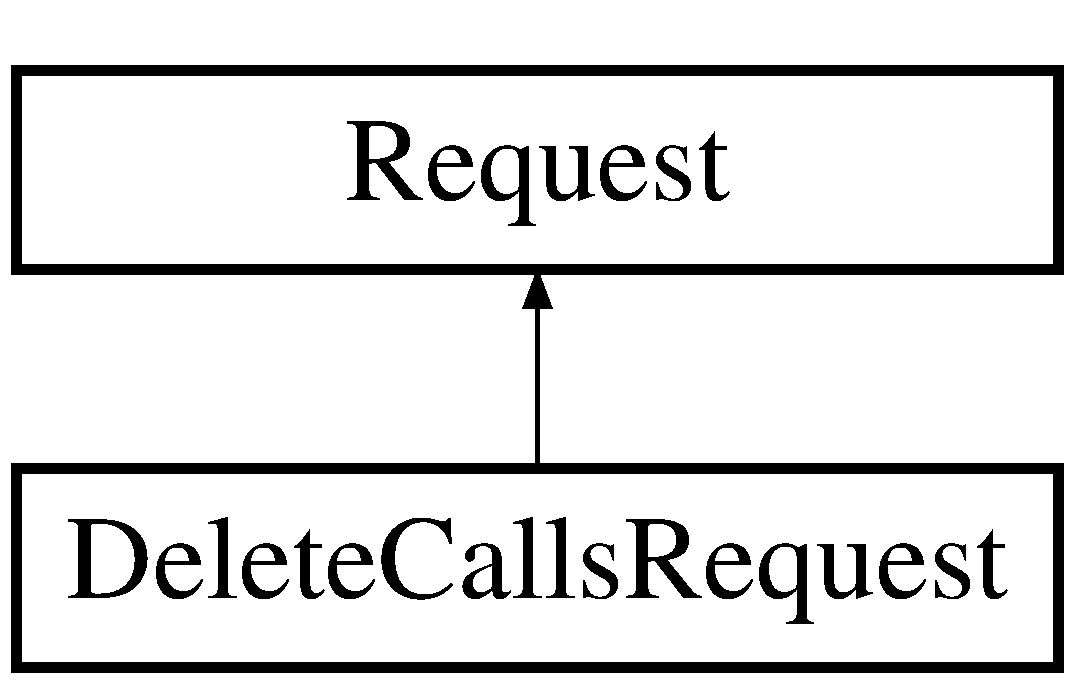
\includegraphics[height=2.000000cm]{class_delete_calls_request}
\end{center}
\end{figure}
\subsection*{Data Fields}
\begin{DoxyCompactItemize}
\item 
\hyperlink{class_delete_calls_request_a003384fac9231dcb79d5719b16e9eed8}{\$\-Ids}
\end{DoxyCompactItemize}


\subsection{Detailed Description}
The object sent for the \hyperlink{class_delete_calls_request}{Delete\-Calls\-Request} method 

\subsection{Field Documentation}
\hypertarget{class_delete_calls_request_a003384fac9231dcb79d5719b16e9eed8}{\index{Delete\-Calls\-Request@{Delete\-Calls\-Request}!\$\-Ids@{\$\-Ids}}
\index{\$\-Ids@{\$\-Ids}!DeleteCallsRequest@{Delete\-Calls\-Request}}
\subsubsection[{\$\-Ids}]{\setlength{\rightskip}{0pt plus 5cm}\$Ids}}\label{class_delete_calls_request_a003384fac9231dcb79d5719b16e9eed8}
array I\-Ds to delete 

The documentation for this class was generated from the following file\-:\begin{DoxyCompactItemize}
\item 
C\-:/\-Users/\-Jaime.\-Ushuaia/\-Documents/\-Git\-Hub/sleepy-\/mustache/include/class.\-robotalker.\-php\end{DoxyCompactItemize}

\hypertarget{class_filter}{\section{Filter Class Reference}
\label{class_filter}\index{Filter@{Filter}}
}
\subsection*{Public Member Functions}
\begin{DoxyCompactItemize}
\item 
\hyperlink{class_filter_a4717bbfc70a40a57ee741ed70766c309}{\-\_\-\-\_\-construct} (\$name)
\item 
\hyperlink{class_filter_a90cbfdb2d91157a1f2e94fcab3d220b3}{add} (\$function, \$args)
\end{DoxyCompactItemize}
\subsection*{Data Fields}
\begin{DoxyCompactItemize}
\item 
\hypertarget{class_filter_ab2fc40d43824ea3e1ce5d86dee0d763b}{{\bfseries \$name}}\label{class_filter_ab2fc40d43824ea3e1ce5d86dee0d763b}

\item 
\hyperlink{class_filter_aa75daea491817f3b64daa2f51128bcdf}{\$functions}
\end{DoxyCompactItemize}


\subsection{Detailed Description}
This class stores the filters. it has properties to store the name of the filter as well the functions that should run when the filters are stored. the filters property is an array. The key is the name of the function and value is the arguments. Currently we do not make any use of the arguments.


\begin{DoxyParams}[1]{Parameters}
string & {\em \$name} & name of the filter \\
\hline
\end{DoxyParams}
\begin{DoxyReturn}{Returns}
object 
\end{DoxyReturn}


\subsection{Constructor \& Destructor Documentation}
\hypertarget{class_filter_a4717bbfc70a40a57ee741ed70766c309}{\index{Filter@{Filter}!\-\_\-\-\_\-construct@{\-\_\-\-\_\-construct}}
\index{\-\_\-\-\_\-construct@{\-\_\-\-\_\-construct}!Filter@{Filter}}
\subsubsection[{\-\_\-\-\_\-construct}]{\setlength{\rightskip}{0pt plus 5cm}\-\_\-\-\_\-construct (
\begin{DoxyParamCaption}
\item[{}]{\$name}
\end{DoxyParamCaption}
)}}\label{class_filter_a4717bbfc70a40a57ee741ed70766c309}
Constructor 
\begin{DoxyParams}[1]{Parameters}
string & {\em \$name} & The name of the filter \\
\hline
\end{DoxyParams}


\subsection{Member Function Documentation}
\hypertarget{class_filter_a90cbfdb2d91157a1f2e94fcab3d220b3}{\index{Filter@{Filter}!add@{add}}
\index{add@{add}!Filter@{Filter}}
\subsubsection[{add}]{\setlength{\rightskip}{0pt plus 5cm}add (
\begin{DoxyParamCaption}
\item[{}]{\$function, }
\item[{}]{\$args}
\end{DoxyParamCaption}
)}}\label{class_filter_a90cbfdb2d91157a1f2e94fcab3d220b3}
Adds a function to this filter 
\begin{DoxyParams}[1]{Parameters}
string & {\em \$function} & The function to call \\
\hline
array & {\em \$args} & An array of parameters \\
\hline
\end{DoxyParams}


\subsection{Field Documentation}
\hypertarget{class_filter_aa75daea491817f3b64daa2f51128bcdf}{\index{Filter@{Filter}!\$functions@{\$functions}}
\index{\$functions@{\$functions}!Filter@{Filter}}
\subsubsection[{\$functions}]{\setlength{\rightskip}{0pt plus 5cm}\$functions}}\label{class_filter_aa75daea491817f3b64daa2f51128bcdf}
array a list of functions 

The documentation for this class was generated from the following file\-:\begin{DoxyCompactItemize}
\item 
C\-:/\-Users/\-Jaime.\-Ushuaia/\-Documents/\-Git\-Hub/sleepy-\/mustache/include/class.\-hooks.\-php\end{DoxyCompactItemize}

\hypertarget{class_f_s_d_b}{\section{F\-S\-D\-B Class Reference}
\label{class_f_s_d_b}\index{F\-S\-D\-B@{F\-S\-D\-B}}
}
\subsection*{Public Member Functions}
\begin{DoxyCompactItemize}
\item 
\hyperlink{class_f_s_d_b_a7e9ae789f3cd84fcb86ed612a20fd93f}{\-\_\-\-\_\-construct} (\$directory= '')
\item 
\hyperlink{class_f_s_d_b_a9f1179240d068c94a040021326032bed}{\-\_\-\-\_\-call} (\$method, \$args)
\end{DoxyCompactItemize}


\subsection{Detailed Description}
Filesystem Database\hypertarget{record1_dependencies}{}\subsection{Dependencies}\label{record1_dependencies}
class.\-F\-S\-Tables.\-php

\begin{DoxyAuthor}{Author}
Jaime A. Rodriguez \href{mailto:hi.i.am.jaime@gmail.com}{\tt hi.\-i.\-am.\-jaime@gmail.\-com} 
\end{DoxyAuthor}


\subsection{Constructor \& Destructor Documentation}
\hypertarget{class_f_s_d_b_a7e9ae789f3cd84fcb86ed612a20fd93f}{\index{F\-S\-D\-B@{F\-S\-D\-B}!\-\_\-\-\_\-construct@{\-\_\-\-\_\-construct}}
\index{\-\_\-\-\_\-construct@{\-\_\-\-\_\-construct}!FSDB@{F\-S\-D\-B}}
\subsubsection[{\-\_\-\-\_\-construct}]{\setlength{\rightskip}{0pt plus 5cm}\-\_\-\-\_\-construct (
\begin{DoxyParamCaption}
\item[{}]{\$directory = {\ttfamily ''}}
\end{DoxyParamCaption}
)}}\label{class_f_s_d_b_a7e9ae789f3cd84fcb86ed612a20fd93f}
\-\_\-\-\_\-construct


\begin{DoxyParams}[1]{Parameters}
string & {\em \$directory} & Directory where data is stored (optional) \\
\hline
\end{DoxyParams}


\subsection{Member Function Documentation}
\hypertarget{class_f_s_d_b_a9f1179240d068c94a040021326032bed}{\index{F\-S\-D\-B@{F\-S\-D\-B}!\-\_\-\-\_\-call@{\-\_\-\-\_\-call}}
\index{\-\_\-\-\_\-call@{\-\_\-\-\_\-call}!FSDB@{F\-S\-D\-B}}
\subsubsection[{\-\_\-\-\_\-call}]{\setlength{\rightskip}{0pt plus 5cm}\-\_\-\-\_\-call (
\begin{DoxyParamCaption}
\item[{}]{\$method, }
\item[{}]{\$args}
\end{DoxyParamCaption}
)}}\label{class_f_s_d_b_a9f1179240d068c94a040021326032bed}
\-\_\-\-\_\-call

Handles method calls, if the method exists in \hyperlink{class_f_s_table}{F\-S\-Table}, use that one.


\begin{DoxyParams}[1]{Parameters}
string & {\em \$method} & Method called \\
\hline
array & {\em \$args} & Arguments passed \\
\hline
\end{DoxyParams}
\begin{DoxyReturn}{Returns}
mixed Value. 
\end{DoxyReturn}


The documentation for this class was generated from the following file\-:\begin{DoxyCompactItemize}
\item 
C\-:/\-Users/\-Jaime.\-Ushuaia/\-Documents/\-Git\-Hub/sleepy-\/mustache/include/class.\-fsdb.\-php\end{DoxyCompactItemize}

\hypertarget{class_f_s_table}{\section{F\-S\-Table Class Reference}
\label{class_f_s_table}\index{F\-S\-Table@{F\-S\-Table}}
}
\subsection*{Public Member Functions}
\begin{DoxyCompactItemize}
\item 
\hyperlink{class_f_s_table_a8ef77288a5f940c68ebc57fdf0102078}{\-\_\-\-\_\-construct} (\$file)
\item 
\hyperlink{class_f_s_table_a421831a265621325e1fdd19aace0c758}{\-\_\-\-\_\-destruct} ()
\item 
\hyperlink{class_f_s_table_ad3d3dc4c1d2448d7b9f229448b57586a}{select} (\$column, \$search=0)
\item 
\hyperlink{class_f_s_table_ac3122ca1565ee89b1e4a1cb220960593}{select\-Range} (\$column, \$lower, \$upper)
\item 
\hyperlink{class_f_s_table_af8a4deeffdd08e76dce3d1083f729929}{update} (\$column, \$search=0, \$data=array())
\item 
\hyperlink{class_f_s_table_a2e355627d2f4a96559f022c4ab82df3c}{insert} (\$data)
\item 
\hyperlink{class_f_s_table_ac7aad87bd98f18250d97481375114759}{delete} (\$column, \$search=0)
\end{DoxyCompactItemize}


\subsection{Detailed Description}
Filesystem Table 

\subsection{Constructor \& Destructor Documentation}
\hypertarget{class_f_s_table_a8ef77288a5f940c68ebc57fdf0102078}{\index{F\-S\-Table@{F\-S\-Table}!\-\_\-\-\_\-construct@{\-\_\-\-\_\-construct}}
\index{\-\_\-\-\_\-construct@{\-\_\-\-\_\-construct}!FSTable@{F\-S\-Table}}
\subsubsection[{\-\_\-\-\_\-construct}]{\setlength{\rightskip}{0pt plus 5cm}\-\_\-\-\_\-construct (
\begin{DoxyParamCaption}
\item[{}]{\$file}
\end{DoxyParamCaption}
)}}\label{class_f_s_table_a8ef77288a5f940c68ebc57fdf0102078}
\-\_\-\-\_\-construct


\begin{DoxyParams}[1]{Parameters}
mixed & {\em \$file} & The file to open for this table. \\
\hline
\end{DoxyParams}
\hypertarget{class_f_s_table_a421831a265621325e1fdd19aace0c758}{\index{F\-S\-Table@{F\-S\-Table}!\-\_\-\-\_\-destruct@{\-\_\-\-\_\-destruct}}
\index{\-\_\-\-\_\-destruct@{\-\_\-\-\_\-destruct}!FSTable@{F\-S\-Table}}
\subsubsection[{\-\_\-\-\_\-destruct}]{\setlength{\rightskip}{0pt plus 5cm}\-\_\-\-\_\-destruct (
\begin{DoxyParamCaption}
{}
\end{DoxyParamCaption}
)}}\label{class_f_s_table_a421831a265621325e1fdd19aace0c758}
\-\_\-\-\_\-destruct 

\subsection{Member Function Documentation}
\hypertarget{class_f_s_table_ac7aad87bd98f18250d97481375114759}{\index{F\-S\-Table@{F\-S\-Table}!delete@{delete}}
\index{delete@{delete}!FSTable@{F\-S\-Table}}
\subsubsection[{delete}]{\setlength{\rightskip}{0pt plus 5cm}delete (
\begin{DoxyParamCaption}
\item[{}]{\$column, }
\item[{}]{\$search = {\ttfamily 0}}
\end{DoxyParamCaption}
)}}\label{class_f_s_table_ac7aad87bd98f18250d97481375114759}
Deletes rows from the table


\begin{DoxyParams}[1]{Parameters}
string & {\em \$column} & The column to match \\
\hline
mixed & {\em \$search} & What to search for \\
\hline
\end{DoxyParams}
\begin{DoxyReturn}{Returns}
int How many rows were deleted? 
\end{DoxyReturn}
\hypertarget{class_f_s_table_a2e355627d2f4a96559f022c4ab82df3c}{\index{F\-S\-Table@{F\-S\-Table}!insert@{insert}}
\index{insert@{insert}!FSTable@{F\-S\-Table}}
\subsubsection[{insert}]{\setlength{\rightskip}{0pt plus 5cm}insert (
\begin{DoxyParamCaption}
\item[{}]{\$data}
\end{DoxyParamCaption}
)}}\label{class_f_s_table_a2e355627d2f4a96559f022c4ab82df3c}
Inserts a new row into the table


\begin{DoxyParams}[1]{Parameters}
object & {\em \$data} & An object containing the row data. \\
\hline
\end{DoxyParams}
\begin{DoxyReturn}{Returns}
bool Was the operation successful? 
\end{DoxyReturn}
\hypertarget{class_f_s_table_ad3d3dc4c1d2448d7b9f229448b57586a}{\index{F\-S\-Table@{F\-S\-Table}!select@{select}}
\index{select@{select}!FSTable@{F\-S\-Table}}
\subsubsection[{select}]{\setlength{\rightskip}{0pt plus 5cm}select (
\begin{DoxyParamCaption}
\item[{}]{\$column, }
\item[{}]{\$search = {\ttfamily 0}}
\end{DoxyParamCaption}
)}}\label{class_f_s_table_ad3d3dc4c1d2448d7b9f229448b57586a}
Selects data from the table


\begin{DoxyParams}[1]{Parameters}
string & {\em \$column} & The column to match \\
\hline
mixed & {\em \$search} & What to search for \\
\hline
\end{DoxyParams}
\begin{DoxyReturn}{Returns}
array An array of rows in the form of objects. 
\end{DoxyReturn}
\hypertarget{class_f_s_table_ac3122ca1565ee89b1e4a1cb220960593}{\index{F\-S\-Table@{F\-S\-Table}!select\-Range@{select\-Range}}
\index{select\-Range@{select\-Range}!FSTable@{F\-S\-Table}}
\subsubsection[{select\-Range}]{\setlength{\rightskip}{0pt plus 5cm}select\-Range (
\begin{DoxyParamCaption}
\item[{}]{\$column, }
\item[{}]{\$lower, }
\item[{}]{\$upper}
\end{DoxyParamCaption}
)}}\label{class_f_s_table_ac3122ca1565ee89b1e4a1cb220960593}
Selects data from the table within a range


\begin{DoxyParams}[1]{Parameters}
string & {\em \$column} & The column to match \\
\hline
int & {\em \$lower} & The lower range \\
\hline
int & {\em \$upper} & The upper range \\
\hline
\end{DoxyParams}
\begin{DoxyReturn}{Returns}
array An array of rows in the form of objects. 
\end{DoxyReturn}
\hypertarget{class_f_s_table_af8a4deeffdd08e76dce3d1083f729929}{\index{F\-S\-Table@{F\-S\-Table}!update@{update}}
\index{update@{update}!FSTable@{F\-S\-Table}}
\subsubsection[{update}]{\setlength{\rightskip}{0pt plus 5cm}update (
\begin{DoxyParamCaption}
\item[{}]{\$column, }
\item[{}]{\$search = {\ttfamily 0}, }
\item[{}]{\$data = {\ttfamily array()}}
\end{DoxyParamCaption}
)}}\label{class_f_s_table_af8a4deeffdd08e76dce3d1083f729929}
Updates columns in the table.

Currently, it overwrites the whole row instead of merging the row.


\begin{DoxyParams}[1]{Parameters}
string & {\em \$column} & The column to match \\
\hline
mixed & {\em \$search} & What to search for \\
\hline
object & {\em \$data} & An object containing the row data. \\
\hline
\end{DoxyParams}
\begin{DoxyReturn}{Returns}
int How many rows were updated? 
\end{DoxyReturn}


The documentation for this class was generated from the following file\-:\begin{DoxyCompactItemize}
\item 
C\-:/\-Users/\-Jaime.\-Ushuaia/\-Documents/\-Git\-Hub/sleepy-\/mustache/modules/disabled/file-\/system-\/database/class.\-fsdb.\-php\end{DoxyCompactItemize}

\hypertarget{class_get_calls_request}{\section{Get\-Calls\-Request Class Reference}
\label{class_get_calls_request}\index{Get\-Calls\-Request@{Get\-Calls\-Request}}
}
Inheritance diagram for Get\-Calls\-Request\-:\begin{figure}[H]
\begin{center}
\leavevmode
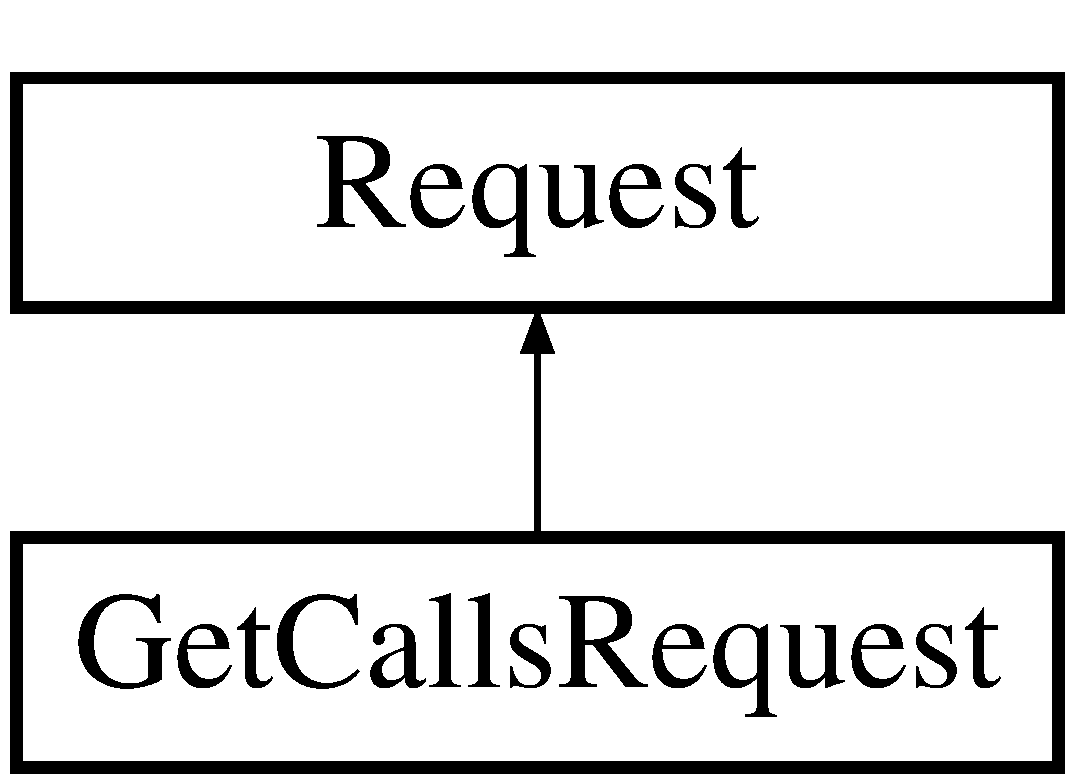
\includegraphics[height=2.000000cm]{class_get_calls_request}
\end{center}
\end{figure}
\subsection*{Data Fields}
\begin{DoxyCompactItemize}
\item 
\hyperlink{class_get_calls_request_a82e0539eeca49a1fbea42227a8f96d31}{\$\-Start\-Date}
\item 
\hyperlink{class_get_calls_request_a3ba74dcdb03b05077309a0b5a0c6788e}{\$\-End\-Date}
\end{DoxyCompactItemize}


\subsection{Detailed Description}
The object sent for the \hyperlink{class_get_calls_request}{Get\-Calls\-Request} method 

Definition at line 52 of file class.\-robotalker.\-php.



\subsection{Field Documentation}
\hypertarget{class_get_calls_request_a3ba74dcdb03b05077309a0b5a0c6788e}{\index{Get\-Calls\-Request@{Get\-Calls\-Request}!\$\-End\-Date@{\$\-End\-Date}}
\index{\$\-End\-Date@{\$\-End\-Date}!GetCallsRequest@{Get\-Calls\-Request}}
\subsubsection[{\$\-End\-Date}]{\setlength{\rightskip}{0pt plus 5cm}\$End\-Date}}\label{class_get_calls_request_a3ba74dcdb03b05077309a0b5a0c6788e}
Date\-Time The End Date 

Definition at line 61 of file class.\-robotalker.\-php.

\hypertarget{class_get_calls_request_a82e0539eeca49a1fbea42227a8f96d31}{\index{Get\-Calls\-Request@{Get\-Calls\-Request}!\$\-Start\-Date@{\$\-Start\-Date}}
\index{\$\-Start\-Date@{\$\-Start\-Date}!GetCallsRequest@{Get\-Calls\-Request}}
\subsubsection[{\$\-Start\-Date}]{\setlength{\rightskip}{0pt plus 5cm}\$Start\-Date}}\label{class_get_calls_request_a82e0539eeca49a1fbea42227a8f96d31}
Date\-Time The Start date 

Definition at line 56 of file class.\-robotalker.\-php.



The documentation for this class was generated from the following file\-:\begin{DoxyCompactItemize}
\item 
modules/disabled/robotalker/\hyperlink{class_8robotalker_8php}{class.\-robotalker.\-php}\end{DoxyCompactItemize}

\hypertarget{class_get_campaign_stats_request}{\section{Get\-Campaign\-Stats\-Request Class Reference}
\label{class_get_campaign_stats_request}\index{Get\-Campaign\-Stats\-Request@{Get\-Campaign\-Stats\-Request}}
}
Inheritance diagram for Get\-Campaign\-Stats\-Request\-:\begin{figure}[H]
\begin{center}
\leavevmode
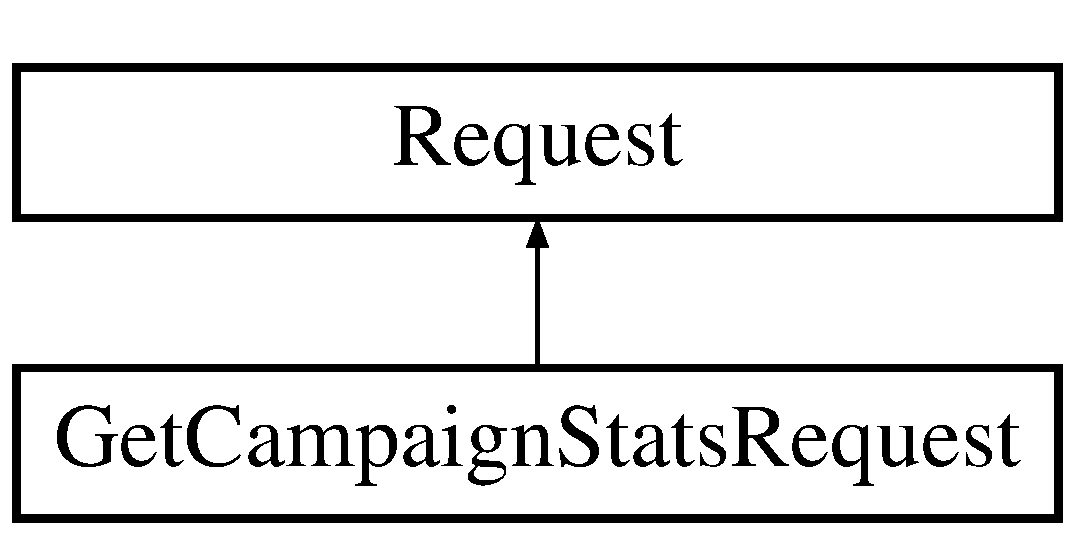
\includegraphics[height=2.000000cm]{class_get_campaign_stats_request}
\end{center}
\end{figure}
\subsection*{Public Member Functions}
\begin{DoxyCompactItemize}
\item 
\hyperlink{class_get_campaign_stats_request_a095c5d389db211932136b53f25f39685}{\-\_\-\-\_\-construct} ()
\end{DoxyCompactItemize}
\subsection*{Data Fields}
\begin{DoxyCompactItemize}
\item 
\hyperlink{class_get_campaign_stats_request_a2d22a3b5dcd66a7b8cc5db60947b5ca3}{\$\-Campaign\-Id}
\item 
\hyperlink{class_get_campaign_stats_request_a6a7dc0605d9a2e10066aeb57b77fc272}{\$\-Include\-Details}
\end{DoxyCompactItemize}


\subsection{Detailed Description}


Definition at line 67 of file class.\-robotalker.\-php.



\subsection{Constructor \& Destructor Documentation}
\hypertarget{class_get_campaign_stats_request_a095c5d389db211932136b53f25f39685}{\index{Get\-Campaign\-Stats\-Request@{Get\-Campaign\-Stats\-Request}!\-\_\-\-\_\-construct@{\-\_\-\-\_\-construct}}
\index{\-\_\-\-\_\-construct@{\-\_\-\-\_\-construct}!GetCampaignStatsRequest@{Get\-Campaign\-Stats\-Request}}
\subsubsection[{\-\_\-\-\_\-construct}]{\setlength{\rightskip}{0pt plus 5cm}\-\_\-\-\_\-construct (
\begin{DoxyParamCaption}
{}
\end{DoxyParamCaption}
)}}\label{class_get_campaign_stats_request_a095c5d389db211932136b53f25f39685}


Definition at line 74 of file class.\-robotalker.\-php.


\begin{DoxyCode}
                                             \{
                              $this->IncludeDetails = \textcolor{keyword}{true};
               \}
\end{DoxyCode}


\subsection{Field Documentation}
\hypertarget{class_get_campaign_stats_request_a2d22a3b5dcd66a7b8cc5db60947b5ca3}{\index{Get\-Campaign\-Stats\-Request@{Get\-Campaign\-Stats\-Request}!\$\-Campaign\-Id@{\$\-Campaign\-Id}}
\index{\$\-Campaign\-Id@{\$\-Campaign\-Id}!GetCampaignStatsRequest@{Get\-Campaign\-Stats\-Request}}
\subsubsection[{\$\-Campaign\-Id}]{\setlength{\rightskip}{0pt plus 5cm}\$Campaign\-Id}}\label{class_get_campaign_stats_request_a2d22a3b5dcd66a7b8cc5db60947b5ca3}
Int, The Campaign I\-D 

Definition at line 71 of file class.\-robotalker.\-php.

\hypertarget{class_get_campaign_stats_request_a6a7dc0605d9a2e10066aeb57b77fc272}{\index{Get\-Campaign\-Stats\-Request@{Get\-Campaign\-Stats\-Request}!\$\-Include\-Details@{\$\-Include\-Details}}
\index{\$\-Include\-Details@{\$\-Include\-Details}!GetCampaignStatsRequest@{Get\-Campaign\-Stats\-Request}}
\subsubsection[{\$\-Include\-Details}]{\setlength{\rightskip}{0pt plus 5cm}\$Include\-Details}}\label{class_get_campaign_stats_request_a6a7dc0605d9a2e10066aeb57b77fc272}


Definition at line 72 of file class.\-robotalker.\-php.



The documentation for this class was generated from the following file\-:\begin{DoxyCompactItemize}
\item 
modules/disabled/robotalker/\hyperlink{class_8robotalker_8php}{class.\-robotalker.\-php}\end{DoxyCompactItemize}

\hypertarget{class_hook}{\section{Hook Class Reference}
\label{class_hook}\index{Hook@{Hook}}
}
\subsection*{Static Public Member Functions}
\begin{DoxyCompactItemize}
\item 
static \hyperlink{class_hook_aae875eca0ec73f226ce615840f06d161}{apply\-Filter} (\$name, \$function, \$args='1')
\item 
static \hyperlink{class_hook_a6489ed6b12329279b9e7cae26afc4dd6}{add\-Filter} (\$name, \$value='')
\item 
static \hyperlink{class_hook_a044e40a84df383f73df2250624d13c42}{do\-Action} (\$name, \$function, \$args='1')
\item 
static \hyperlink{class_hook_afff7a7869d2dd304043b69a3fff24655}{add\-Action} (\$name)
\end{DoxyCompactItemize}
\subsection*{Static Public Attributes}
\begin{DoxyCompactItemize}
\item 
static \hyperlink{class_hook_aca1cfea95d9874525c94ddc586b87633}{\$directories}
\end{DoxyCompactItemize}


\subsection{Detailed Description}
This class is the main hook class. Call it using class\-::method. 
\begin{DoxyCode}
\hyperlink{class_hook_a6489ed6b12329279b9e7cae26afc4dd6}{Hook::addFilter}(\textcolor{stringliteral}{'fitername'}, $variable);
\end{DoxyCode}
 \begin{DoxyReturn}{Returns}
void 
\end{DoxyReturn}


Definition at line 80 of file class.\-hooks.\-php.



\subsection{Member Function Documentation}
\hypertarget{class_hook_afff7a7869d2dd304043b69a3fff24655}{\index{Hook@{Hook}!add\-Action@{add\-Action}}
\index{add\-Action@{add\-Action}!Hook@{Hook}}
\subsubsection[{add\-Action}]{\setlength{\rightskip}{0pt plus 5cm}static add\-Action (
\begin{DoxyParamCaption}
\item[{}]{\$name}
\end{DoxyParamCaption}
)\hspace{0.3cm}{\ttfamily [static]}}}\label{class_hook_afff7a7869d2dd304043b69a3fff24655}
Adds a new action-\/type hook point


\begin{DoxyParams}[1]{Parameters}
string & {\em \$name} & \mbox{[}description\mbox{]}\\
\hline
\end{DoxyParams}
\begin{DoxyReturn}{Returns}
void 
\end{DoxyReturn}


Definition at line 224 of file class.\-hooks.\-php.


\begin{DoxyCode}
                                                       \{
                              self::addFilter($name);
               \}
\end{DoxyCode}
\hypertarget{class_hook_a6489ed6b12329279b9e7cae26afc4dd6}{\index{Hook@{Hook}!add\-Filter@{add\-Filter}}
\index{add\-Filter@{add\-Filter}!Hook@{Hook}}
\subsubsection[{add\-Filter}]{\setlength{\rightskip}{0pt plus 5cm}static add\-Filter (
\begin{DoxyParamCaption}
\item[{}]{\$name, }
\item[{}]{\$value = {\ttfamily ''}}
\end{DoxyParamCaption}
)\hspace{0.3cm}{\ttfamily [static]}}}\label{class_hook_a6489ed6b12329279b9e7cae26afc4dd6}
Adds a new filter-\/type hook point


\begin{DoxyParams}[1]{Parameters}
mixed & {\em \$name} & \mbox{[}description\mbox{]} \\
\hline
string & {\em \$value} & \mbox{[}description\mbox{]}\\
\hline
\end{DoxyParams}
\begin{DoxyReturn}{Returns}
void 
\end{DoxyReturn}


Definition at line 183 of file class.\-hooks.\-php.


\begin{DoxyCode}
                                                                  \{
                              self::initialize();

                              \textcolor{keywordflow}{if} (!isset(self::$filters[$name])) \{
                                             \textcolor{keywordflow}{if} (is\_array($value)) \{
                                                            \textcolor{keywordflow}{return} $value[0];
                                             \} \textcolor{keywordflow}{else} \{
                                                            \textcolor{keywordflow}{return} $value;
                                             \}
                              \}

                              \textcolor{keywordflow}{foreach} (self::$filters[$name]->functions as 
      $function => $args) \{
                                             \textcolor{keywordflow}{if} (is\_array($value)) \{
                                                            $returned = 
      call\_user\_func\_array($function, $value);
                                             \} \textcolor{keywordflow}{else} \{
                                                            $returned = 
      call\_user\_func($function, $value);
                                             \}
                              \}

                              \textcolor{keywordflow}{return} $returned;
               \}
\end{DoxyCode}
\hypertarget{class_hook_aae875eca0ec73f226ce615840f06d161}{\index{Hook@{Hook}!apply\-Filter@{apply\-Filter}}
\index{apply\-Filter@{apply\-Filter}!Hook@{Hook}}
\subsubsection[{apply\-Filter}]{\setlength{\rightskip}{0pt plus 5cm}static apply\-Filter (
\begin{DoxyParamCaption}
\item[{}]{\$name, }
\item[{}]{\$function, }
\item[{}]{\$args = {\ttfamily '1'}}
\end{DoxyParamCaption}
)\hspace{0.3cm}{\ttfamily [static]}}}\label{class_hook_aae875eca0ec73f226ce615840f06d161}
Add a new filter to a filter-\/type hook point


\begin{DoxyParams}[1]{Parameters}
string & {\em \$name} & \mbox{[}description\mbox{]} \\
\hline
string & {\em \$function} & \mbox{[}description\mbox{]} \\
\hline
int & {\em \$args} & \mbox{[}description\mbox{]}\\
\hline
\end{DoxyParams}
\begin{DoxyReturn}{Returns}
void 
\end{DoxyReturn}


Definition at line 164 of file class.\-hooks.\-php.


\begin{DoxyCode}
                                                                               
      \{
                              self::initialize();

                              \textcolor{keywordflow}{if} (!isset(self::$filters[$name])) \{
                                             self::$filters[$name] = \textcolor{keyword}{new} \hyperlink{class_filter}{Filter}
       ($name);
                              \}

                              \textcolor{comment}{// add the function to the filter}
                              self::$filters[$name]->add($function, $args);
               \}
\end{DoxyCode}
\hypertarget{class_hook_a044e40a84df383f73df2250624d13c42}{\index{Hook@{Hook}!do\-Action@{do\-Action}}
\index{do\-Action@{do\-Action}!Hook@{Hook}}
\subsubsection[{do\-Action}]{\setlength{\rightskip}{0pt plus 5cm}static do\-Action (
\begin{DoxyParamCaption}
\item[{}]{\$name, }
\item[{}]{\$function, }
\item[{}]{\$args = {\ttfamily '1'}}
\end{DoxyParamCaption}
)\hspace{0.3cm}{\ttfamily [static]}}}\label{class_hook_a044e40a84df383f73df2250624d13c42}
Adds a new function to a action-\/type hook point


\begin{DoxyParams}[1]{Parameters}
string & {\em \$name} & Name of filter \\
\hline
string & {\em \$function} & Function to call\\
\hline
\end{DoxyParams}
\begin{DoxyReturn}{Returns}
void 
\end{DoxyReturn}


Definition at line 213 of file class.\-hooks.\-php.


\begin{DoxyCode}
                                                                            \{
                              self::applyFilter($name, $function, $args);
               \}
\end{DoxyCode}


\subsection{Field Documentation}
\hypertarget{class_hook_aca1cfea95d9874525c94ddc586b87633}{\index{Hook@{Hook}!\$directories@{\$directories}}
\index{\$directories@{\$directories}!Hook@{Hook}}
\subsubsection[{\$directories}]{\setlength{\rightskip}{0pt plus 5cm}\$directories\hspace{0.3cm}{\ttfamily [static]}}}\label{class_hook_aca1cfea95d9874525c94ddc586b87633}
array string The directories where the modules are stored 

Definition at line 97 of file class.\-hooks.\-php.



The documentation for this class was generated from the following file\-:\begin{DoxyCompactItemize}
\item 
include/\hyperlink{class_8hooks_8php}{class.\-hooks.\-php}\end{DoxyCompactItemize}

\hypertarget{class_i_p2_c_o}{\section{I\-P2\-C\-O Class Reference}
\label{class_i_p2_c_o}\index{I\-P2\-C\-O@{I\-P2\-C\-O}}
}
\subsection*{Public Member Functions}
\begin{DoxyCompactItemize}
\item 
\hypertarget{class_i_p2_c_o_a0aef1ce60812280445e63410f68f00a0}{{\bfseries get\-Country\-Code} (\$ip)}\label{class_i_p2_c_o_a0aef1ce60812280445e63410f68f00a0}

\item 
\hypertarget{class_i_p2_c_o_a827810b3e6446a9dd09e79a0d03f040d}{{\bfseries get\-Table} (\$ip)}\label{class_i_p2_c_o_a827810b3e6446a9dd09e79a0d03f040d}

\end{DoxyCompactItemize}


The documentation for this class was generated from the following file\-:\begin{DoxyCompactItemize}
\item 
C\-:/\-Users/\-Jaime.\-Ushuaia/\-Documents/\-Git\-Hub/sleepy-\/mustache/include/class.\-ip2country.\-php\end{DoxyCompactItemize}

\hypertarget{class_login_request}{\section{Login\-Request Class Reference}
\label{class_login_request}\index{Login\-Request@{Login\-Request}}
}
Inheritance diagram for Login\-Request\-:\begin{figure}[H]
\begin{center}
\leavevmode
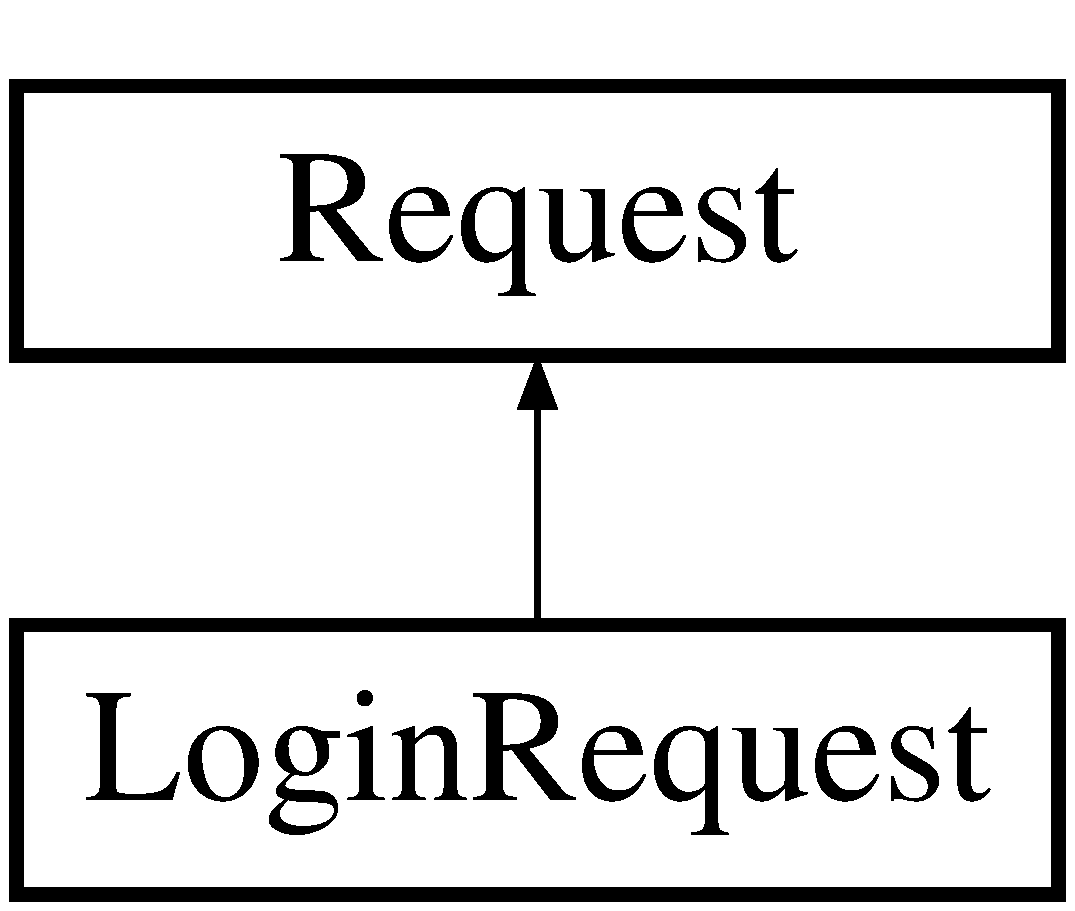
\includegraphics[height=2.000000cm]{class_login_request}
\end{center}
\end{figure}
\subsection*{Data Fields}
\begin{DoxyCompactItemize}
\item 
\hyperlink{class_login_request_a5e6181896c4104715348824d02a3075d}{\$\-User\-Id}
\item 
\hyperlink{class_login_request_ae3ac8512c0fd8924c7112671ead08cf7}{\$\-Password}
\end{DoxyCompactItemize}


\subsection{Detailed Description}
The object sent for the \hyperlink{class_login_request}{Login\-Request} method 

Definition at line 37 of file class.\-robotalker.\-php.



\subsection{Field Documentation}
\hypertarget{class_login_request_ae3ac8512c0fd8924c7112671ead08cf7}{\index{Login\-Request@{Login\-Request}!\$\-Password@{\$\-Password}}
\index{\$\-Password@{\$\-Password}!LoginRequest@{Login\-Request}}
\subsubsection[{\$\-Password}]{\setlength{\rightskip}{0pt plus 5cm}\$Password}}\label{class_login_request_ae3ac8512c0fd8924c7112671ead08cf7}
String Password for the \hyperlink{class_user}{User} 

Definition at line 46 of file class.\-robotalker.\-php.

\hypertarget{class_login_request_a5e6181896c4104715348824d02a3075d}{\index{Login\-Request@{Login\-Request}!\$\-User\-Id@{\$\-User\-Id}}
\index{\$\-User\-Id@{\$\-User\-Id}!LoginRequest@{Login\-Request}}
\subsubsection[{\$\-User\-Id}]{\setlength{\rightskip}{0pt plus 5cm}\$User\-Id}}\label{class_login_request_a5e6181896c4104715348824d02a3075d}
String \hyperlink{class_user}{User} I\-D of the Login \hyperlink{class_request}{Request} 

Definition at line 41 of file class.\-robotalker.\-php.



The documentation for this class was generated from the following file\-:\begin{DoxyCompactItemize}
\item 
modules/disabled/robotalker/\hyperlink{class_8robotalker_8php}{class.\-robotalker.\-php}\end{DoxyCompactItemize}

\hypertarget{class_mailer}{\section{Mailer Class Reference}
\label{class_mailer}\index{Mailer@{Mailer}}
}
\subsection*{Public Member Functions}
\begin{DoxyCompactItemize}
\item 
\hyperlink{class_mailer_a12bcef5130168b80d3d52dc82213f19a}{send} ()
\item 
\hyperlink{class_mailer_aacb4d359fe0baad6a39ebda1613f1b3a}{add\-To} (\$email)
\item 
\hyperlink{class_mailer_a36316da1ac12624e7817cbc65ba51726}{add\-Cc} (\$email)
\item 
\hyperlink{class_mailer_ac320ba7834972b0109bec4627f18122a}{add\-Bcc} (\$email)
\item 
\hyperlink{class_mailer_a94bb8db8b58c3919ef8fcf714c217d30}{add\-From} (\$email)
\item 
\hyperlink{class_mailer_a305e6eb17fe7d49383d9ddeb57ea54be}{fetch\-Html} (\$url)
\item 
\hyperlink{class_mailer_aa8ccfd30329dbb3cd1b5740173072c9e}{msg\-Text} (\$msg, \$switch=false)
\item 
\hyperlink{class_mailer_afca153730fe26e45a98e1540f20b69f2}{add\-Subject} (\$subject='')
\end{DoxyCompactItemize}


\subsection{Member Function Documentation}
\hypertarget{class_mailer_ac320ba7834972b0109bec4627f18122a}{\index{Mailer@{Mailer}!add\-Bcc@{add\-Bcc}}
\index{add\-Bcc@{add\-Bcc}!Mailer@{Mailer}}
\subsubsection[{add\-Bcc}]{\setlength{\rightskip}{0pt plus 5cm}add\-Bcc (
\begin{DoxyParamCaption}
\item[{}]{\$email}
\end{DoxyParamCaption}
)}}\label{class_mailer_ac320ba7834972b0109bec4627f18122a}
Adds a Blind Carbon Copy recipient. 
\begin{DoxyParams}[1]{Parameters}
string & {\em \$email} & A valid email address \\
\hline
\end{DoxyParams}
\hypertarget{class_mailer_a36316da1ac12624e7817cbc65ba51726}{\index{Mailer@{Mailer}!add\-Cc@{add\-Cc}}
\index{add\-Cc@{add\-Cc}!Mailer@{Mailer}}
\subsubsection[{add\-Cc}]{\setlength{\rightskip}{0pt plus 5cm}add\-Cc (
\begin{DoxyParamCaption}
\item[{}]{\$email}
\end{DoxyParamCaption}
)}}\label{class_mailer_a36316da1ac12624e7817cbc65ba51726}
Adds a Carbon Copy recipient. 
\begin{DoxyParams}[1]{Parameters}
string & {\em \$email} & A valid email address. \\
\hline
\end{DoxyParams}
\hypertarget{class_mailer_a94bb8db8b58c3919ef8fcf714c217d30}{\index{Mailer@{Mailer}!add\-From@{add\-From}}
\index{add\-From@{add\-From}!Mailer@{Mailer}}
\subsubsection[{add\-From}]{\setlength{\rightskip}{0pt plus 5cm}add\-From (
\begin{DoxyParamCaption}
\item[{}]{\$email}
\end{DoxyParamCaption}
)}}\label{class_mailer_a94bb8db8b58c3919ef8fcf714c217d30}
Sets a senders email address. 
\begin{DoxyParams}[1]{Parameters}
string & {\em \$email} & A valid email address. \\
\hline
\end{DoxyParams}
\hypertarget{class_mailer_afca153730fe26e45a98e1540f20b69f2}{\index{Mailer@{Mailer}!add\-Subject@{add\-Subject}}
\index{add\-Subject@{add\-Subject}!Mailer@{Mailer}}
\subsubsection[{add\-Subject}]{\setlength{\rightskip}{0pt plus 5cm}add\-Subject (
\begin{DoxyParamCaption}
\item[{}]{\$subject = {\ttfamily ''}}
\end{DoxyParamCaption}
)}}\label{class_mailer_afca153730fe26e45a98e1540f20b69f2}
Adds a subject to the email. If there is no subject the time will be used. 
\begin{DoxyParams}[1]{Parameters}
string & {\em \$subject} & The subject of the email \\
\hline
\end{DoxyParams}
\hypertarget{class_mailer_aacb4d359fe0baad6a39ebda1613f1b3a}{\index{Mailer@{Mailer}!add\-To@{add\-To}}
\index{add\-To@{add\-To}!Mailer@{Mailer}}
\subsubsection[{add\-To}]{\setlength{\rightskip}{0pt plus 5cm}add\-To (
\begin{DoxyParamCaption}
\item[{}]{\$email}
\end{DoxyParamCaption}
)}}\label{class_mailer_aacb4d359fe0baad6a39ebda1613f1b3a}
Adds a primary recipient.


\begin{DoxyParams}[1]{Parameters}
string & {\em \$email} & A valid email address. \\
\hline
\end{DoxyParams}
\hypertarget{class_mailer_a305e6eb17fe7d49383d9ddeb57ea54be}{\index{Mailer@{Mailer}!fetch\-Html@{fetch\-Html}}
\index{fetch\-Html@{fetch\-Html}!Mailer@{Mailer}}
\subsubsection[{fetch\-Html}]{\setlength{\rightskip}{0pt plus 5cm}fetch\-Html (
\begin{DoxyParamCaption}
\item[{}]{\$url}
\end{DoxyParamCaption}
)}}\label{class_mailer_a305e6eb17fe7d49383d9ddeb57ea54be}
Gets H\-T\-M\-L for a \$url and repalces anything in the body of the email with the H\-T\-M\-L that it fetched. 
\begin{DoxyParams}[1]{Parameters}
string & {\em \$url} & the url of an html file for the email body. \\
\hline
\end{DoxyParams}
\hypertarget{class_mailer_aa8ccfd30329dbb3cd1b5740173072c9e}{\index{Mailer@{Mailer}!msg\-Text@{msg\-Text}}
\index{msg\-Text@{msg\-Text}!Mailer@{Mailer}}
\subsubsection[{msg\-Text}]{\setlength{\rightskip}{0pt plus 5cm}msg\-Text (
\begin{DoxyParamCaption}
\item[{}]{\$msg, }
\item[{}]{\$switch = {\ttfamily false}}
\end{DoxyParamCaption}
)}}\label{class_mailer_aa8ccfd30329dbb3cd1b5740173072c9e}
Sets the body of the email to text. 
\begin{DoxyParams}[1]{Parameters}
string & {\em \$msg} & a string for the body \\
\hline
boolean & {\em \$switch} & an optional parameter for overloading \$this-\/$>$html \\
\hline
\end{DoxyParams}
\hypertarget{class_mailer_a12bcef5130168b80d3d52dc82213f19a}{\index{Mailer@{Mailer}!send@{send}}
\index{send@{send}!Mailer@{Mailer}}
\subsubsection[{send}]{\setlength{\rightskip}{0pt plus 5cm}send (
\begin{DoxyParamCaption}
{}
\end{DoxyParamCaption}
)}}\label{class_mailer_a12bcef5130168b80d3d52dc82213f19a}
Sends the email.

\begin{DoxyReturn}{Returns}
bool Was the email successfully sent? 
\end{DoxyReturn}


The documentation for this class was generated from the following file\-:\begin{DoxyCompactItemize}
\item 
C\-:/\-Users/\-Jaime.\-Ushuaia/\-Documents/\-Git\-Hub/sleepy-\/mustache/modules/disabled/mailer/class.\-mailer.\-php\end{DoxyCompactItemize}

\hypertarget{class_message_recipient_of_int32}{\section{Message\-Recipient\-Of\-Int32 Class Reference}
\label{class_message_recipient_of_int32}\index{Message\-Recipient\-Of\-Int32@{Message\-Recipient\-Of\-Int32}}
}
\subsection*{Data Fields}
\begin{DoxyCompactItemize}
\item 
\hyperlink{class_message_recipient_of_int32_a80e5e7a3e0698eb7784c0251e40b8077}{\$\-Dial\-Number}
\end{DoxyCompactItemize}


\subsection{Detailed Description}
Recipeient used in Schedule\-Calls 

\subsection{Field Documentation}
\hypertarget{class_message_recipient_of_int32_a80e5e7a3e0698eb7784c0251e40b8077}{\index{Message\-Recipient\-Of\-Int32@{Message\-Recipient\-Of\-Int32}!\$\-Dial\-Number@{\$\-Dial\-Number}}
\index{\$\-Dial\-Number@{\$\-Dial\-Number}!MessageRecipientOfInt32@{Message\-Recipient\-Of\-Int32}}
\subsubsection[{\$\-Dial\-Number}]{\setlength{\rightskip}{0pt plus 5cm}\$Dial\-Number}}\label{class_message_recipient_of_int32_a80e5e7a3e0698eb7784c0251e40b8077}
String Optional. Recipient Name String Phone number to send message to 

The documentation for this class was generated from the following file\-:\begin{DoxyCompactItemize}
\item 
C\-:/\-Users/\-Jaime.\-Ushuaia/\-Documents/\-Git\-Hub/sleepy-\/mustache/modules/disabled/robotalker/class.\-robotalker.\-php\end{DoxyCompactItemize}

\hypertarget{class_mobi_detect}{\section{Mobi\-Detect Class Reference}
\label{class_mobi_detect}\index{Mobi\-Detect@{Mobi\-Detect}}
}
\subsection*{Public Member Functions}
\begin{DoxyCompactItemize}
\item 
\hyperlink{class_mobi_detect_a095c5d389db211932136b53f25f39685}{\-\_\-\-\_\-construct} ()
\item 
\hyperlink{class_mobi_detect_aa03affe506ea70c6d04fab89fee473fc}{is\-Mobile} ()
\item 
\hyperlink{class_mobi_detect_abef4c1a6a8052c28a3c2dec49d3f9e9b}{is\-Iphone} ()
\item 
\hyperlink{class_mobi_detect_a2d202f72c3038ed6852aebff550dc531}{is\-Ipad} ()
\item 
\hyperlink{class_mobi_detect_abcbe8c4d1560467d47a8e19fe4554c85}{is\-Android} ()
\item 
\hyperlink{class_mobi_detect_a8a2049e411c252249d5264f87f2a894c}{is\-Opera} ()
\item 
\hyperlink{class_mobi_detect_a5eea8483425fa1d463e9df4b9e6f955b}{is\-Blackberry} ()
\item 
\hyperlink{class_mobi_detect_a1342be6bfbf8c34d00c89b8a880ac61e}{is\-Palm} ()
\item 
\hyperlink{class_mobi_detect_abd0a3ffcb33cbef4d23adbede9e3fcd4}{is\-Windows\-Phone} ()
\end{DoxyCompactItemize}


\subsection{Detailed Description}
Detects if a device is a mobile device and which kind.

Attribution\-: Regex taken from unknown source

\begin{DoxyAuthor}{Author}
Jaime A. Rodriguez \href{mailto:hi.i.am.jaime@gmail.com}{\tt hi.\-i.\-am.\-jaime@gmail.\-com} 
\end{DoxyAuthor}
\begin{DoxyVersion}{Version}
1.\-0 
\end{DoxyVersion}
\begin{DoxyCopyright}{Copyright}
G\-P\-L 3 \href{http://cuttingedgecode.com}{\tt http\-://cuttingedgecode.\-com} 
\end{DoxyCopyright}


Definition at line 12 of file class.\-mobidetect.\-php.



\subsection{Constructor \& Destructor Documentation}
\hypertarget{class_mobi_detect_a095c5d389db211932136b53f25f39685}{\index{Mobi\-Detect@{Mobi\-Detect}!\-\_\-\-\_\-construct@{\-\_\-\-\_\-construct}}
\index{\-\_\-\-\_\-construct@{\-\_\-\-\_\-construct}!MobiDetect@{Mobi\-Detect}}
\subsubsection[{\-\_\-\-\_\-construct}]{\setlength{\rightskip}{0pt plus 5cm}\-\_\-\-\_\-construct (
\begin{DoxyParamCaption}
{}
\end{DoxyParamCaption}
)}}\label{class_mobi_detect_a095c5d389db211932136b53f25f39685}


Definition at line 22 of file class.\-mobidetect.\-php.


\begin{DoxyCode}
                                             \{
                              $this->detect();
               \}
\end{DoxyCode}


\subsection{Member Function Documentation}
\hypertarget{class_mobi_detect_abcbe8c4d1560467d47a8e19fe4554c85}{\index{Mobi\-Detect@{Mobi\-Detect}!is\-Android@{is\-Android}}
\index{is\-Android@{is\-Android}!MobiDetect@{Mobi\-Detect}}
\subsubsection[{is\-Android}]{\setlength{\rightskip}{0pt plus 5cm}is\-Android (
\begin{DoxyParamCaption}
{}
\end{DoxyParamCaption}
)}}\label{class_mobi_detect_abcbe8c4d1560467d47a8e19fe4554c85}
Checks if it is an Android

\begin{DoxyReturn}{Returns}
bool True if device is an Android. 
\end{DoxyReturn}


Definition at line 113 of file class.\-mobidetect.\-php.


\begin{DoxyCode}
                                           \{
                              \textcolor{keywordflow}{return} $this->android;
               \}
\end{DoxyCode}
\hypertarget{class_mobi_detect_a5eea8483425fa1d463e9df4b9e6f955b}{\index{Mobi\-Detect@{Mobi\-Detect}!is\-Blackberry@{is\-Blackberry}}
\index{is\-Blackberry@{is\-Blackberry}!MobiDetect@{Mobi\-Detect}}
\subsubsection[{is\-Blackberry}]{\setlength{\rightskip}{0pt plus 5cm}is\-Blackberry (
\begin{DoxyParamCaption}
{}
\end{DoxyParamCaption}
)}}\label{class_mobi_detect_a5eea8483425fa1d463e9df4b9e6f955b}
Checks if it is a Blackberry

\begin{DoxyReturn}{Returns}
bool True if device is a Blackberry. 
\end{DoxyReturn}


Definition at line 135 of file class.\-mobidetect.\-php.


\begin{DoxyCode}
                                              \{
                              \textcolor{keywordflow}{return} $this->blackberry;
               \}
\end{DoxyCode}
\hypertarget{class_mobi_detect_a2d202f72c3038ed6852aebff550dc531}{\index{Mobi\-Detect@{Mobi\-Detect}!is\-Ipad@{is\-Ipad}}
\index{is\-Ipad@{is\-Ipad}!MobiDetect@{Mobi\-Detect}}
\subsubsection[{is\-Ipad}]{\setlength{\rightskip}{0pt plus 5cm}is\-Ipad (
\begin{DoxyParamCaption}
{}
\end{DoxyParamCaption}
)}}\label{class_mobi_detect_a2d202f72c3038ed6852aebff550dc531}
Checks if it is an i\-Pad

\begin{DoxyReturn}{Returns}
bool True if device is an i\-Pad. 
\end{DoxyReturn}


Definition at line 102 of file class.\-mobidetect.\-php.


\begin{DoxyCode}
                                        \{
                              \textcolor{keywordflow}{return} $this->ipad;
               \}
\end{DoxyCode}
\hypertarget{class_mobi_detect_abef4c1a6a8052c28a3c2dec49d3f9e9b}{\index{Mobi\-Detect@{Mobi\-Detect}!is\-Iphone@{is\-Iphone}}
\index{is\-Iphone@{is\-Iphone}!MobiDetect@{Mobi\-Detect}}
\subsubsection[{is\-Iphone}]{\setlength{\rightskip}{0pt plus 5cm}is\-Iphone (
\begin{DoxyParamCaption}
{}
\end{DoxyParamCaption}
)}}\label{class_mobi_detect_abef4c1a6a8052c28a3c2dec49d3f9e9b}
Checks if it is an i\-Phone

\begin{DoxyReturn}{Returns}
bool True if device is an i\-Phone. 
\end{DoxyReturn}


Definition at line 91 of file class.\-mobidetect.\-php.


\begin{DoxyCode}
                                          \{
                              \textcolor{keywordflow}{return} $this->iphone;
               \}
\end{DoxyCode}
\hypertarget{class_mobi_detect_aa03affe506ea70c6d04fab89fee473fc}{\index{Mobi\-Detect@{Mobi\-Detect}!is\-Mobile@{is\-Mobile}}
\index{is\-Mobile@{is\-Mobile}!MobiDetect@{Mobi\-Detect}}
\subsubsection[{is\-Mobile}]{\setlength{\rightskip}{0pt plus 5cm}is\-Mobile (
\begin{DoxyParamCaption}
{}
\end{DoxyParamCaption}
)}}\label{class_mobi_detect_aa03affe506ea70c6d04fab89fee473fc}
Checks if it is a mobile device.

\begin{DoxyReturn}{Returns}
bool True if device is mobile. 
\end{DoxyReturn}


Definition at line 80 of file class.\-mobidetect.\-php.


\begin{DoxyCode}
                                          \{
                              \textcolor{keywordflow}{return} $this->mobileBrowser;
               \}
\end{DoxyCode}
\hypertarget{class_mobi_detect_a8a2049e411c252249d5264f87f2a894c}{\index{Mobi\-Detect@{Mobi\-Detect}!is\-Opera@{is\-Opera}}
\index{is\-Opera@{is\-Opera}!MobiDetect@{Mobi\-Detect}}
\subsubsection[{is\-Opera}]{\setlength{\rightskip}{0pt plus 5cm}is\-Opera (
\begin{DoxyParamCaption}
{}
\end{DoxyParamCaption}
)}}\label{class_mobi_detect_a8a2049e411c252249d5264f87f2a894c}
Checks if the browser is Opera Mini

\begin{DoxyReturn}{Returns}
bool True if browser is Opera Mini 
\end{DoxyReturn}


Definition at line 124 of file class.\-mobidetect.\-php.


\begin{DoxyCode}
                                         \{
                              \textcolor{keywordflow}{return} $this->opera;
               \}
\end{DoxyCode}
\hypertarget{class_mobi_detect_a1342be6bfbf8c34d00c89b8a880ac61e}{\index{Mobi\-Detect@{Mobi\-Detect}!is\-Palm@{is\-Palm}}
\index{is\-Palm@{is\-Palm}!MobiDetect@{Mobi\-Detect}}
\subsubsection[{is\-Palm}]{\setlength{\rightskip}{0pt plus 5cm}is\-Palm (
\begin{DoxyParamCaption}
{}
\end{DoxyParamCaption}
)}}\label{class_mobi_detect_a1342be6bfbf8c34d00c89b8a880ac61e}
Checks if it is a Palm device

\begin{DoxyReturn}{Returns}
bool True if device is a Palm device. 
\end{DoxyReturn}


Definition at line 146 of file class.\-mobidetect.\-php.


\begin{DoxyCode}
                                        \{
                              \textcolor{keywordflow}{return} $this->palm;
               \}
\end{DoxyCode}
\hypertarget{class_mobi_detect_abd0a3ffcb33cbef4d23adbede9e3fcd4}{\index{Mobi\-Detect@{Mobi\-Detect}!is\-Windows\-Phone@{is\-Windows\-Phone}}
\index{is\-Windows\-Phone@{is\-Windows\-Phone}!MobiDetect@{Mobi\-Detect}}
\subsubsection[{is\-Windows\-Phone}]{\setlength{\rightskip}{0pt plus 5cm}is\-Windows\-Phone (
\begin{DoxyParamCaption}
{}
\end{DoxyParamCaption}
)}}\label{class_mobi_detect_abd0a3ffcb33cbef4d23adbede9e3fcd4}
Checks if it is a Windows Phone

\begin{DoxyReturn}{Returns}
bool True if device is a Windows Phone. 
\end{DoxyReturn}


Definition at line 157 of file class.\-mobidetect.\-php.


\begin{DoxyCode}
                                                \{
                              \textcolor{keywordflow}{return} $this->windowsPhone;
               \}
\end{DoxyCode}


The documentation for this class was generated from the following file\-:\begin{DoxyCompactItemize}
\item 
modules/disabled/mobile-\/detection/\hyperlink{class_8mobidetect_8php}{class.\-mobidetect.\-php}\end{DoxyCompactItemize}

\hypertarget{class_navigation}{\section{Navigation Class Reference}
\label{class_navigation}\index{Navigation@{Navigation}}
}
\subsection*{Public Member Functions}
\begin{DoxyCompactItemize}
\item 
\hyperlink{class_navigation_a71b24a14f528d85045f4fcb455bf246f}{\-\_\-\-\_\-construct} (\$json='')
\item 
\hyperlink{class_navigation_a8959f1f09ce2d2b6ee6f8d2f28eec323}{show} (\$class=\char`\"{}\char`\"{})
\item 
\hyperlink{class_navigation_adb328aaddf2eb1f953bb026ef25094e7}{set\-Current} (\$string)
\end{DoxyCompactItemize}


\subsection{Detailed Description}


Definition at line 50 of file class.\-navigation.\-php.



\subsection{Constructor \& Destructor Documentation}
\hypertarget{class_navigation_a71b24a14f528d85045f4fcb455bf246f}{\index{Navigation@{Navigation}!\-\_\-\-\_\-construct@{\-\_\-\-\_\-construct}}
\index{\-\_\-\-\_\-construct@{\-\_\-\-\_\-construct}!Navigation@{Navigation}}
\subsubsection[{\-\_\-\-\_\-construct}]{\setlength{\rightskip}{0pt plus 5cm}\-\_\-\-\_\-construct (
\begin{DoxyParamCaption}
\item[{}]{\$json = {\ttfamily ''}}
\end{DoxyParamCaption}
)}}\label{class_navigation_a71b24a14f528d85045f4fcb455bf246f}
Constructor 
\begin{DoxyParams}[1]{Parameters}
string & {\em \$json} & json data containing the \hyperlink{class_navigation}{Navigation} data \\
\hline
\end{DoxyParams}


Definition at line 66 of file class.\-navigation.\-php.



\subsection{Member Function Documentation}
\hypertarget{class_navigation_adb328aaddf2eb1f953bb026ef25094e7}{\index{Navigation@{Navigation}!set\-Current@{set\-Current}}
\index{set\-Current@{set\-Current}!Navigation@{Navigation}}
\subsubsection[{set\-Current}]{\setlength{\rightskip}{0pt plus 5cm}set\-Current (
\begin{DoxyParamCaption}
\item[{}]{\$string}
\end{DoxyParamCaption}
)}}\label{class_navigation_adb328aaddf2eb1f953bb026ef25094e7}
Sets the current page search string 
\begin{DoxyParams}[1]{Parameters}
string & {\em \$string} & A string used to determine if a page is current \\
\hline
\end{DoxyParams}


Definition at line 147 of file class.\-navigation.\-php.

\hypertarget{class_navigation_a8959f1f09ce2d2b6ee6f8d2f28eec323}{\index{Navigation@{Navigation}!show@{show}}
\index{show@{show}!Navigation@{Navigation}}
\subsubsection[{show}]{\setlength{\rightskip}{0pt plus 5cm}show (
\begin{DoxyParamCaption}
\item[{}]{\$class = {\ttfamily \char`\"{}\char`\"{}}}
\end{DoxyParamCaption}
)}}\label{class_navigation_a8959f1f09ce2d2b6ee6f8d2f28eec323}
Renders the \hyperlink{class_navigation}{Navigation} \begin{DoxyReturn}{Returns}
string The rendered navigation 
\end{DoxyReturn}


Definition at line 139 of file class.\-navigation.\-php.



The documentation for this class was generated from the following file\-:\begin{DoxyCompactItemize}
\item 
modules/enabled/navigation/\hyperlink{class_8navigation_8php}{class.\-navigation.\-php}\end{DoxyCompactItemize}

\hypertarget{class_performance}{\section{Performance Class Reference}
\label{class_performance}\index{Performance@{Performance}}
}
\subsection*{Static Public Member Functions}
\begin{DoxyCompactItemize}
\item 
static \hyperlink{class_performance_a1f9e601dc116eccc60485bab6079b705}{start} (\$label)
\item 
static \hyperlink{class_performance_aede39ba61c77f5b8458f3fcaafe48ab9}{stop} (\$label)
\end{DoxyCompactItemize}


\subsection{Detailed Description}


Definition at line 27 of file class.\-performance.\-php.



\subsection{Member Function Documentation}
\hypertarget{class_performance_a1f9e601dc116eccc60485bab6079b705}{\index{Performance@{Performance}!start@{start}}
\index{start@{start}!Performance@{Performance}}
\subsubsection[{start}]{\setlength{\rightskip}{0pt plus 5cm}static start (
\begin{DoxyParamCaption}
\item[{}]{\$label}
\end{DoxyParamCaption}
)\hspace{0.3cm}{\ttfamily [static]}}}\label{class_performance_a1f9e601dc116eccc60485bab6079b705}


Definition at line 30 of file class.\-performance.\-php.

\hypertarget{class_performance_aede39ba61c77f5b8458f3fcaafe48ab9}{\index{Performance@{Performance}!stop@{stop}}
\index{stop@{stop}!Performance@{Performance}}
\subsubsection[{stop}]{\setlength{\rightskip}{0pt plus 5cm}static stop (
\begin{DoxyParamCaption}
\item[{}]{\$label}
\end{DoxyParamCaption}
)\hspace{0.3cm}{\ttfamily [static]}}}\label{class_performance_aede39ba61c77f5b8458f3fcaafe48ab9}


Definition at line 34 of file class.\-performance.\-php.



The documentation for this class was generated from the following file\-:\begin{DoxyCompactItemize}
\item 
include/\hyperlink{class_8performance_8php}{class.\-performance.\-php}\end{DoxyCompactItemize}

\hypertarget{class_permission}{\section{Permission Class Reference}
\label{class_permission}\index{Permission@{Permission}}
}
Inheritance diagram for Permission\-:\begin{figure}[H]
\begin{center}
\leavevmode
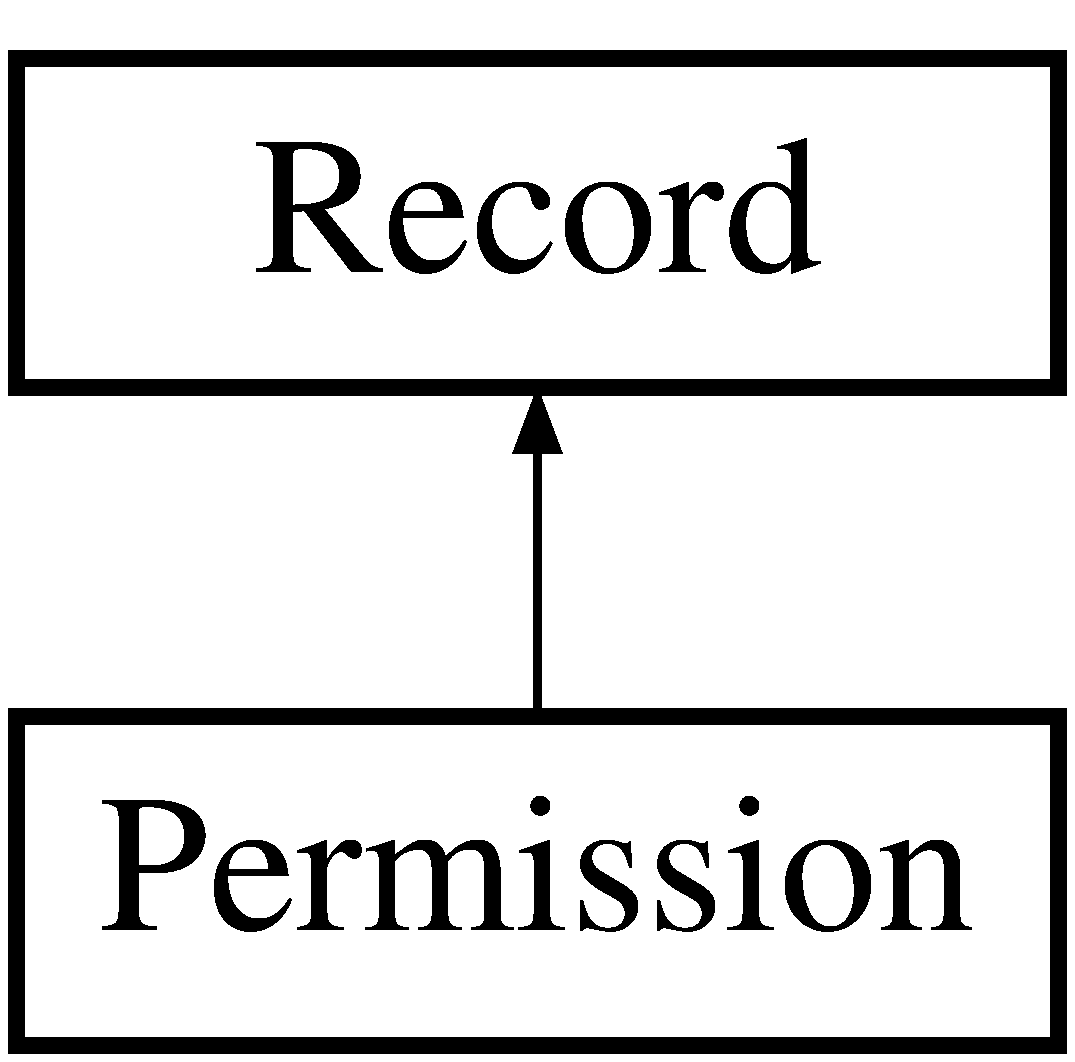
\includegraphics[height=2.000000cm]{class_permission}
\end{center}
\end{figure}
\subsection*{Data Fields}
\begin{DoxyCompactItemize}
\item 
\hypertarget{class_permission_ae8876a14058f368335baccf35af4a22b}{{\bfseries \$table} = 'permissions'}\label{class_permission_ae8876a14058f368335baccf35af4a22b}

\end{DoxyCompactItemize}
\subsection*{Additional Inherited Members}


The documentation for this class was generated from the following file\-:\begin{DoxyCompactItemize}
\item 
C\-:/\-Users/\-Jaime.\-Ushuaia/\-Documents/\-Git\-Hub/sleepy-\/mustache/modules/disabled/users/class.\-user.\-php\end{DoxyCompactItemize}

\hypertarget{class_record}{\section{Record Class Reference}
\label{class_record}\index{Record@{Record}}
}
Inheritance diagram for Record\-:\begin{figure}[H]
\begin{center}
\leavevmode
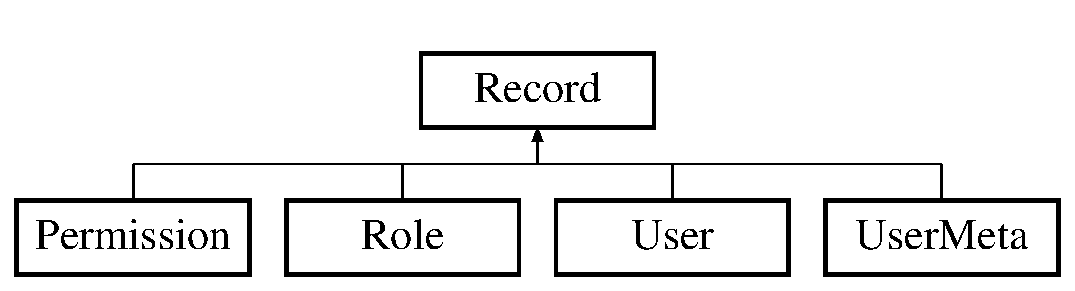
\includegraphics[height=2.000000cm]{class_record}
\end{center}
\end{figure}
\subsection*{Public Member Functions}
\begin{DoxyCompactItemize}
\item 
\hyperlink{class_record_a4e176c3a661053094339903c5cfc7942}{\-\_\-\-\_\-construct} (\$id=0)
\item 
\hyperlink{class_record_a7160b09d9d37ede69811a66dc9e4f272}{load} (\$id=0)
\item 
\hyperlink{class_record_afc8a3c62679cf00ade9f15fb2a6d6132}{save} ()
\item 
\hyperlink{class_record_a13bdffdd926f26b825ea57066334ff01}{delete} ()
\item 
\hyperlink{class_record_a93614c4fd6ba6715b5d339e6b4720d34}{form} (Array \$fields, \$legend='table\-\_\-name', \$submit=true)
\end{DoxyCompactItemize}
\subsection*{Data Fields}
\begin{DoxyCompactItemize}
\item 
\hyperlink{class_record_a19d2a3d21fe02053311fde465e6ae2e9}{\$columns}
\item 
\hyperlink{class_record_a9e6fc1ae0498be7d1e682f8bcc9299df}{\$meta}
\end{DoxyCompactItemize}
\subsection*{Protected Attributes}
\begin{DoxyCompactItemize}
\item 
\hyperlink{class_record_a1fa3127fc82f96b1436d871ef02be319}{\$db}
\item 
\hyperlink{class_record_ae8876a14058f368335baccf35af4a22b}{\$table}
\item 
\hyperlink{class_record_a927b0256b942a3ee89485f2649af7981}{\$primary\-Key} = 'id'
\end{DoxyCompactItemize}


\subsection{Constructor \& Destructor Documentation}
\hypertarget{class_record_a4e176c3a661053094339903c5cfc7942}{\index{Record@{Record}!\-\_\-\-\_\-construct@{\-\_\-\-\_\-construct}}
\index{\-\_\-\-\_\-construct@{\-\_\-\-\_\-construct}!Record@{Record}}
\subsubsection[{\-\_\-\-\_\-construct}]{\setlength{\rightskip}{0pt plus 5cm}\-\_\-\-\_\-construct (
\begin{DoxyParamCaption}
\item[{}]{\$id = {\ttfamily 0}}
\end{DoxyParamCaption}
)}}\label{class_record_a4e176c3a661053094339903c5cfc7942}
Initializes db and gets column information.


\begin{DoxyParams}[1]{Parameters}
string & {\em \$id} & The id to load automatically \\
\hline
\end{DoxyParams}


\subsection{Member Function Documentation}
\hypertarget{class_record_a13bdffdd926f26b825ea57066334ff01}{\index{Record@{Record}!delete@{delete}}
\index{delete@{delete}!Record@{Record}}
\subsubsection[{delete}]{\setlength{\rightskip}{0pt plus 5cm}delete (
\begin{DoxyParamCaption}
{}
\end{DoxyParamCaption}
)}}\label{class_record_a13bdffdd926f26b825ea57066334ff01}
Deletes this record from the database

\begin{DoxyReturn}{Returns}
bool True if delete is successful 
\end{DoxyReturn}
\hypertarget{class_record_a93614c4fd6ba6715b5d339e6b4720d34}{\index{Record@{Record}!form@{form}}
\index{form@{form}!Record@{Record}}
\subsubsection[{form}]{\setlength{\rightskip}{0pt plus 5cm}form (
\begin{DoxyParamCaption}
\item[{Array}]{\$fields, }
\item[{}]{\$legend = {\ttfamily 'table\-\_\-name'}, }
\item[{}]{\$submit = {\ttfamily true}}
\end{DoxyParamCaption}
)}}\label{class_record_a93614c4fd6ba6715b5d339e6b4720d34}
Shows an editable form


\begin{DoxyParams}[1]{Parameters}
Array & {\em \$fields} & An array of columns =$>$ labels \\
\hline
string & {\em \$legend} & Customize the fieldset legend \\
\hline
boolean & {\em \$submit} & Show the submit button? \\
\hline
\end{DoxyParams}
\begin{DoxyReturn}{Returns}
void returns nothing 
\end{DoxyReturn}
\hypertarget{class_record_a7160b09d9d37ede69811a66dc9e4f272}{\index{Record@{Record}!load@{load}}
\index{load@{load}!Record@{Record}}
\subsubsection[{load}]{\setlength{\rightskip}{0pt plus 5cm}load (
\begin{DoxyParamCaption}
\item[{}]{\$id = {\ttfamily 0}}
\end{DoxyParamCaption}
)}}\label{class_record_a7160b09d9d37ede69811a66dc9e4f272}
Loads a record as an object.


\begin{DoxyParams}[1]{Parameters}
integer & {\em \$id} & id of a record to load \\
\hline
\end{DoxyParams}
\begin{DoxyReturn}{Returns}
bool True if loaded correctly 
\end{DoxyReturn}
\hypertarget{class_record_afc8a3c62679cf00ade9f15fb2a6d6132}{\index{Record@{Record}!save@{save}}
\index{save@{save}!Record@{Record}}
\subsubsection[{save}]{\setlength{\rightskip}{0pt plus 5cm}save (
\begin{DoxyParamCaption}
{}
\end{DoxyParamCaption}
)}}\label{class_record_afc8a3c62679cf00ade9f15fb2a6d6132}
Saves the record to the database.

\begin{DoxyReturn}{Returns}
mixed Returns the Primary Key 
\end{DoxyReturn}


\subsection{Field Documentation}
\hypertarget{class_record_a19d2a3d21fe02053311fde465e6ae2e9}{\index{Record@{Record}!\$columns@{\$columns}}
\index{\$columns@{\$columns}!Record@{Record}}
\subsubsection[{\$columns}]{\setlength{\rightskip}{0pt plus 5cm}\$columns}}\label{class_record_a19d2a3d21fe02053311fde465e6ae2e9}
array The data of the record get loaded here \hypertarget{class_record_a1fa3127fc82f96b1436d871ef02be319}{\index{Record@{Record}!\$db@{\$db}}
\index{\$db@{\$db}!Record@{Record}}
\subsubsection[{\$db}]{\setlength{\rightskip}{0pt plus 5cm}\$db\hspace{0.3cm}{\ttfamily [protected]}}}\label{class_record_a1fa3127fc82f96b1436d871ef02be319}
P\-D\-O The P\-D\-O object \hypertarget{class_record_a9e6fc1ae0498be7d1e682f8bcc9299df}{\index{Record@{Record}!\$meta@{\$meta}}
\index{\$meta@{\$meta}!Record@{Record}}
\subsubsection[{\$meta}]{\setlength{\rightskip}{0pt plus 5cm}\$meta}}\label{class_record_a9e6fc1ae0498be7d1e682f8bcc9299df}
std\-Object The record meta data gets loaded here \hypertarget{class_record_a927b0256b942a3ee89485f2649af7981}{\index{Record@{Record}!\$primary\-Key@{\$primary\-Key}}
\index{\$primary\-Key@{\$primary\-Key}!Record@{Record}}
\subsubsection[{\$primary\-Key}]{\setlength{\rightskip}{0pt plus 5cm}\$primary\-Key = 'id'\hspace{0.3cm}{\ttfamily [protected]}}}\label{class_record_a927b0256b942a3ee89485f2649af7981}
string The primary key of the table \hypertarget{class_record_ae8876a14058f368335baccf35af4a22b}{\index{Record@{Record}!\$table@{\$table}}
\index{\$table@{\$table}!Record@{Record}}
\subsubsection[{\$table}]{\setlength{\rightskip}{0pt plus 5cm}\$table\hspace{0.3cm}{\ttfamily [protected]}}}\label{class_record_ae8876a14058f368335baccf35af4a22b}
string The name of the table 

The documentation for this class was generated from the following file\-:\begin{DoxyCompactItemize}
\item 
C\-:/\-Users/\-Jaime.\-Ushuaia/\-Documents/\-Git\-Hub/sleepy-\/mustache/modules/disabled/db/class.\-record.\-php\end{DoxyCompactItemize}

\hypertarget{class_request}{\section{Request Class Reference}
\label{class_request}\index{Request@{Request}}
}
Inheritance diagram for Request\-:\begin{figure}[H]
\begin{center}
\leavevmode
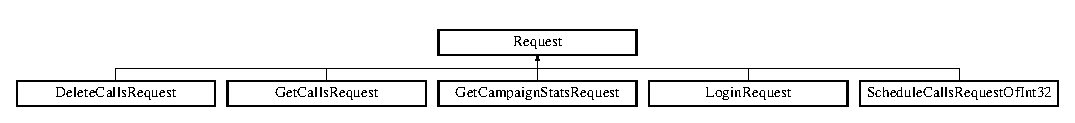
\includegraphics[height=1.204301cm]{class_request}
\end{center}
\end{figure}
\subsection*{Data Fields}
\begin{DoxyCompactItemize}
\item 
\hyperlink{class_request_af36f2c89cc01324e295786be80a30f3a}{\$\-Session\-Id}
\end{DoxyCompactItemize}


\subsection{Detailed Description}
The base \hyperlink{class_request}{Request} object 

\subsection{Field Documentation}
\hypertarget{class_request_af36f2c89cc01324e295786be80a30f3a}{\index{Request@{Request}!\$\-Session\-Id@{\$\-Session\-Id}}
\index{\$\-Session\-Id@{\$\-Session\-Id}!Request@{Request}}
\subsubsection[{\$\-Session\-Id}]{\setlength{\rightskip}{0pt plus 5cm}\$Session\-Id}}\label{class_request_af36f2c89cc01324e295786be80a30f3a}
String Session I\-D of the request 

The documentation for this class was generated from the following file\-:\begin{DoxyCompactItemize}
\item 
C\-:/\-Users/\-Jaime.\-Ushuaia/\-Documents/\-Git\-Hub/sleepy-\/mustache/modules/disabled/robotalker/class.\-robotalker.\-php\end{DoxyCompactItemize}

\hypertarget{class_robo_talker}{\section{Robo\-Talker Class Reference}
\label{class_robo_talker}\index{Robo\-Talker@{Robo\-Talker}}
}
\subsection*{Public Member Functions}
\begin{DoxyCompactItemize}
\item 
\hyperlink{class_robo_talker_a095c5d389db211932136b53f25f39685}{\-\_\-\-\_\-construct} ()
\item 
\hyperlink{class_robo_talker_acb6ab21469df29a582bee44e78f97edc}{Get\-Scheduled\-Calls} ()
\item 
\hyperlink{class_robo_talker_a7e73ba6712fb06fbcb1bbbc998ba5a0c}{Get\-Campaign\-Stats} (\$id)
\item 
\hyperlink{class_robo_talker_ac0650c287190d98e1d85ff9ef10a7404}{add} (\$phone\-Number)
\item 
\hyperlink{class_robo_talker_a6c473c02f29af893f4ad6983ead3ddb8}{delete} (\$phone\-Number)
\item 
\hyperlink{class_robo_talker_a96bef29f5a68282aac40e6b197e39d2b}{send\-Voicemail} ()
\end{DoxyCompactItemize}


\subsection{Detailed Description}
The \hyperlink{class_robo_talker}{Robo\-Talker} class controls the communication to the Web\-Service 

\subsection{Constructor \& Destructor Documentation}
\hypertarget{class_robo_talker_a095c5d389db211932136b53f25f39685}{\index{Robo\-Talker@{Robo\-Talker}!\-\_\-\-\_\-construct@{\-\_\-\-\_\-construct}}
\index{\-\_\-\-\_\-construct@{\-\_\-\-\_\-construct}!RoboTalker@{Robo\-Talker}}
\subsubsection[{\-\_\-\-\_\-construct}]{\setlength{\rightskip}{0pt plus 5cm}\-\_\-\-\_\-construct (
\begin{DoxyParamCaption}
{}
\end{DoxyParamCaption}
)}}\label{class_robo_talker_a095c5d389db211932136b53f25f39685}
Connects to webservice, login, store Session\-Id.

\begin{DoxyReturn}{Returns}
instance 
\end{DoxyReturn}


\subsection{Member Function Documentation}
\hypertarget{class_robo_talker_ac0650c287190d98e1d85ff9ef10a7404}{\index{Robo\-Talker@{Robo\-Talker}!add@{add}}
\index{add@{add}!RoboTalker@{Robo\-Talker}}
\subsubsection[{add}]{\setlength{\rightskip}{0pt plus 5cm}add (
\begin{DoxyParamCaption}
\item[{}]{\$phone\-Number}
\end{DoxyParamCaption}
)}}\label{class_robo_talker_ac0650c287190d98e1d85ff9ef10a7404}
Add a new Call. 
\begin{DoxyParams}[1]{Parameters}
int & {\em \$phone\-Number} & \mbox{[}description\mbox{]} \\
\hline
\end{DoxyParams}

\begin{DoxyExceptions}{Exceptions}
{\em Exception} & \\
\hline
\end{DoxyExceptions}
\begin{DoxyReturn}{Returns}
int Campaign\-Id 
\end{DoxyReturn}
\hypertarget{class_robo_talker_a6c473c02f29af893f4ad6983ead3ddb8}{\index{Robo\-Talker@{Robo\-Talker}!delete@{delete}}
\index{delete@{delete}!RoboTalker@{Robo\-Talker}}
\subsubsection[{delete}]{\setlength{\rightskip}{0pt plus 5cm}delete (
\begin{DoxyParamCaption}
\item[{}]{\$phone\-Number}
\end{DoxyParamCaption}
)}}\label{class_robo_talker_a6c473c02f29af893f4ad6983ead3ddb8}
Deletes a Call. 
\begin{DoxyParams}[1]{Parameters}
String & {\em \$phone\-Number} & A phone number to delete \\
\hline
\end{DoxyParams}

\begin{DoxyExceptions}{Exceptions}
{\em Exception} & If Delete fails \\
\hline
\end{DoxyExceptions}
\begin{DoxyReturn}{Returns}
array An Array of phone numbers deleted. 
\end{DoxyReturn}
\hypertarget{class_robo_talker_a7e73ba6712fb06fbcb1bbbc998ba5a0c}{\index{Robo\-Talker@{Robo\-Talker}!Get\-Campaign\-Stats@{Get\-Campaign\-Stats}}
\index{Get\-Campaign\-Stats@{Get\-Campaign\-Stats}!RoboTalker@{Robo\-Talker}}
\subsubsection[{Get\-Campaign\-Stats}]{\setlength{\rightskip}{0pt plus 5cm}Get\-Campaign\-Stats (
\begin{DoxyParamCaption}
\item[{}]{\$id}
\end{DoxyParamCaption}
)}}\label{class_robo_talker_a7e73ba6712fb06fbcb1bbbc998ba5a0c}
Gets all Campaign Stats


\begin{DoxyParams}{Parameters}
{\em \$id} & \\
\hline
\end{DoxyParams}
\begin{DoxyReturn}{Returns}
array Calls objects 
\end{DoxyReturn}
\hypertarget{class_robo_talker_acb6ab21469df29a582bee44e78f97edc}{\index{Robo\-Talker@{Robo\-Talker}!Get\-Scheduled\-Calls@{Get\-Scheduled\-Calls}}
\index{Get\-Scheduled\-Calls@{Get\-Scheduled\-Calls}!RoboTalker@{Robo\-Talker}}
\subsubsection[{Get\-Scheduled\-Calls}]{\setlength{\rightskip}{0pt plus 5cm}Get\-Scheduled\-Calls (
\begin{DoxyParamCaption}
{}
\end{DoxyParamCaption}
)}}\label{class_robo_talker_acb6ab21469df29a582bee44e78f97edc}
Gets all scheduled calls

\begin{DoxyReturn}{Returns}
array Calls objects 
\end{DoxyReturn}
\hypertarget{class_robo_talker_a96bef29f5a68282aac40e6b197e39d2b}{\index{Robo\-Talker@{Robo\-Talker}!send\-Voicemail@{send\-Voicemail}}
\index{send\-Voicemail@{send\-Voicemail}!RoboTalker@{Robo\-Talker}}
\subsubsection[{send\-Voicemail}]{\setlength{\rightskip}{0pt plus 5cm}send\-Voicemail (
\begin{DoxyParamCaption}
{}
\end{DoxyParamCaption}
)}}\label{class_robo_talker_a96bef29f5a68282aac40e6b197e39d2b}
Toggle a voicemail. \begin{DoxyReturn}{Returns}
nothing 
\end{DoxyReturn}


The documentation for this class was generated from the following file\-:\begin{DoxyCompactItemize}
\item 
C\-:/\-Users/\-Jaime.\-Ushuaia/\-Documents/\-Git\-Hub/sleepy-\/mustache/modules/disabled/robotalker/class.\-robotalker.\-php\end{DoxyCompactItemize}

\hypertarget{class_role}{\section{Role Class Reference}
\label{class_role}\index{Role@{Role}}
}
Inheritance diagram for Role\-:\begin{figure}[H]
\begin{center}
\leavevmode
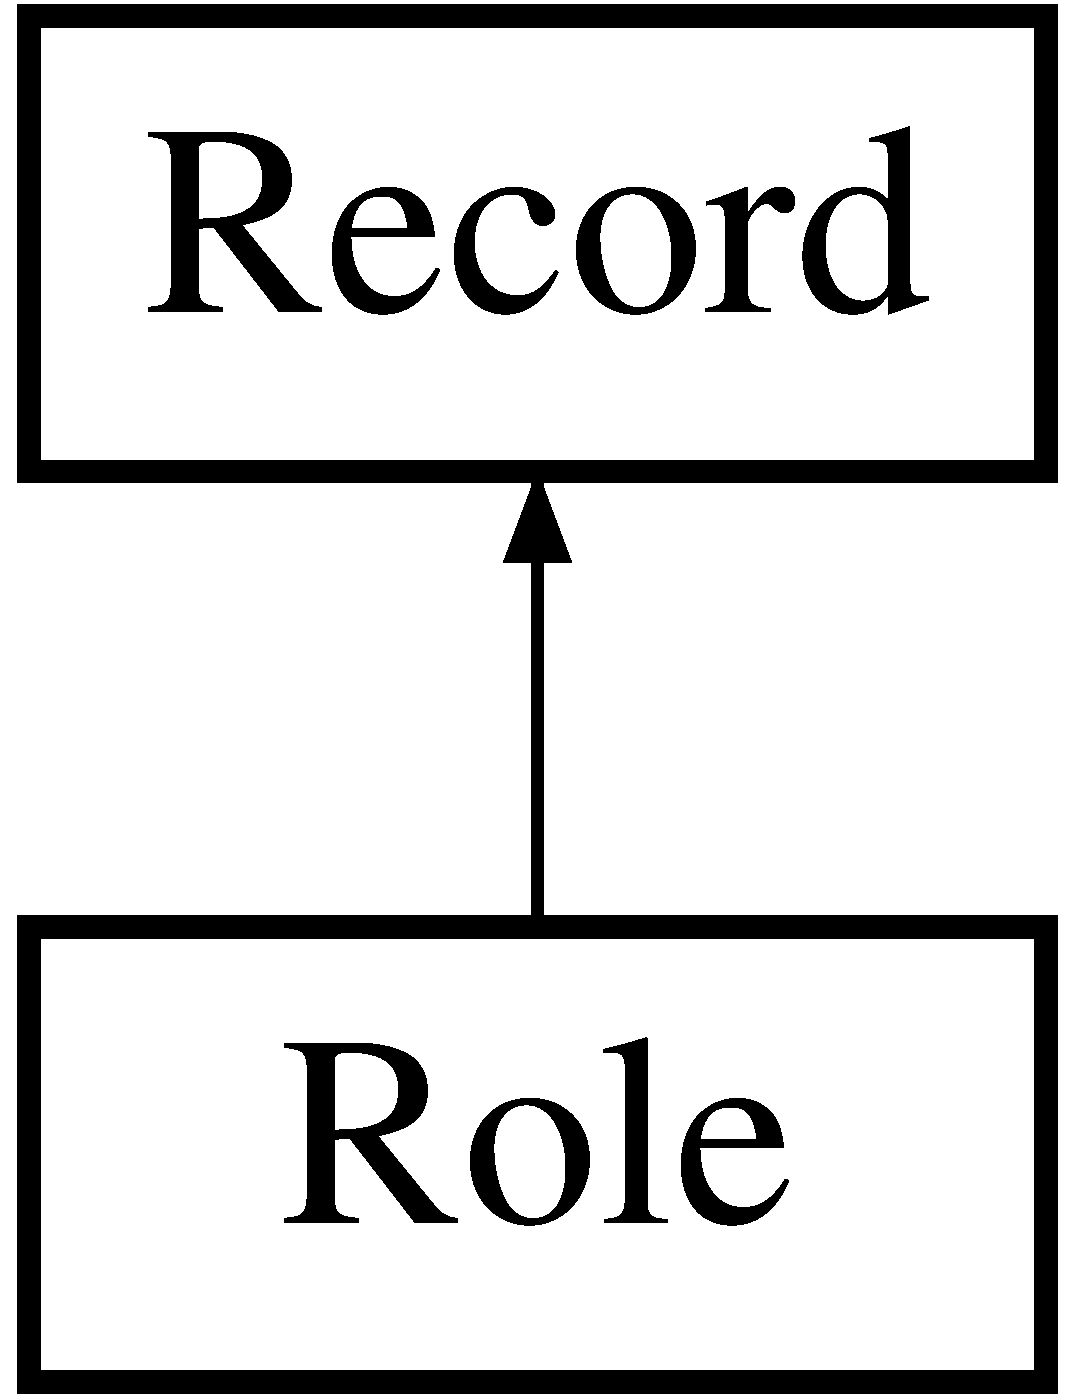
\includegraphics[height=2.000000cm]{class_role}
\end{center}
\end{figure}
\subsection*{Public Member Functions}
\begin{DoxyCompactItemize}
\item 
\hyperlink{class_role_a610dd05d53d99e1ddc05596468eb4914}{get\-Permission} (\$key)
\item 
\hyperlink{class_role_a7160b09d9d37ede69811a66dc9e4f272}{load} (\$id=0)
\item 
\hyperlink{class_role_a20b0e06124acf9f1e66afa1b1c8f996a}{set\-Permission} (\$key, \$value)
\end{DoxyCompactItemize}
\subsection*{Data Fields}
\begin{DoxyCompactItemize}
\item 
\hyperlink{class_role_ae8876a14058f368335baccf35af4a22b}{\$table} = 'roles'
\end{DoxyCompactItemize}
\subsection*{Additional Inherited Members}


\subsection{Detailed Description}


Definition at line 155 of file class.\-user.\-php.



\subsection{Member Function Documentation}
\hypertarget{class_role_a610dd05d53d99e1ddc05596468eb4914}{\index{Role@{Role}!get\-Permission@{get\-Permission}}
\index{get\-Permission@{get\-Permission}!Role@{Role}}
\subsubsection[{get\-Permission}]{\setlength{\rightskip}{0pt plus 5cm}get\-Permission (
\begin{DoxyParamCaption}
\item[{}]{\$key}
\end{DoxyParamCaption}
)}}\label{class_role_a610dd05d53d99e1ddc05596468eb4914}


Definition at line 159 of file class.\-user.\-php.


\begin{DoxyCode}
                                                                  \{
                                             \textcolor{keywordflow}{if} (isset($this->\_permissions[$key
      ])) \{
                                                            \textcolor{keywordflow}{return} $this->
      \_permissions[$key];
                                             \} \textcolor{keywordflow}{else} \{
                                                            \textcolor{keywordflow}{throw} \textcolor{keyword}{new} Exception
      (\textcolor{stringliteral}{"\{$key\} permission does not exist."});
                                             \}
                              \}
\end{DoxyCode}
\hypertarget{class_role_a7160b09d9d37ede69811a66dc9e4f272}{\index{Role@{Role}!load@{load}}
\index{load@{load}!Role@{Role}}
\subsubsection[{load}]{\setlength{\rightskip}{0pt plus 5cm}load (
\begin{DoxyParamCaption}
\item[{}]{\$id = {\ttfamily 0}}
\end{DoxyParamCaption}
)}}\label{class_role_a7160b09d9d37ede69811a66dc9e4f272}


Definition at line 167 of file class.\-user.\-php.


\begin{DoxyCode}
                                                          \{
                                             parent::load($id);

                                             \textcolor{comment}{// Load permissions}
                                             $query = $this->db->query(\textcolor{stringliteral}{"SELECT
       * FROM permissions where role\_id=\{$this->columns['id']\}"});
                                             $query->setFetchMode(
      PDO::FETCH\_ASSOC);
                                             $query->execute();

                                             $permissions = $query->fetchAll();

                                             \textcolor{keywordflow}{foreach} ($permissions as $p) \{
                                                            $temp = \textcolor{keyword}{new} 
      \hyperlink{class_permission}{Permission}($p[\textcolor{stringliteral}{'id'}]);
                                                            $this->\_permissions
      [$temp->columns[\textcolor{stringliteral}{'key'}]] = $temp->columns[\textcolor{stringliteral}{'value'}];
                                             \}
                              \}
\end{DoxyCode}
\hypertarget{class_role_a20b0e06124acf9f1e66afa1b1c8f996a}{\index{Role@{Role}!set\-Permission@{set\-Permission}}
\index{set\-Permission@{set\-Permission}!Role@{Role}}
\subsubsection[{set\-Permission}]{\setlength{\rightskip}{0pt plus 5cm}set\-Permission (
\begin{DoxyParamCaption}
\item[{}]{\$key, }
\item[{}]{\$value}
\end{DoxyParamCaption}
)}}\label{class_role_a20b0e06124acf9f1e66afa1b1c8f996a}


Definition at line 183 of file class.\-user.\-php.


\begin{DoxyCode}
                                                                          \{
                                             \textcolor{keywordflow}{if} (isset($this->\_permissions[$key
      ])) \{
                                                            $this->\_permissions
      [$key] = $value;
                                             \} \textcolor{keywordflow}{else} \{
                                                            $temp = \textcolor{keyword}{new} 
      \hyperlink{class_permission}{Permission}();
                                                            $temp->columns[\textcolor{stringliteral}{'key
      '}] = $key;
                                                            $temp->columns[\textcolor{stringliteral}{'
      value'}] = $value;
                                                            $temp->save();
                                             \}
                              \}
\end{DoxyCode}


\subsection{Field Documentation}
\hypertarget{class_role_ae8876a14058f368335baccf35af4a22b}{\index{Role@{Role}!\$table@{\$table}}
\index{\$table@{\$table}!Role@{Role}}
\subsubsection[{\$table}]{\setlength{\rightskip}{0pt plus 5cm}\$table = 'roles'}}\label{class_role_ae8876a14058f368335baccf35af4a22b}


Definition at line 156 of file class.\-user.\-php.



The documentation for this class was generated from the following file\-:\begin{DoxyCompactItemize}
\item 
modules/disabled/users/\hyperlink{class_8user_8php}{class.\-user.\-php}\end{DoxyCompactItemize}

\hypertarget{class_schedule_calls_request_of_int32}{\section{Schedule\-Calls\-Request\-Of\-Int32 Class Reference}
\label{class_schedule_calls_request_of_int32}\index{Schedule\-Calls\-Request\-Of\-Int32@{Schedule\-Calls\-Request\-Of\-Int32}}
}
Inheritance diagram for Schedule\-Calls\-Request\-Of\-Int32\-:\begin{figure}[H]
\begin{center}
\leavevmode
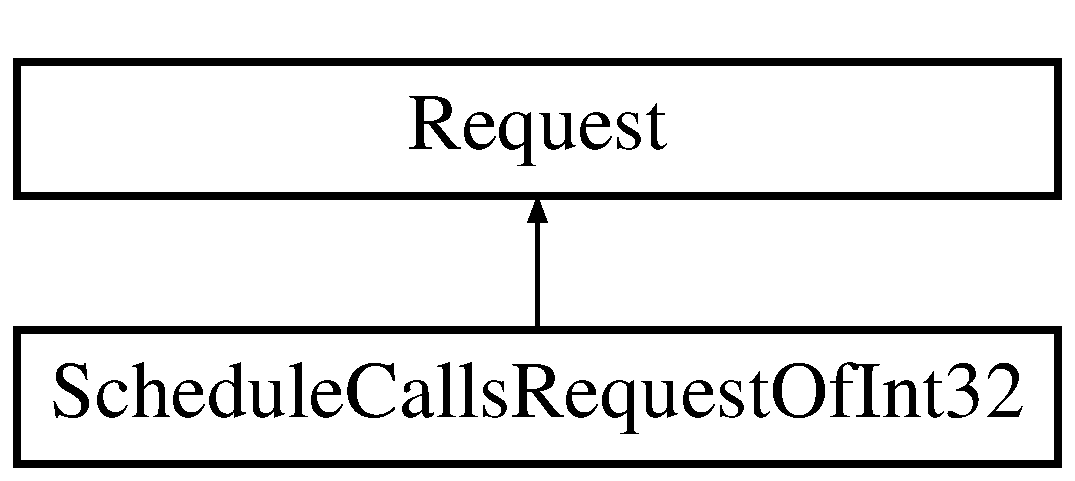
\includegraphics[height=2.000000cm]{class_schedule_calls_request_of_int32}
\end{center}
\end{figure}
\subsection*{Data Fields}
\begin{DoxyCompactItemize}
\item 
\hyperlink{class_schedule_calls_request_of_int32_a33ad804cbe51afe501872f4363f0c068}{\$\-Recipients}
\item 
\hyperlink{class_schedule_calls_request_of_int32_ab23576849f64a6b190167099cfab7eae}{\$\-Message}
\item 
\hyperlink{class_schedule_calls_request_of_int32_ab8946a1492b48b7d64a4e6f298903f74}{\$\-Voice\-Mail\-Message}
\item 
\hyperlink{class_schedule_calls_request_of_int32_ad8484f456a9bd6b83b5f077db37b7558}{\$\-Schedule\-Type}
\item 
\hyperlink{class_schedule_calls_request_of_int32_a2f8fa05008bd8e80ae9cb79699e0ed2c}{\$\-Start\-Time}
\item 
\hyperlink{class_schedule_calls_request_of_int32_ab7205c64d4caf57ad5c439d161116d8e}{\$\-End\-Time}
\item 
\hyperlink{class_schedule_calls_request_of_int32_a541b96a58d5cadab10a165a562fc066e}{\$\-Days}
\item 
\hyperlink{class_schedule_calls_request_of_int32_a06a0c2a526e2a41abe73b0ffdf2932ee}{\$\-Interval}
\item 
\hyperlink{class_schedule_calls_request_of_int32_a7c6546640ba3eafd143d8f0e6805de27}{\$\-Priority}
\item 
\hyperlink{class_schedule_calls_request_of_int32_afcd9214c7e03e9e066611fb7ee041fb9}{\$\-Confirmation}
\end{DoxyCompactItemize}


\subsection{Detailed Description}
The object sent for the Schedule\-Calls method 

\subsection{Field Documentation}
\hypertarget{class_schedule_calls_request_of_int32_afcd9214c7e03e9e066611fb7ee041fb9}{\index{Schedule\-Calls\-Request\-Of\-Int32@{Schedule\-Calls\-Request\-Of\-Int32}!\$\-Confirmation@{\$\-Confirmation}}
\index{\$\-Confirmation@{\$\-Confirmation}!ScheduleCallsRequestOfInt32@{Schedule\-Calls\-Request\-Of\-Int32}}
\subsubsection[{\$\-Confirmation}]{\setlength{\rightskip}{0pt plus 5cm}\$Confirmation}}\label{class_schedule_calls_request_of_int32_afcd9214c7e03e9e066611fb7ee041fb9}
Bool Do you want a confirmation email? \hypertarget{class_schedule_calls_request_of_int32_a541b96a58d5cadab10a165a562fc066e}{\index{Schedule\-Calls\-Request\-Of\-Int32@{Schedule\-Calls\-Request\-Of\-Int32}!\$\-Days@{\$\-Days}}
\index{\$\-Days@{\$\-Days}!ScheduleCallsRequestOfInt32@{Schedule\-Calls\-Request\-Of\-Int32}}
\subsubsection[{\$\-Days}]{\setlength{\rightskip}{0pt plus 5cm}\$Days}}\label{class_schedule_calls_request_of_int32_a541b96a58d5cadab10a165a562fc066e}
Week\-Days The Days of the week to run schedule \hypertarget{class_schedule_calls_request_of_int32_ab7205c64d4caf57ad5c439d161116d8e}{\index{Schedule\-Calls\-Request\-Of\-Int32@{Schedule\-Calls\-Request\-Of\-Int32}!\$\-End\-Time@{\$\-End\-Time}}
\index{\$\-End\-Time@{\$\-End\-Time}!ScheduleCallsRequestOfInt32@{Schedule\-Calls\-Request\-Of\-Int32}}
\subsubsection[{\$\-End\-Time}]{\setlength{\rightskip}{0pt plus 5cm}\$End\-Time}}\label{class_schedule_calls_request_of_int32_ab7205c64d4caf57ad5c439d161116d8e}
Date\-Time The End time \hypertarget{class_schedule_calls_request_of_int32_a06a0c2a526e2a41abe73b0ffdf2932ee}{\index{Schedule\-Calls\-Request\-Of\-Int32@{Schedule\-Calls\-Request\-Of\-Int32}!\$\-Interval@{\$\-Interval}}
\index{\$\-Interval@{\$\-Interval}!ScheduleCallsRequestOfInt32@{Schedule\-Calls\-Request\-Of\-Int32}}
\subsubsection[{\$\-Interval}]{\setlength{\rightskip}{0pt plus 5cm}\$Interval}}\label{class_schedule_calls_request_of_int32_a06a0c2a526e2a41abe73b0ffdf2932ee}
Int How ofter to run the schedule \hypertarget{class_schedule_calls_request_of_int32_ab23576849f64a6b190167099cfab7eae}{\index{Schedule\-Calls\-Request\-Of\-Int32@{Schedule\-Calls\-Request\-Of\-Int32}!\$\-Message@{\$\-Message}}
\index{\$\-Message@{\$\-Message}!ScheduleCallsRequestOfInt32@{Schedule\-Calls\-Request\-Of\-Int32}}
\subsubsection[{\$\-Message}]{\setlength{\rightskip}{0pt plus 5cm}\$Message}}\label{class_schedule_calls_request_of_int32_ab23576849f64a6b190167099cfab7eae}
String Optional. String Optional. \hypertarget{class_schedule_calls_request_of_int32_a7c6546640ba3eafd143d8f0e6805de27}{\index{Schedule\-Calls\-Request\-Of\-Int32@{Schedule\-Calls\-Request\-Of\-Int32}!\$\-Priority@{\$\-Priority}}
\index{\$\-Priority@{\$\-Priority}!ScheduleCallsRequestOfInt32@{Schedule\-Calls\-Request\-Of\-Int32}}
\subsubsection[{\$\-Priority}]{\setlength{\rightskip}{0pt plus 5cm}\$Priority}}\label{class_schedule_calls_request_of_int32_a7c6546640ba3eafd143d8f0e6805de27}
Int Schedule priority \hypertarget{class_schedule_calls_request_of_int32_a33ad804cbe51afe501872f4363f0c068}{\index{Schedule\-Calls\-Request\-Of\-Int32@{Schedule\-Calls\-Request\-Of\-Int32}!\$\-Recipients@{\$\-Recipients}}
\index{\$\-Recipients@{\$\-Recipients}!ScheduleCallsRequestOfInt32@{Schedule\-Calls\-Request\-Of\-Int32}}
\subsubsection[{\$\-Recipients}]{\setlength{\rightskip}{0pt plus 5cm}\$Recipients}}\label{class_schedule_calls_request_of_int32_a33ad804cbe51afe501872f4363f0c068}
Message\-Recipient$<$int32$>$ Mandatory. \hypertarget{class_schedule_calls_request_of_int32_ad8484f456a9bd6b83b5f077db37b7558}{\index{Schedule\-Calls\-Request\-Of\-Int32@{Schedule\-Calls\-Request\-Of\-Int32}!\$\-Schedule\-Type@{\$\-Schedule\-Type}}
\index{\$\-Schedule\-Type@{\$\-Schedule\-Type}!ScheduleCallsRequestOfInt32@{Schedule\-Calls\-Request\-Of\-Int32}}
\subsubsection[{\$\-Schedule\-Type}]{\setlength{\rightskip}{0pt plus 5cm}\$Schedule\-Type}}\label{class_schedule_calls_request_of_int32_ad8484f456a9bd6b83b5f077db37b7558}
Campaign\-Types Optional. \hypertarget{class_schedule_calls_request_of_int32_a2f8fa05008bd8e80ae9cb79699e0ed2c}{\index{Schedule\-Calls\-Request\-Of\-Int32@{Schedule\-Calls\-Request\-Of\-Int32}!\$\-Start\-Time@{\$\-Start\-Time}}
\index{\$\-Start\-Time@{\$\-Start\-Time}!ScheduleCallsRequestOfInt32@{Schedule\-Calls\-Request\-Of\-Int32}}
\subsubsection[{\$\-Start\-Time}]{\setlength{\rightskip}{0pt plus 5cm}\$Start\-Time}}\label{class_schedule_calls_request_of_int32_a2f8fa05008bd8e80ae9cb79699e0ed2c}
Date\-Time The Start Time \hypertarget{class_schedule_calls_request_of_int32_ab8946a1492b48b7d64a4e6f298903f74}{\index{Schedule\-Calls\-Request\-Of\-Int32@{Schedule\-Calls\-Request\-Of\-Int32}!\$\-Voice\-Mail\-Message@{\$\-Voice\-Mail\-Message}}
\index{\$\-Voice\-Mail\-Message@{\$\-Voice\-Mail\-Message}!ScheduleCallsRequestOfInt32@{Schedule\-Calls\-Request\-Of\-Int32}}
\subsubsection[{\$\-Voice\-Mail\-Message}]{\setlength{\rightskip}{0pt plus 5cm}\$Voice\-Mail\-Message}}\label{class_schedule_calls_request_of_int32_ab8946a1492b48b7d64a4e6f298903f74}
Int Voicemail Message I\-D 

The documentation for this class was generated from the following file\-:\begin{DoxyCompactItemize}
\item 
C\-:/\-Users/\-Jaime.\-Ushuaia/\-Documents/\-Git\-Hub/sleepy-\/mustache/include/class.\-robotalker.\-php\end{DoxyCompactItemize}

\hypertarget{class_template}{\section{Template Class Reference}
\label{class_template}\index{Template@{Template}}
}
\subsection*{Public Member Functions}
\begin{DoxyCompactItemize}
\item 
\hyperlink{class_template_a6ebd85d8c80be61c2f20f0bfeb9b5f7b}{set\-Template} (\$file)
\item 
\hyperlink{class_template_a5efa1ad8f3267178937b8fb23003bbd4}{\-\_\-\-\_\-construct} (\$template='')
\item 
\hyperlink{class_template_a820993178e7ede5e791288b36b9cef57}{bind} (\$placeholder, \$value)
\item 
\hyperlink{class_template_a309bb1dc9b92dd7ad5348e48245468f8}{bind\-Start} ()
\item 
\hyperlink{class_template_a71662e1be36ebe0eeabd5fa629e5c538}{bind\-Stop} (\$placeholder)
\item 
\hyperlink{class_template_a24a9bf83a1002d46ece83a93d14bd921}{get} (\$key)
\item 
\hyperlink{class_template_a2b8e3779f5bd8c38f70307574859bd36}{show} ()
\end{DoxyCompactItemize}
\subsection*{Data Fields}
\begin{DoxyCompactItemize}
\item 
\hyperlink{class_template_aed02cd2cd0ee08bd99a2ac1ef4f955ce}{\$extension} = \char`\"{}.tpl\char`\"{}
\item 
\hyperlink{class_template_a1b07c630eb02f770a082a013373a16d6}{\$directory}
\end{DoxyCompactItemize}
\subsection*{Protected Attributes}
\begin{DoxyCompactItemize}
\item 
\hyperlink{class_template_abddaf0b77086e2b7d920f5d1a9616889}{\$\-\_\-file}
\item 
\hyperlink{class_template_a5a3006290f2de94fff2dd63ca739d15a}{\$\-\_\-data} = array()
\end{DoxyCompactItemize}


\subsection{Detailed Description}


Definition at line 45 of file class.\-template.\-php.



\subsection{Constructor \& Destructor Documentation}
\hypertarget{class_template_a5efa1ad8f3267178937b8fb23003bbd4}{\index{Template@{Template}!\-\_\-\-\_\-construct@{\-\_\-\-\_\-construct}}
\index{\-\_\-\-\_\-construct@{\-\_\-\-\_\-construct}!Template@{Template}}
\subsubsection[{\-\_\-\-\_\-construct}]{\setlength{\rightskip}{0pt plus 5cm}\-\_\-\-\_\-construct (
\begin{DoxyParamCaption}
\item[{}]{\$template = {\ttfamily ''}}
\end{DoxyParamCaption}
)}}\label{class_template_a5efa1ad8f3267178937b8fb23003bbd4}
The constructor 
\begin{DoxyParams}[1]{Parameters}
string & {\em \$template} & The name of the template \\
\hline
\end{DoxyParams}


Definition at line 207 of file class.\-template.\-php.


\begin{DoxyCode}
                                                         \{
                              \hyperlink{class_hook_afff7a7869d2dd304043b69a3fff24655}{Hook::addAction}(\textcolor{stringliteral}{'template\_start'});
                              $this->directory = \hyperlink{global_8php_a504552fd43e46a0032aa3f2895349f22}{DIRBASE} . \textcolor{stringliteral}{"/templates/"}
      ;
                              
                              \textcolor{keywordflow}{if} (!empty($template)) \{
                                             $this->\hyperlink{class_template_a6ebd85d8c80be61c2f20f0bfeb9b5f7b}{setTemplate}(
      $template);
                              \}
               \}
\end{DoxyCode}


\subsection{Member Function Documentation}
\hypertarget{class_template_a820993178e7ede5e791288b36b9cef57}{\index{Template@{Template}!bind@{bind}}
\index{bind@{bind}!Template@{Template}}
\subsubsection[{bind}]{\setlength{\rightskip}{0pt plus 5cm}bind (
\begin{DoxyParamCaption}
\item[{}]{\$placeholder, }
\item[{}]{\$value}
\end{DoxyParamCaption}
)}}\label{class_template_a820993178e7ede5e791288b36b9cef57}
Binds data to the template placeholders 
\begin{DoxyParams}[1]{Parameters}
string & {\em \$placeholder} & The template placeholder \\
\hline
mixed & {\em \$value} & The value that replaced the placeholder \\
\hline
\end{DoxyParams}


Definition at line 221 of file class.\-template.\-php.


\begin{DoxyCode}
                                                          \{
                              $this->\_data[trim(strtolower($placeholder))] = 
      $value; 
               \}
\end{DoxyCode}
\hypertarget{class_template_a309bb1dc9b92dd7ad5348e48245468f8}{\index{Template@{Template}!bind\-Start@{bind\-Start}}
\index{bind\-Start@{bind\-Start}!Template@{Template}}
\subsubsection[{bind\-Start}]{\setlength{\rightskip}{0pt plus 5cm}bind\-Start (
\begin{DoxyParamCaption}
{}
\end{DoxyParamCaption}
)}}\label{class_template_a309bb1dc9b92dd7ad5348e48245468f8}
Starts a buffer that will bind data to the template placeholders. The buffer will capture anything you output until \$this-\/$>$\hyperlink{class_template_a71662e1be36ebe0eeabd5fa629e5c538}{bind\-Stop()} 

Definition at line 229 of file class.\-template.\-php.


\begin{DoxyCode}
                                           \{
                              ob\_start();
               \}
\end{DoxyCode}
\hypertarget{class_template_a71662e1be36ebe0eeabd5fa629e5c538}{\index{Template@{Template}!bind\-Stop@{bind\-Stop}}
\index{bind\-Stop@{bind\-Stop}!Template@{Template}}
\subsubsection[{bind\-Stop}]{\setlength{\rightskip}{0pt plus 5cm}bind\-Stop (
\begin{DoxyParamCaption}
\item[{}]{\$placeholder}
\end{DoxyParamCaption}
)}}\label{class_template_a71662e1be36ebe0eeabd5fa629e5c538}
Stops the buffer that binds data to the template placeholders 
\begin{DoxyParams}[1]{Parameters}
string & {\em \$placeholder} & The template placeholder \\
\hline
\end{DoxyParams}


Definition at line 237 of file class.\-template.\-php.


\begin{DoxyCode}
                                                      \{
                              $content = ob\_get\_contents();
                              ob\_end\_clean();
                              $this->\_data[trim(strtolower($placeholder))] = 
      $content;
               \}
\end{DoxyCode}
\hypertarget{class_template_a24a9bf83a1002d46ece83a93d14bd921}{\index{Template@{Template}!get@{get}}
\index{get@{get}!Template@{Template}}
\subsubsection[{get}]{\setlength{\rightskip}{0pt plus 5cm}get (
\begin{DoxyParamCaption}
\item[{}]{\$key}
\end{DoxyParamCaption}
)}}\label{class_template_a24a9bf83a1002d46ece83a93d14bd921}
Gets the data for a placeholder 
\begin{DoxyParams}[1]{Parameters}
string & {\em \$placeholder} & The placeholder \\
\hline
\end{DoxyParams}
\begin{DoxyReturn}{Returns}
mixed The data stored in the placeholder 
\end{DoxyReturn}


Definition at line 248 of file class.\-template.\-php.


\begin{DoxyCode}
                                         \{
                              \textcolor{keywordflow}{return} \hyperlink{class_hook_a6489ed6b12329279b9e7cae26afc4dd6}{Hook::addFilter}(\textcolor{stringliteral}{'
      template\_get\_'} . $key, $this->\_data[$key]);
               \}
\end{DoxyCode}
\hypertarget{class_template_a6ebd85d8c80be61c2f20f0bfeb9b5f7b}{\index{Template@{Template}!set\-Template@{set\-Template}}
\index{set\-Template@{set\-Template}!Template@{Template}}
\subsubsection[{set\-Template}]{\setlength{\rightskip}{0pt plus 5cm}set\-Template (
\begin{DoxyParamCaption}
\item[{}]{\$file}
\end{DoxyParamCaption}
)}}\label{class_template_a6ebd85d8c80be61c2f20f0bfeb9b5f7b}
Sets the template to use. 
\begin{DoxyParams}{Parameters}
{\em \mbox{[}type\mbox{]}} & \$file \mbox{[}description\mbox{]} \\
\hline
\end{DoxyParams}


Definition at line 103 of file class.\-template.\-php.


\begin{DoxyCode}
                                                  \{
                              $this->\_file = $file;
               \}
\end{DoxyCode}
\hypertarget{class_template_a2b8e3779f5bd8c38f70307574859bd36}{\index{Template@{Template}!show@{show}}
\index{show@{show}!Template@{Template}}
\subsubsection[{show}]{\setlength{\rightskip}{0pt plus 5cm}show (
\begin{DoxyParamCaption}
{}
\end{DoxyParamCaption}
)}}\label{class_template_a2b8e3779f5bd8c38f70307574859bd36}
Shows the rendered template 

Definition at line 255 of file class.\-template.\-php.


\begin{DoxyCode}
                                      \{
                              \textcolor{comment}{// Check if template is ok}
                              $this->checkTemplate($this->\_file);

                              \textcolor{comment}{// Render template file}
                              ob\_start();
                              include($this->directory . $this->\_file . $this->
      extension);
                              $template = $this->render(ob\_get\_contents(), 
      $this->\_data) ;
                              ob\_end\_clean();

                              $template = \hyperlink{class_hook_a6489ed6b12329279b9e7cae26afc4dd6}{Hook::addFilter}(\textcolor{stringliteral}{'
      render\_template\_'} . $this->\_file, $template);
                              echo \hyperlink{class_hook_a6489ed6b12329279b9e7cae26afc4dd6}{Hook::addFilter}(\textcolor{stringliteral}{'
      render\_template'}, $template);
               \}
\end{DoxyCode}


\subsection{Field Documentation}
\hypertarget{class_template_a5a3006290f2de94fff2dd63ca739d15a}{\index{Template@{Template}!\$\-\_\-data@{\$\-\_\-data}}
\index{\$\-\_\-data@{\$\-\_\-data}!Template@{Template}}
\subsubsection[{\$\-\_\-data}]{\setlength{\rightskip}{0pt plus 5cm}\$\-\_\-data = array()\hspace{0.3cm}{\ttfamily [protected]}}}\label{class_template_a5a3006290f2de94fff2dd63ca739d15a}
array The data bound to the template 

Definition at line 66 of file class.\-template.\-php.

\hypertarget{class_template_abddaf0b77086e2b7d920f5d1a9616889}{\index{Template@{Template}!\$\-\_\-file@{\$\-\_\-file}}
\index{\$\-\_\-file@{\$\-\_\-file}!Template@{Template}}
\subsubsection[{\$\-\_\-file}]{\setlength{\rightskip}{0pt plus 5cm}\$\-\_\-file\hspace{0.3cm}{\ttfamily [protected]}}}\label{class_template_abddaf0b77086e2b7d920f5d1a9616889}
string The template file 

Definition at line 60 of file class.\-template.\-php.

\hypertarget{class_template_a1b07c630eb02f770a082a013373a16d6}{\index{Template@{Template}!\$directory@{\$directory}}
\index{\$directory@{\$directory}!Template@{Template}}
\subsubsection[{\$directory}]{\setlength{\rightskip}{0pt plus 5cm}\$directory}}\label{class_template_a1b07c630eb02f770a082a013373a16d6}
string The template directory 

Definition at line 54 of file class.\-template.\-php.

\hypertarget{class_template_aed02cd2cd0ee08bd99a2ac1ef4f955ce}{\index{Template@{Template}!\$extension@{\$extension}}
\index{\$extension@{\$extension}!Template@{Template}}
\subsubsection[{\$extension}]{\setlength{\rightskip}{0pt plus 5cm}\$extension = \char`\"{}.tpl\char`\"{}}}\label{class_template_aed02cd2cd0ee08bd99a2ac1ef4f955ce}
string The extension for template files 

Definition at line 49 of file class.\-template.\-php.



The documentation for this class was generated from the following file\-:\begin{DoxyCompactItemize}
\item 
include/\hyperlink{class_8template_8php}{class.\-template.\-php}\end{DoxyCompactItemize}

\hypertarget{class_user}{\section{User Class Reference}
\label{class_user}\index{User@{User}}
}
Inheritance diagram for User\-:\begin{figure}[H]
\begin{center}
\leavevmode
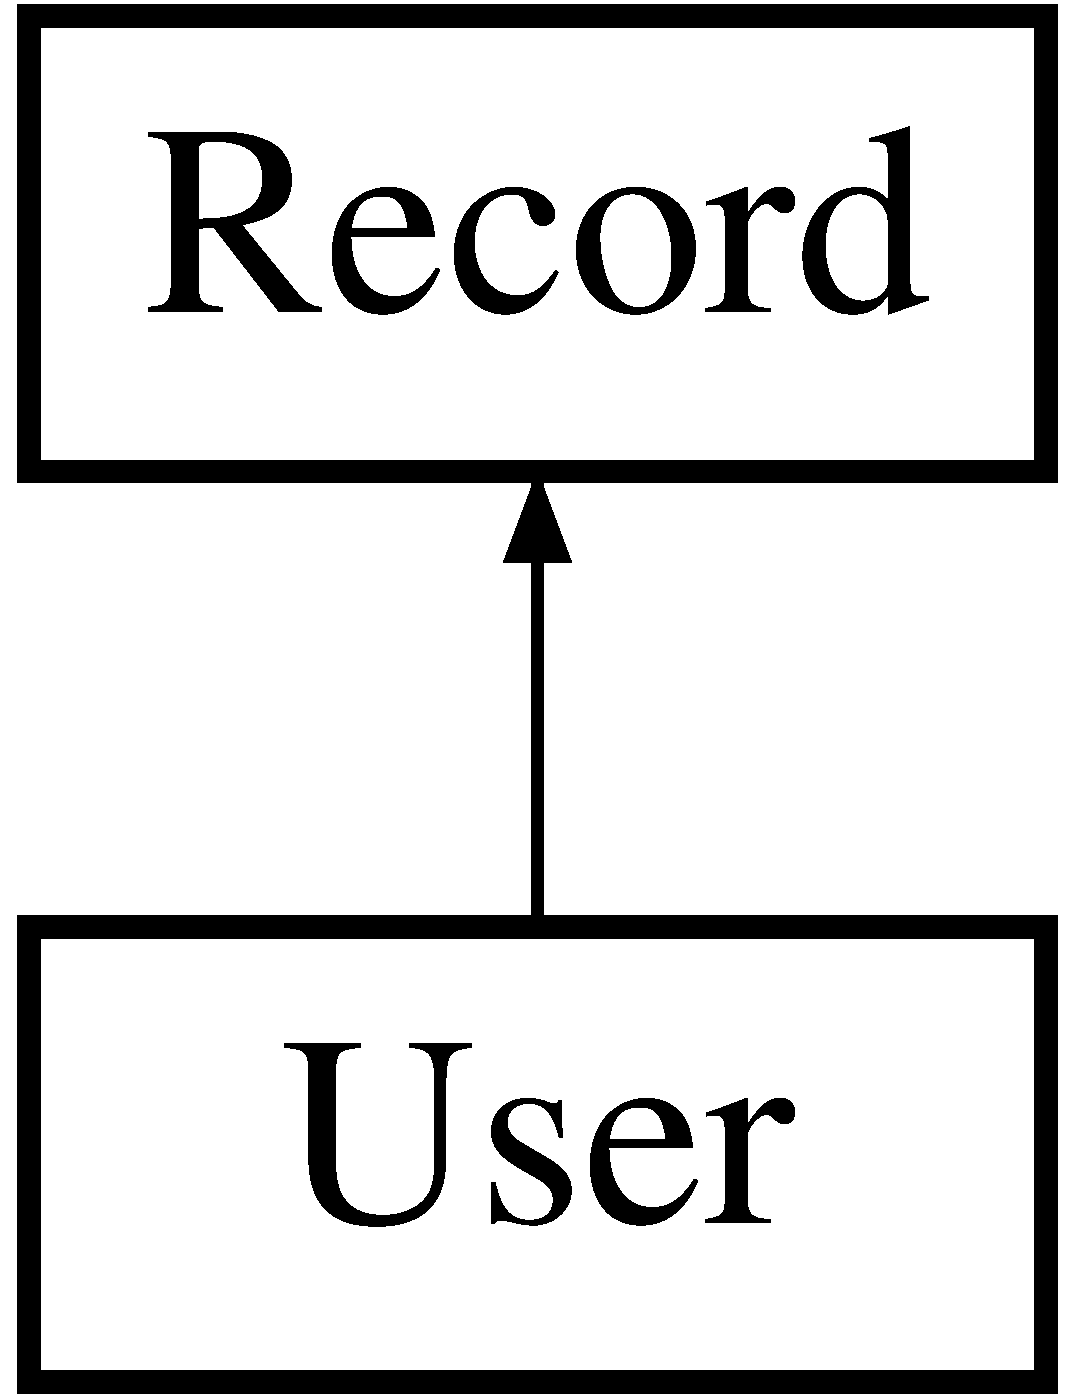
\includegraphics[height=2.000000cm]{class_user}
\end{center}
\end{figure}
\subsection*{Public Member Functions}
\begin{DoxyCompactItemize}
\item 
\hyperlink{class_user_a1e96415be573b36d4160d6ed1f6f40d3}{authenticate} (\$email, \$pass)
\item 
\hyperlink{class_user_a610dd05d53d99e1ddc05596468eb4914}{get\-Permission} (\$key)
\item 
\hyperlink{class_user_ab62d4b3c3a14ab592768235dad6deb63}{get\-User\-Data} (\$key)
\item 
\hyperlink{class_user_a7160b09d9d37ede69811a66dc9e4f272}{load} (\$id=0)
\item 
\hyperlink{class_user_a96f600de7f4fe416bf8565d9d0eebee4}{set\-User\-Data} (\$key, \$value)
\item 
\hyperlink{class_user_a8cdc6b049e470fac0e97101e4f353a05}{salt\-Password} (\$pass)
\item 
\hyperlink{class_user_afc8a3c62679cf00ade9f15fb2a6d6132}{save} ()
\item 
\hyperlink{class_user_a2f27c20674620565aa8b3433bffe305d}{is\-Loaded} ()
\item 
\hyperlink{class_user_a33bdd79e5da367ebddd4cfbdbbfc7cff}{is\-Logged\-In} ()
\item 
\hyperlink{class_user_aabf23b66cd362adaa508de5bfb22706a}{is\-Admin} ()
\item 
\hyperlink{class_user_a0b2e7098f1c48a7439a42bada5b69689}{get\-Role} ()
\end{DoxyCompactItemize}
\subsection*{Data Fields}
\begin{DoxyCompactItemize}
\item 
\hyperlink{class_user_ae8876a14058f368335baccf35af4a22b}{\$table} = 'users'
\item 
\hyperlink{class_user_ae7fc3682b173ad9d4b1892bdc04d18d9}{\$metadata}
\end{DoxyCompactItemize}
\subsection*{Additional Inherited Members}


\subsection{Detailed Description}


Definition at line 27 of file class.\-user.\-php.



\subsection{Member Function Documentation}
\hypertarget{class_user_a1e96415be573b36d4160d6ed1f6f40d3}{\index{User@{User}!authenticate@{authenticate}}
\index{authenticate@{authenticate}!User@{User}}
\subsubsection[{authenticate}]{\setlength{\rightskip}{0pt plus 5cm}authenticate (
\begin{DoxyParamCaption}
\item[{}]{\$email, }
\item[{}]{\$pass}
\end{DoxyParamCaption}
)}}\label{class_user_a1e96415be573b36d4160d6ed1f6f40d3}


Definition at line 34 of file class.\-user.\-php.

\hypertarget{class_user_a610dd05d53d99e1ddc05596468eb4914}{\index{User@{User}!get\-Permission@{get\-Permission}}
\index{get\-Permission@{get\-Permission}!User@{User}}
\subsubsection[{get\-Permission}]{\setlength{\rightskip}{0pt plus 5cm}get\-Permission (
\begin{DoxyParamCaption}
\item[{}]{\$key}
\end{DoxyParamCaption}
)}}\label{class_user_a610dd05d53d99e1ddc05596468eb4914}


Definition at line 52 of file class.\-user.\-php.

\hypertarget{class_user_a0b2e7098f1c48a7439a42bada5b69689}{\index{User@{User}!get\-Role@{get\-Role}}
\index{get\-Role@{get\-Role}!User@{User}}
\subsubsection[{get\-Role}]{\setlength{\rightskip}{0pt plus 5cm}get\-Role (
\begin{DoxyParamCaption}
{}
\end{DoxyParamCaption}
)}}\label{class_user_a0b2e7098f1c48a7439a42bada5b69689}


Definition at line 146 of file class.\-user.\-php.

\hypertarget{class_user_ab62d4b3c3a14ab592768235dad6deb63}{\index{User@{User}!get\-User\-Data@{get\-User\-Data}}
\index{get\-User\-Data@{get\-User\-Data}!User@{User}}
\subsubsection[{get\-User\-Data}]{\setlength{\rightskip}{0pt plus 5cm}get\-User\-Data (
\begin{DoxyParamCaption}
\item[{}]{\$key}
\end{DoxyParamCaption}
)}}\label{class_user_ab62d4b3c3a14ab592768235dad6deb63}


Definition at line 56 of file class.\-user.\-php.

\hypertarget{class_user_aabf23b66cd362adaa508de5bfb22706a}{\index{User@{User}!is\-Admin@{is\-Admin}}
\index{is\-Admin@{is\-Admin}!User@{User}}
\subsubsection[{is\-Admin}]{\setlength{\rightskip}{0pt plus 5cm}is\-Admin (
\begin{DoxyParamCaption}
{}
\end{DoxyParamCaption}
)}}\label{class_user_aabf23b66cd362adaa508de5bfb22706a}


Definition at line 130 of file class.\-user.\-php.

\hypertarget{class_user_a2f27c20674620565aa8b3433bffe305d}{\index{User@{User}!is\-Loaded@{is\-Loaded}}
\index{is\-Loaded@{is\-Loaded}!User@{User}}
\subsubsection[{is\-Loaded}]{\setlength{\rightskip}{0pt plus 5cm}is\-Loaded (
\begin{DoxyParamCaption}
{}
\end{DoxyParamCaption}
)}}\label{class_user_a2f27c20674620565aa8b3433bffe305d}


Definition at line 116 of file class.\-user.\-php.

\hypertarget{class_user_a33bdd79e5da367ebddd4cfbdbbfc7cff}{\index{User@{User}!is\-Logged\-In@{is\-Logged\-In}}
\index{is\-Logged\-In@{is\-Logged\-In}!User@{User}}
\subsubsection[{is\-Logged\-In}]{\setlength{\rightskip}{0pt plus 5cm}is\-Logged\-In (
\begin{DoxyParamCaption}
{}
\end{DoxyParamCaption}
)}}\label{class_user_a33bdd79e5da367ebddd4cfbdbbfc7cff}


Definition at line 122 of file class.\-user.\-php.

\hypertarget{class_user_a7160b09d9d37ede69811a66dc9e4f272}{\index{User@{User}!load@{load}}
\index{load@{load}!User@{User}}
\subsubsection[{load}]{\setlength{\rightskip}{0pt plus 5cm}load (
\begin{DoxyParamCaption}
\item[{}]{\$id = {\ttfamily 0}}
\end{DoxyParamCaption}
)}}\label{class_user_a7160b09d9d37ede69811a66dc9e4f272}


Definition at line 66 of file class.\-user.\-php.

\hypertarget{class_user_a8cdc6b049e470fac0e97101e4f353a05}{\index{User@{User}!salt\-Password@{salt\-Password}}
\index{salt\-Password@{salt\-Password}!User@{User}}
\subsubsection[{salt\-Password}]{\setlength{\rightskip}{0pt plus 5cm}salt\-Password (
\begin{DoxyParamCaption}
\item[{}]{\$pass}
\end{DoxyParamCaption}
)}}\label{class_user_a8cdc6b049e470fac0e97101e4f353a05}


Definition at line 100 of file class.\-user.\-php.

\hypertarget{class_user_afc8a3c62679cf00ade9f15fb2a6d6132}{\index{User@{User}!save@{save}}
\index{save@{save}!User@{User}}
\subsubsection[{save}]{\setlength{\rightskip}{0pt plus 5cm}save (
\begin{DoxyParamCaption}
{}
\end{DoxyParamCaption}
)}}\label{class_user_afc8a3c62679cf00ade9f15fb2a6d6132}


Definition at line 104 of file class.\-user.\-php.

\hypertarget{class_user_a96f600de7f4fe416bf8565d9d0eebee4}{\index{User@{User}!set\-User\-Data@{set\-User\-Data}}
\index{set\-User\-Data@{set\-User\-Data}!User@{User}}
\subsubsection[{set\-User\-Data}]{\setlength{\rightskip}{0pt plus 5cm}set\-User\-Data (
\begin{DoxyParamCaption}
\item[{}]{\$key, }
\item[{}]{\$value}
\end{DoxyParamCaption}
)}}\label{class_user_a96f600de7f4fe416bf8565d9d0eebee4}


Definition at line 85 of file class.\-user.\-php.



\subsection{Field Documentation}
\hypertarget{class_user_ae7fc3682b173ad9d4b1892bdc04d18d9}{\index{User@{User}!\$metadata@{\$metadata}}
\index{\$metadata@{\$metadata}!User@{User}}
\subsubsection[{\$metadata}]{\setlength{\rightskip}{0pt plus 5cm}\$metadata}}\label{class_user_ae7fc3682b173ad9d4b1892bdc04d18d9}


Definition at line 29 of file class.\-user.\-php.

\hypertarget{class_user_ae8876a14058f368335baccf35af4a22b}{\index{User@{User}!\$table@{\$table}}
\index{\$table@{\$table}!User@{User}}
\subsubsection[{\$table}]{\setlength{\rightskip}{0pt plus 5cm}\$table = 'users'}}\label{class_user_ae8876a14058f368335baccf35af4a22b}


Definition at line 28 of file class.\-user.\-php.



The documentation for this class was generated from the following file\-:\begin{DoxyCompactItemize}
\item 
modules/disabled/users/\hyperlink{class_8user_8php}{class.\-user.\-php}\end{DoxyCompactItemize}

\hypertarget{class_user_meta}{\section{User\-Meta Class Reference}
\label{class_user_meta}\index{User\-Meta@{User\-Meta}}
}
Inheritance diagram for User\-Meta\-:\begin{figure}[H]
\begin{center}
\leavevmode
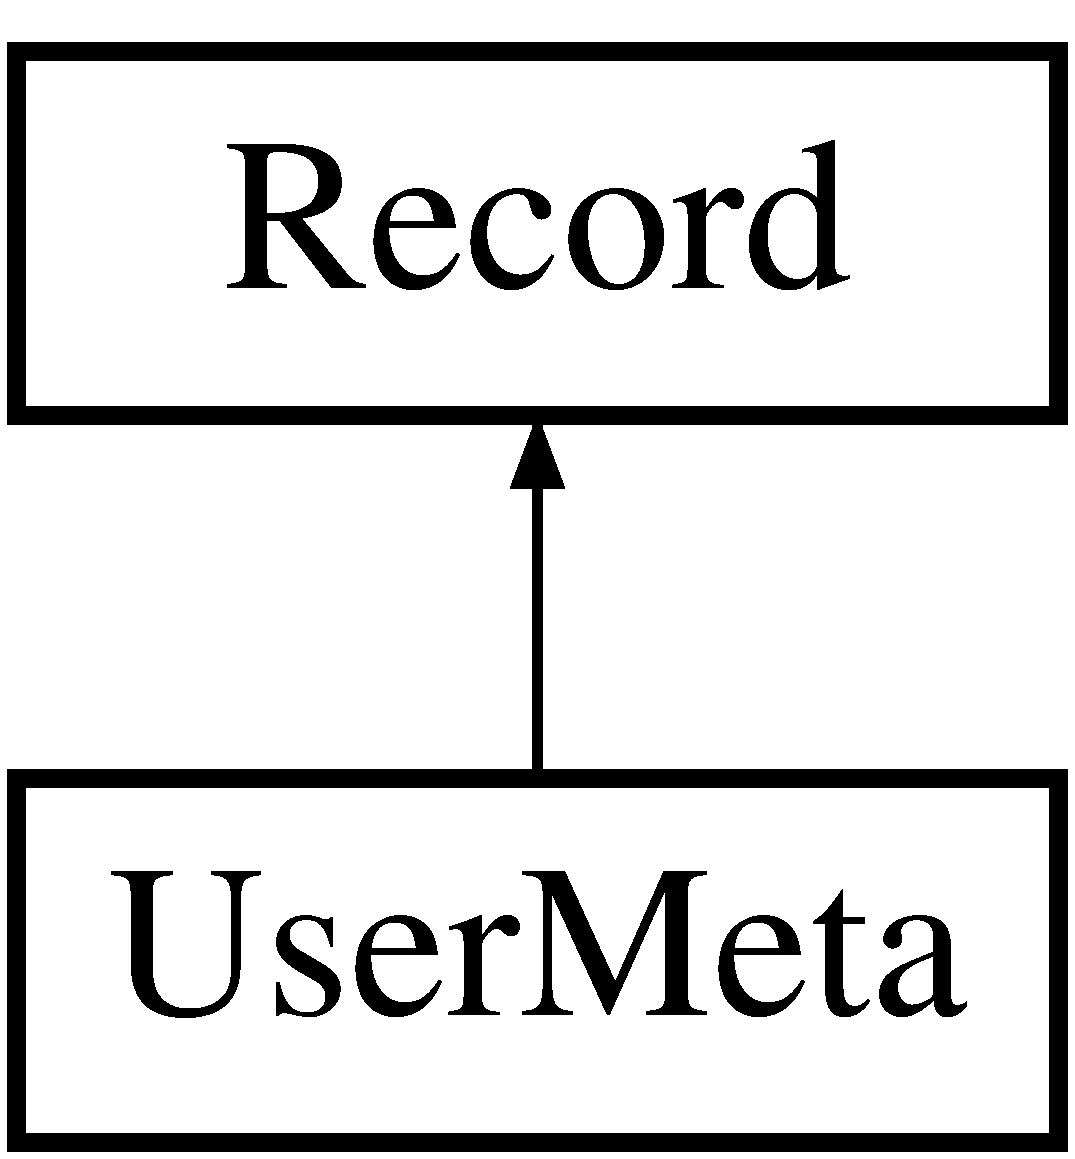
\includegraphics[height=2.000000cm]{class_user_meta}
\end{center}
\end{figure}
\subsection*{Data Fields}
\begin{DoxyCompactItemize}
\item 
\hypertarget{class_user_meta_ae8876a14058f368335baccf35af4a22b}{{\bfseries \$table} = \char`\"{}usermeta\char`\"{}}\label{class_user_meta_ae8876a14058f368335baccf35af4a22b}

\end{DoxyCompactItemize}
\subsection*{Additional Inherited Members}


The documentation for this class was generated from the following file\-:\begin{DoxyCompactItemize}
\item 
C\-:/\-Users/\-Jaime.\-Ushuaia/\-Documents/\-Git\-Hub/sleepy-\/mustache/modules/disabled/users/class.\-user.\-php\end{DoxyCompactItemize}

\addcontentsline{toc}{part}{Index}
\printindex
\end{document}
